%%%%%%%%%%%%%%%%%%%%%
% Documento maestro %
%%%%%%%%%%%%%%%%%%%%%
\documentclass{fime}

%%%%%%%%%%%%%%%%%%%%%%%%%%%%%%%%%%%%%%%%%%%
% Cargando paquetes y definiendo opciones %
%%%%%%%%%%%%%%%%%%%%%%%%%%%%%%%%%%%%%%%%%%%
% Aquí puedes cargar los paquetes que vas a usar. La clase
% fime ya incluye babel, inputenc, graphicx y los de la AMS.
% Cargar un paquete está a tu libertad (y responsabilidad).
\usepackage{hyperref}
    \hypersetup{breaklinks=true,colorlinks=true,
        linkcolor=black,citecolor=black,urlcolor=blue}
%\usepackage{titlesec}
\usepackage{float}
\usepackage{subfigure}
\usepackage{dsfont}
\usepackage{amssymb, amsmath, amsbsy} 
\usepackage{adjustbox}

\usepackage{amsmath,amsfonts,amssymb,amsthm,epsfig,epstopdf,titling,url,array}
\theoremstyle{plain}
\newtheorem{thm}{Theorem}[chapter] % reset theorem numbering for each chapter
\theoremstyle{definition}
\newtheorem{defn}[thm]{\textit{Definición}}


\setlength{\parindent}{0pt}
\setlength{\parskip}{6mm}

\usepackage{siunitx}
\usepackage{array}
\usepackage{verbatim}




%%%%%%%%%%%%%%%%%%%%%
% Definiendo campos %
%%%%%%%%%%%%%%%%%%%%%
\def\titulo{Modelos estadístico-espaciales de contaminantes del aire en el Área Metropolitana de Monterrey}
\def\autor{Jorge Armando Serna Mendoza}
\def\matricula{1985281}
\def\grado{Maestría en Ciencias de la Ingeniería }
% En caso de que el grado tenga orientación o especialidad llenar el siguiente
% campo dejando un ESPACIO INICIAL, en caso contrario, dejar vacío
\def\orientacion{con Orientación en Sistemas}
\def\fecha{Noviembre 2020} % Coloca el mes con mayúscula inicial

\def\asesor{Dr. José Arturo Berrones Santos}
\def\revisorA{Dra. Satu Elisa Schaeffer}
\def\revisorB{Dra. Bibiana Obregón Quintana}
% En el caso de que tu tesis sea de doctorado activa la variable cambiándola a \doctoradotrue
% y define tus otros dos revisores
\newif\ifdoctorado\doctoradofalse
\def\revisorC{Nombre del revisor C}
\def\revisorD{Nombre del revisor D}
% El visto bueno siempre va
\def\vobo{Dr. Simón Martínez Martínez}

%%%%%%%%%%%%%%%%%%%%%%%
% Inicia el documento %
%%%%%%%%%%%%%%%%%%%%%%%
\begin{document}

\frontmatter
\pagestyle{main}

%%% Incluye PortillasM si tu tesis es de Maestría
%%% y PortillasD si es de doctorado.
%%%%%%%%%%%%%%%%%%%%%%%%
% Primer portada: UANL %
%%%%%%%%%%%%%%%%%%%%%%%%
\thispagestyle{empty}

\begin{scshape}
\begin{center}
	{\Large \uanl} \\[5mm]
	{\large \fime} \\[5mm]
	{\large \depg}
	\vskip15mm
	\includegraphics[height=55mm]{uanl}
	\vskip12mm
	\begin{tabular}{p{11cm}}
		\centering
		{\large \titulo}
	\end{tabular}
	\vskip7mm
	{por}\\[7mm]
	{\large \autor}\\[7mm]
        % Si en tu posgrado la tesis no es opcional (como sí lo es en licenciatura), no modifiques esta línea:
	{como requisito parcial para obtener el grado de}\\[3mm]
	\MakeUppercase{\grado}\\
	\orientacion
	\vfill
	\fecha
\end{center}
\end{scshape}

%%%%%%%%%%%%%%%%%%%%%%%%%
% Segunda portada: FIME %
%%%%%%%%%%%%%%%%%%%%%%%%%
\newpage
\thispagestyle{empty}

\begin{scshape}
\begin{center}
	{\Large\uanl} \\[5mm]
	{\large\fime} \\[5mm]
	{\large\depg}
	\vskip16mm
	\includegraphics[height=50mm]{fime}
	\vskip16mm
	\begin{tabular}{p{11cm}}
		\centering
		{\large \titulo}
	\end{tabular}
	\vskip7mm
	{por}\\[7mm]
	{\large \autor}\\[7mm]
        % Si en tu posgrado la tesis no es opcional (como sí lo es en licenciatura), no modifiques esta línea:
	{como requisito parcial para obtener el grado de}\\[3mm]
	\MakeUppercase{\grado}\\
	\orientacion
	\vfill
	\fecha
\end{center}
\end{scshape}

%%%%%%%%%%%%%%%%%%%%%%%%%%%%%
% Carta del comité de tesis %
%%%%%%%%%%%%%%%%%%%%%%%%%%%%%
\newpage
\thispagestyle{empty}
\enlargethispage{5mm}

{\renewcommand{\baselinestretch}{1.1}\selectfont
\begin{center}\vspace*{-25mm}\hspace*{-10mm}
\begin{minipage}{170.5mm}
\hspace{-1.5mm}\includegraphics[height=20mm]{uanl}\hfill\raise1mm\hbox{\includegraphics[height=18.5mm]{fime}}
\hrule\vspace{0.5mm}
\scalebox{.5}{\MakeUppercase{\uanl}}\hfill\scalebox{.5}{\MakeUppercase{\fime}}\medskip
\end{minipage}
\vskip4mm{\sc\large\uanl\\\fime\\[3pt]\depg}\vskip6mm
\end{center}

Los miembros del Comité de Tesis recomendamos que la Tesis <<\titulo>>, realizada por el alumno \autor, con número de matrícula \matricula, sea aceptada para su defensa como requisito parcial para obtener el grado de \grado\orientacion.
\ifdoctorado\vskip10mm\else\vskip8mm\fi

\begin{center}
El Comité de Tesis\\
\ifdoctorado\vskip15mm\else\vskip25mm\fi

\ifdoctorado{%%%
\begin{tabular}{p{37mm}p{21mm}p{12mm}p{21mm}p{37mm}}
	\cline{2-4}
	& \multicolumn{3}{c}{\asesor} & \\
	& \multicolumn{3}{c}{Asesor}  & \\[15mm]
	\cline{1-2} \cline{4-5}
	\multicolumn{2}{c}{\revisorA} & & \multicolumn{2}{c}{\revisorB} \\
	\multicolumn{2}{c}{Revisora}   & & \multicolumn{2}{c}{Revisora}   \\[17mm]
	\cline{1-2} \cline{4-5}
	\multicolumn{2}{c}{\revisorC} & & \multicolumn{2}{c}{\revisorD} \\
	\multicolumn{2}{c}{Revisor}   & & \multicolumn{2}{c}{Revisor}   \\[2mm]
	& \multicolumn{3}{c}{Vo. Bo.} & \\[14mm]
	\cline{2-4}
	& \multicolumn{3}{c}{\vobo}   & \\
	& \multicolumn{3}{c}{Subdirector de Estudios de Posgrado}   & \\ &&&&
\end{tabular}
}\else{%%%
\begin{tabular}{p{37mm}p{21mm}p{12mm}p{21mm}p{37mm}}
	\cline{2-4}
	& \multicolumn{3}{c}{\asesor} & \\
	& \multicolumn{3}{c}{Asesor}  & \\[19mm]
	\cline{1-2} \cline{4-5}
	\multicolumn{2}{c}{\revisorA} & & \multicolumn{2}{c}{\revisorB} \\
	\multicolumn{2}{c}{Revisora}   & & \multicolumn{2}{c}{Revisora}   \\[2mm]
	& \multicolumn{3}{c}{Vo. Bo.} & \\[17mm]
	\cline{2-4}
	& \multicolumn{3}{c}{\vobo}   & \\
	& \multicolumn{3}{c}{Subdirector de Estudios de Posgrado}   & \\ &&&&
\end{tabular}
}\fi%%%

\vfill

\snnl, \MakeLowercase{\fecha}

\end{center}}

% Dedicatoria

\thispagestyle{empty}
\vspace*{17mm}

\begin{flushright}
\begin{itshape}

A mis padres, hermanas, novia y \\
a esa persona que esta en el cielo, \\
mandandome salud porque eso es lo primero.\bigskip\bigskip



\end{itshape}
\end{flushright}



\tableofcontents
\listoffigures
\listoftables

%Agradecimientos

\chapter{Agradecimientos}
\markboth{Agradecimientos}{}

Deseo agradecer a la Universidad Autónoma de Nuevo León (UANL) la oportunidad que me ha brindado de realizar mis estudios de posgrado. A la Facultad de Ingeniería Mecánica y Eléctrica (FIME) por formar parte de su alumnado. Al Consejo Nacional de Ciencia y Tecnología (CONACYT) por el apoyo económico otorgado mediante una beca de estudios de tiempo completo.

Agradezco al Posgrado en Ingeniería de Sistemas (PISIS) por ofrecerme la oportunidad de realizar mis estudios de maestría, en especial a mi asesor Arturo Berrones, quien me orientó y apoyó completamente en este proceso, y a mi revisora Elisa Schaeffer, quien me compartió sus conocimientos y por formar parte del comité de este trabajo de tesis. También, a mi revisora Bibiana Obregón, quien me ha ayudado a construir mi camino del saber y por formar parte del comité de este trabajo de tesis.

Agradezco los conocimientos brindados por mis profesores del posgrado, los comentarios y aportaciones de mis compañeros de generación y de otras generaciones, y también, agradezco las tazas de café y desvelos que compartí con mis amigos.



\mainmatter
\pagestyle{fime}

%%% Haz un documento para cada capítulo
\chapter{Resumen}
%\addcontentsline{toc}{chapter}{Resumen}
%\titleformat{\section}{\normalfont\Large\bfseries}{}{0pt}{}

\markboth{Resumen}{}

{\setlength{\leftskip}{10mm}
\setlength{\parindent}{-10mm}

\autor.

Candidato para obtener el grado de \grado\orientacion.

\uanl.

\fime.

Título del estudio: \textsc{\titulo}.

Número de páginas: 214.
%\noindent Número de páginas: 214.

%%% Comienza a llenar aquí
\paragraph{Objetivos y método de estudio:}
Encontrar entre los métodos existentes de interpolación espacial, el método que mejor pronostique niveles de contaminación del aire en el Área Metropolitana de Monterrey. Los métodos seleccionados son: Teselaciones de Voronoi, Distancia Inversa Ponderada, Funciones de Base Radial y Kriging, los cuales se utilizan para pronosticar las variables Ozono, Monóxido de Carbono, Óxido Nítrico, Bióxido de Nitrógeno, Óxidos de Nitrógeno, Partículas menores a 10 micras, Partículas menores a 2.5 micras y Bióxido de Azufre. Dichos datos de las variables son proporcionados por el Sistema Integral de Monitoreo Ambiental de la Secretaría de Desarrollo Sustentable del Gobierno de Nuevo León.

\paragraph{Contribuciones y conlusiones:}
Generar mapas que describan la calidad del aire sobre toda la área de estudio para cada contaminante, ya que cada variable sigue una distribución de los datos diferente a la del resto y así evaluar el Índice de {\sc AIRE} y {\sc SALUD} propuesto en la Norma Oficial Mexicana NOM-020-SSA1-2014, el cual indica los riesgos asociados a los niveles de contaminación de cada contaminante del aire.

\bigskip\noindent\begin{tabular}{lc}
\vspace*{-2mm}\hspace*{-2mm}Firma del asesor: & \\
\cline{2-2} & \hspace*{1em}\asesor\hspace*{1em}
\end{tabular}



\setlength{\parindent}{0pt}
\setlength{\parskip}{6mm}


\chapter{Introducción}

En este capítulo se presenta la introducción de este trabajo de tesis, donde se menciona el panorama general del problema de contaminación del aire en la Área Metropolitana de Monterrey (AMM) y cómo esta mala calidad del aire influye en la calidad de vida de sus residentes. Luego, continúa con la definición del problema, donde se delimita el área de estudio de este trabajo; seguido del objetivo, las hipótesis, alcance, motivación y justificación del presente trabajo.

\section{Panorama General}

Las ciudades o zonas metropolitanas son por naturaleza agrupamientos de personas y actividades, que por lo general son los lugares del planeta que presentan los niveles más altos de contaminación \citep{fenger}. Las actividades diarias en zonas metropolitanas generan una gran cantidad de sustancias contaminantes que modifican la composición del aire, sumado a esto, la dirección del viento propicia el esparcimiento e interacción de sustancias entre distintos lugares, es decir, las sustancias presentes en un determinado lugar pueden haber sido generadas ahí o pudieron  haber llegado de algún de otro lugar \citep{mayer}.

La presencia de dichas sustancias contaminantes provoca el deterioro de la calidad del aire, el cual propicia efectos dañinos en el medio ambiente y en la salud humana. Actualmente (octubre de 2020) el Área Metropolitana de Monterrey (AMM) presenta problemas de calidad del aire, debido al aumento de las actividades dentro de ésta, como son los centros de trabajo, centros de estudio, centros comerciales, entre otros.

El AMM cuenta con trece estaciones fijas de monitoreo bajo el encargo del Sistema Integral de Monitoreo Ambiental de la Secretaría de Desarrollo Sustentable del Gobierno de Nuevo León (SIMA), las cuales algunas de ellas han estado en funcionamiento desde el año 1993.  Los datos registrados por las estaciones de monitoreo dan una indicación de las tendencias en la calidad del aire en el AMM, sin embargo, las estaciones de monitoreo están ubicadas en sitios fijos, por lo que la información reportada solo representa microambientes alrededor de ellas.

Los estudios de evaluación de la calidad del aire tienen altos costos de muestreo o análisis, ya que se requiere de equipos de alta tecnología. Además, el representar el comportamiento de la calidad del aire con pocos puntos es un problema retante y los datos resultan ser falsos cuando se extrapolan sobre toda la región,  especialmente en las zonas metropolitanas de países en desarrollo \citep{bayraktar}.

En este trabajo, las mediciones de los contaminantes del aire de las trece estaciones de monitoreo se consideran para la determinación de puntos espaciales críticos sobre el AMM, a través de métodos de interpolación espacial deterministas y probabilísticos, para predecir valores desconocidos en  puntos no muestreados en el AMM, a partir de los valores conocidos de los puntos muestreados en las trece estaciones de monitoreo.

Diferentes métodos pueden producir resultados de puntos interpolados  distintos \citep{tang}, por lo que se requiere una comprensión completa del problema para encontrar métodos de interpolación adecuados para la región del AMM.


\subsection{Definición del Problema}

En el área de gobernación, la obligación de informar a la población sobre la calidad del aire donde residen sus habitantes es importante para establecer medidas preventivas que cuiden la salud de los habitantes. Adémas, la necesidad de conocer las mediciones históricas en una ciudad son importantes para verificar y actualizar la efectividad de los programas implementados para el control o reducción de la contaminación urbana. Sumado a esto, en el área científica los datos de mediciones de aire son componentes primordiales para entender, modelar, simular, interpolar, pronosticar y desarrollar modelos que encaminen a la creación de programas para el control de la contaminación atmosférica \citep{sima}.

Resultados de estudios científicos internacionales de la salud pública han propiciado a la creación de las Normas Oficiales Mexicanas (NOM), las cuales definen las concentraciones y los tiempos de exposición en los que un ciudadano pueda desenvolverse sin que su salud se vea afectada \citep{sima}. Dichas normas han sido aplicadas en el AMM y los resultados han mostrado que, desde el año 1993, la calidad del aire en el AMM ha inclumpido con las normas de calidad del aire establecidas por la NOM, es decir, año tras año se han registrado días que presentan mediciones de contaminantes mayores a las permitidas.

Es así que este trabajo contribuye con la selección de un modelo de interpolación espacial que mejor describa el compartamiento de contaminantes en el AMM. Dichos modelos utilizados en este trabajo, calculan valores de contaminantes en lugares dentro del AMM, donde se desconocen los niveles de contaminación, haciendo uso únicamente de los valores observados en las trece estaciones, luego este trabajo continúa con la creación de mapas que describen el comportamiento de los contaminantes del aire en el AMM, con la premisa de encontrar un modelo que describa lo mejor posible el sistema del aire en el AMM, ya que el organismo encargado de las mediciones de la calidad del aire en el AMM solo cuenta con trece estaciones de monitoreo.
 
 
\subsection{Objetivo}

El objetivo principal de este trabajo es encontrar un modelo de interpolación espacial que mejor represente los niveles de contaminación del aire en el AMM, para así continuar con la generación de mapas que describan los niveles de contaminación en la ciudad. Además, este trabajo tiene como objetivos secundarios encontrar factores que contribuyan a los niveles altos de contaminación del aire en el AMM, así como la determinación de puntos espaciales críticos dentro de la ciudad donde es importante establecer una nueva estación de monitoreo.



\subsection{Hipótesis}

Es posible estimar niveles de contaminación del aire en puntos geográficos no muestreados dentro del AMM con un nivel de error tolerable, a partir de implementar metódos de interpolación geoespaciales y deteministas, utilizando los datos de las estaciones de monitoreo del SIMA.

\subsection{Alcance}

Este trabajo utiliza datos reportados de trece estaciones fijas de monitoreo en el AMM, bajo el cargo del SIMA de la Secretaría de Desarrollo Sustentable del Gobierno de Nuevo León. Algunas estaciones de monitoreo reportan datos desde el año 1993 y actualmente se mantienen operando, aunque algunas se encuentren en estado de mantenimiento.


\subsection{Motivación}

En la Constitución Política de los Estados Unidos Mexicanos se encuentran estipulados el derecho humano a la salud y al medio ambiente saludable, es por esto que es de vital importancia que la normatividad mexicana evolucione para hacer respetar estos derechos. Si bien, el Principio de Progresividad consiste en la obligación del Estado de generar, en cada momento de la historia, una mayor y mejor protección de los derechos humanos, es así que siempre deberá de estar en constante evolución y bajo ninguna justificación en retroceso. Es por esto que se establece una obligación por parte del Estado de monitorear la calidad del aire y de comunicar los resultados a la población \citep{gpm}.

En México el uso de índices de calidad del aire como método de comunicación de riesgo ha evolucionando de manera diferente entre entidades del país, ya que mientras existen entidades como la Ciudad de México y el Estado de México, donde hay antecedentes de intervención que van más allá de los años ochentas y que, actualmente cuentan con una normatividad local al respecto; hay otras entidades como Nuevo León, Baja California, Chiapas, Chihuahua, Coahuila, Durango, Nayarit, Veracruz, Jalisco, Hidalgo, Guanajuato, Querétaro y Oaxaca; donde se han hecho esfuerzos más recientes para desarrollar sus propios índices, pero que carecen de un documento oficial en el que se defina el significado del mismo y los lineamientos para su generación, uso y difusión.

Recientemente, se han encendido alarmas ambientales decretadas en Monterrey, Nuevo León, sobre la mala calidad del aire, que posiciona a la ciudad como una de las más contaminadas del país, en lo que se refiere a material particulado, como el PM$_{10}$ y el PM$_{2.5}$ \citep{gpm}.

En el año 2018, doscientos cuatro días del año superaron los límites máximos de contaminantes en el aire establecidos en las normas ambientales \citep{oms}. En estos días, contaminantes como PM$_{2.5}$ y PM$_{10}$ ponen en riesgo la salud de la población del AMM, sobre todo si se encuentra expuesta al exterior.

La exposición al exterior durante días que superan el límite máximo de contaminación por periodos cortos o prolongados, puede producir en las personas enfermedades respiratorias y cardiovasculares, como neumonía, asma, gripe, cáncer e incluso la muerte; viéndose afectados principalmente niños y personas mayores \citep{oms}. Además el estado de Nuevo León es uno de los que reporta mayores promedios de días de hospitalización en pacientes de cero a cuatro años de edad por asma \citep{napm}.

El impulso de esta tesis está enfocado en el problema de identificar, analizar y proponer un modelo que caracterice a la red de calidad del aire en el AMM, con el fin de entender su comportamiento y evolución. Además de encontrar características importantes en ésta, para así inferir en cuales son las principales fuentes de contaminación del aire en la red.

\subsection{Justificación}

Ante la persistente mala calidad del aire que se registra en el SIMA \citep{sdsdnl}, es necesario tomar medidas preventivas contra las causas de la contaminación del aire en el AMM, por lo que se propone como metodología el uso de metodos de interpolación geoespaciales y deterministas, como herramientas para identificar, evaluar y analizar dicha problemática.

Además, la contaminación del aire en las ciudades es un grave problema ambiental, especialmente en las ciudades en desarrollo \citep{mayer}, como lo es la actual AMM.  La ruta de contaminación del aire en la atmósfera urbana consiste en la emisión y transmisión de contaminantes del aire que resultan en la contaminación del ambiente \citep{alloway}. Conocer la calidad del aire en el ambiente permite a las personas residentes del AMM saber si es propicio llevar a cabo actividades en el exterior, esto con el fin de implementar medidas preventivas en días con altas concentraciones de sustancias contaminantes que dañan la salud.

La principal razón que vuelve a este tema relevante es la poca eficiencia de métodos empleados para dar solución a la mala calidad del aire en la zona de AMM.

\section{Estructura de la Tesis}

Este trabajo de tesis está organizado como sigue:

\begin{description}
\item \textbf{Capítulo 1.} Se presenta la introducción de esta tesis, donde se describe la definición del problema, el objetivo, las hipótesis, alcances, motivación y justificación de la tesis. 
\item \textbf{Capítulo 2.} Se mencionan los antecedentes del marco teórico a seguir en este trabajo y algunas aplicaciones de los métodos usados en este trabajo.
\item \textbf{Capítulo 3.} Se describe el marco teórico de este trabajo, empezando con el análisis estadístico de los datos haciendo uso de series de tiempo, correlaciones y autocorrelaciones. Luego, de describen los conceptos y definiciones de los métodos que se implementaron en este trabajo.
\item \textbf{Capítulo 4.} Se describe la metodología implementada a partir del marco teórico antes mencionado y se expone cómo fue la experimentación de este trabajo.
 \item \textbf{Capítulo 5.} Se describen los resultados obtenidos en la experimentación y las conclusiones pertinentes a los resultados, haciendo una comparación con el estado del arte.
\end{description}







\chapter{Antecedentes y Aplicaciones}

En este capítulo se menciona el estado del arte que implementa este trabajo. Primero, se describen los resultados y técnicas que se han aplicado en el AMM para describir los niveles de contaminación del aire y se plantea la razón por la cual en este trabajo se implementan los métodos de interpolación espacial. Luego, se enuncian los antecedentes y algunas aplicaciones en orden cronológico de los métodos de interpolación utilizados en este trabajo: Teselaciones de Voronoi (TV), Funciones de Base Radial (FBR), Distancia Inversa Ponderada (DIP), Kriging Ordinario (KO) y Kriging Universal (KU).

\section{Calidad del Aire en el AMM}

El Sistema Integral de Monitoreo Ambiental (SIMA) del gobierno del estado de Nuevo León, es el organismo gubernamental encargado de reportar y dar a conocer a la población residente del AMM sobre los estándares o niveles de contaminación del aire, que se puede traducir en calidad del aire del AMM.

Actualmente, el SIMA cuenta con trece estaciones de monitoreo de calidad del aire bajo su responsabilidad, el sistema consiste en recopilar muestras de aire en los monitores y guardarlos en una base de datos. Estas estaciones de monitoreo (no todas) empezaron a trabajar desde 1993, sin embargo por cuestiones técnicas o ambientales los datos no se han podido registrar desde entonces por lo que los datos presenta ausencia de información en el periodo de tiempo 1993--2019. 

Una debilidad que presentan las redes de monitoreo (conjunto de estaciones de monitoreo) es que las mediciones tomadas por un medidor solo representa un microambiente geoespacial de contaminantes del aire, es aquí donde entra el problema de SIMA, ya que al contar con trece estaciones no es posible representar la calidad y contaminación del aire sobre toda el AMM.

Se han hecho reportes de la calidad del aire que muestran que el AMM presenta mala calidad del aire desde 1993: y a continuación se mencionan cronológicamente algunos resultados obtenidos sobre ésta. Cabe destacar que aunque se han hecho varias técnicas para describir la calidad del aire en el AMM, hasta la fecha no se ha implementado la idea de interpolar las mediciones de la muestras conocidas en las trece estaciones para tratar de describir la calidad del aire del AMM.

En 1977, se publicó en la revista \textit{Salud Pública de México} en su volúmen XIX, el artículo ``Información de la calidad en algunas ciudades del país", donde se menciona que la actividad industrial, la circulación vehicular, la erosión terrestre, el viento, la lluvia, el clima, la topografía y la actividad humana son factores responsables de la calidad del aire.

También, hace referencia a algunas propuestas para estudiar la calidad del aire por parte del gobierno, las cuales se mencionan a continuación:

\begin{itemize}
\item A fines de la década 1950 en la Dirección de Higiene Industrial de la Secretaría de Salubridad y Asistencia, se empezaron diversos estudios sobre la calidad del aire metropolitano en distintas ciudades, incluida Monterrey.
\item Más tarde en 1966, se inició un programa de estudio de la contaminación atmosférica que fue reforzado con un convenio entre la Organización Panamericana de la Salud y el Gobierno de los Estados Unidos Mexicano.
\item Hasta el día 31 de enero de 1977 se logró activar el programa en algunos estados de la República Mexicana como son: el Área metropolitana del Valle de México; Guadalajara. Jal.; Monterrey. N.L.; Ciudad Juárez. Chih.; Tijuana y Mexícali, B.C., donde fueron determinados los niveles de concentración de partículas en suspensión. En algunos sitios se investigó la precipitación pluvial,  la distribución del tamaño de las partículas, las concentraciones de bióxido de azufre y de ozono.

En resumen, el 31 de enero de 1977 estaban instaladas y en operación cuarenta y ocho unidades muestreadoras
de partículas en suspensión en grandes volúmenes de aire, distribuidas en Ia forma siguiente:

\begin{itemize}
\item 22 en el área del Valle de México.
\item 10 en Guadalajara. Jal.
\item 10 en Monterrey. N.L.
\item 2 en Ciudad Juárez. Chih.
\item 2 en Tijuana. B.C.
\item 2 en Mexicali, B.C.
\end{itemize}
\end{itemize}

En la figura \ref{red_1977}, se presenta un dibujo con las ubicaciones geográficas de diez estaciones de monitoreo del aire en el AMM.

\begin{figure}[H]
\centering
\includegraphics[width=130mm]{./red_aire_1977}
\caption{Red de monitoreo del aire localizado en Monterrey N.L.}
\label{red_1977}
\end{figure}

\begin{itemize}
\item En 2002, como parte de las publicaciones periódicas por la universidad Tecnológico de Monterrey, campus Monterrey, se publicó en la revista \textit{Calidad Ambiental, Elemento Esencial para el Desarrollo Sostenible} en su volumen VII, un análisis que resume diez años de mediciones sobre la calidad del aire del AMM, en el artículo ``Análisis de las Mediciones de la Calidad del Aire en el Área Metropolitana de Monterrey: SIMA (1993--2001)'', donde se menciona que las mediciones de la calidad del aire son componentes primordiales para entender, modelar, simular, pronosticar y desarrollar programas para el control de la contaminación atmosférica. También, alude que las mediciones son el registro histórico para verificar y actualizar la efectividad de los diversos programas implantados para la reducción o control de la contaminación urbana.

El programa SIMA del estado de Nuevo León contaba en 2002, con cinco estaciones de monitoreo en: Santa Catarina (suroeste, SO), San Bernabé (noroeste, NO), Obispado (centro, C), San Nicolás (noroeste, NE) y La Pastora (sureste, SE). Los contaminantes monitoreados en las cinco estaciones son: Monóxido de carbono (CO), partículas menores a diez micras (PM$_{10}$), ozono (O$_{3}$), óxidos de nitrógeno (NO y NO$_{2}$) y bióxido de azufre (SO$_{2}$); y los parámetros meteorológicos medidos son: dirección del viento, velocidad del viento y temperatura ambiental.

Para informar en forma clara y sencilla los niveles de contaminación existentes se utilizó el \textit{Índice Metropolitano de Calidad del Aire} (IMECA). Un valor de cien puntos IMECA se establece cuando el contaminante se encuentra en una concentración igual a la norma de calidad. Véase tabla 2.1 a tabla 2.7.
\end{itemize}

\begin{table}[H]
    \centering
    \caption{Cumplimiento a las Normas de Calidad de Aire en la AMM (1993--2000)}
	\begin{adjustbox}{max width=0.9\textwidth}
    \begin{tabular}{|c|r|r|r|r|r|c|}
\hline
         & Max/Min &\multicolumn{2}{|c|}{Norma de Calidad}  &  &\multicolumn{2}{c|}{Incumplimientos} \\ \hline
         & &ppmv &Horas &Número &Máximo ppmv &Región del máximo \\ \hline
        CO &1.17 &11.0 &8 &6 &12.9 &NE \\
        PM$_{10}$  &1.8 &150.00 (a) &24 &336 &271 (a) &SO \\
        O$_{3}$  &1.78 &0.11 &1 &152 &0.194 &NO\\
        NO$_{2}$  &1.34 &0.21 &1 &1 &0.281 &C  \\
        SO$_{2}$  &0.68 &0.13 &24 &0 &0.089 &NE\\\hline
	\multicolumn{7}{|c|}{(a) La norma y las concentraciones medidas para PM$_{10}$ están en $ug/m^{3}$.}  \\\hline
        \end{tabular}
\end{adjustbox}
    \label{cumplimiento}
\end{table}

En la tabla \ref{cumplimiento}  los contaminantes de PM$_{10}$ y Ozono, son los contaminantes que han tenido los máximos puntos IMECA. Esto es, en situaciones ambientales severas en Monterrey los IMECAs se aproximan a 200 puntos.

\begin{table}[H]
    \centering
    \caption{Días Arriba de la Norma en la AMM (1993--2000)}
	\begin{adjustbox}{max width=0.8\textwidth}
    \begin{tabular}{|c|r|r|r|c|}
        \hline
	Año &Totales * &PM$_{10}$ &Ozono &Regiones con más días \\ \hline
	1993 &80  &44  &37  &SO/NO  \\ 
	1994 &99  &84  &21  &SO/NO  \\ 
	1995 &31  &27  &4  &NO/SO  \\ 
	1996 &62  &40  &24  &NO/SO \\ 
	1997 &38  &8  &32  &SO/NO \\ 
	1998 &35  &21  &14  &SO/NO \\ 
	1999 &93  &84  &8  &NE/NO \\ 
	2000 &30  &24  &8  &SO/NO \\ 
	2001 &113  &91  &12  &SO/NO \\ \hline 
	Total &581  &423  &160  &SO/NO \\ \hline 
	Promedio &65  &47  &18  &   \\ \hline
        \end{tabular}
\end{adjustbox}
    \label{dias_arriba}
\end{table}

En la tabla \ref{dias_arriba} se reportaron el número de días que las PM$_{10}$ y Ozono han estado arriba de la norma en Monterrey desde 1993 hasta 2001. Además, indica las regiones con más días arriba de la norma, Ozono ha estado arriba de la norma dieciocho días al año en promedio, mientras que PM$_{10}$ ha rebasado la norma en cuarenta y siete días por año. En total, algunos de los contaminantes ha rebasado la norma en sesenta y cinco días por año, es decir, estos datos implican que la contaminación atmosférica en la AMM es alta 18\% de los días del año (65 días), ya sea debido a Ozono o PM$_{10}$.

\begin{table}[H]
    \centering
    \caption{Cumplimiento Anual de IMECAs Máximos en la AMM (1993--2000)}
    \begin{tabular}{|c|r|r|c|c|r|c|c|}
        \hline
	 &Promedio &\multicolumn{3}{|c|}{Máximo de IMECAs Máximos} &\multicolumn{3}{|c|}{Mínimo de IMECAs Máximos} \\ \hline
	 & &Valor &Región &Año &Valor &Región &Año \\ \hline
	CO &60 &120 &NE &1996 &30 &SE &2000 \\ 
	PM$_{10}$ &152 &255 &C &2001 &75 &SE &1997 \\ 
	O$_{3}$ &117 &192 &NO &2001 &72 &NE &1998 \\ 
	NO$_{2}$ &69 &117 &C &1993 &31 &NO &1999 \\ 
	SO$_{2}$ &32 &69 &NE &1994 &10 &C &2000 \\ \hline
        \end{tabular}
    \label{max_min}
\end{table}

\begin{table}[H]
    \centering
    \caption{Regiones con Mayores IMECAs Máximos en la AMM (1993--2000)}
    \begin{tabular}{|c|c|c|c|c|c|}
        \hline
	 Año &CO &PM$_{10}$ &Ozono &NO$_{2}$ &SO$_{2}$ \\ \hline
	 1993 &NE/C &SO/NO &SO/C &C/SO &NE/C \\
	 1994 &NE/SO &NO/SO &SO/C &C/SO &NE/C \\
	 1995 &NE/C &NO/NE &SO/NO &SO/NO &NE/C \\
	 1996 &NE/C &NO/NE &SE/SO &C/NE &NE/NO \\
	 1997 &NE/C &NO/C &SE/SO &NE/C &NE/NO \\
	 1998 &NE/SO &NO/SO &NO/SO &C/NO &NE/C \\
	 1999 &NE/SO &NE/C &SO/NO &NE/SO &NE/NO \\
	 2000 &NE/SO &SO/NO &NO/SO &NE/SO &NE/NO \\
	 2001 &NE/C &C/SE &NO/SO &NE/SO &NE/NO \\ \hline
        \end{tabular}
    \label{mayores_max}
\end{table}

La tabla \ref{max_min} muestra los máximos y mínimos que ocurrieron de 1993 a 2001 reportando la región y el año de ocurrencia del evento. La tabla \ref{mayores_max} muestra las dos regiones con mayores IMECAs máximos por año y para cada contaminante.

\begin{table}[H]
    \centering
    \caption{Cumplimiento Mensual de la Calidad del Aire en la AMM (1993--2000)}
    \begin{tabular}{|c|r|r|c|c|r|c|c|}
        \hline
	 &Relación &\multicolumn{3}{|c|}{Máximo de Promedios} &\multicolumn{3}{|c|}{Mínimo de Promedios} \\ \hline
	  &Max/Min &ppmv &Mes &Regiones &ppmv &Mes &Regiones \\ \hline
	CO &3.6 &1.800 &Enero &C/NE &0.5 &Julio &NE/NO \\ 
	PM$_{10}$ &2.6 &92 (a) &Enero &NO/SO &35 (a) &Septiembre &C/SE\\ 
	O$_{3}$ &2.7 &0.032 &Abril &SE/SO/NO &0.012 &Enero &C/NE\\ 
	NO$_{2}$ &5.4 &0.038 &Enero &C/SO &0.007 &Julio &SE/NO\\ 
	SO$_{2}$ &5.0 &0.025 &Julio &NE &0.005 &Junio &SE \\ \hline
	\multicolumn{8}{|c|}{(a) La norma y las concentraciones medidas para PM$_{10}$ están en $ug/m^{3}$.}  \\\hline
        \end{tabular}
    \label{mensual}
\end{table}

\begin{table}[H]
    \centering
    \caption{Comportamiento Hora a Hora de la Calidad del Aire en la AMM (1993--2000)}
    \begin{tabular}{|c|r|r|c|c|r|c|c|}
        \hline
	 &Relación &\multicolumn{3}{|c|}{Máximo de Promedios} &\multicolumn{3}{|c|}{Mínimo de Promedios} \\ \hline
	  &Max/Min &ppmv &Hora &Regiones &ppmv &Hora &Regiones \\ \hline
	CO  &5.0 &2.0 &7 -- 9 &C/NE &0.4 &15 -- 17 &NO/SE\\ 
	PM$_{10}$ &5.4 &150 (a) &9 -- 10 &NO/SO &28 (a) &17 -- 18 &SE/C\\ 
	O$_{3}$ &5.4 &0.054 &12 -- 13 &NE/SO &0.010 &5 -- 7 &C/SO\\ 
	NO$_{2}$ &5.2 &0.042 &8 -- 10 &C/SE &0.008 &15 -- 16 &SE/NO\\ 
	SO$_{2}$ &9.3 &0.028 &11 -- 13 &NE &0.003 &6 -- 16 &SE \\ \hline
	\multicolumn{8}{|c|}{(a) La norma y las concentraciones medidas para PM$_{10}$ están en $ug/m^{3}$.}  \\\hline
        \end{tabular}
    \label{hora}
\end{table}

La tabla \ref{mensual} muestra los máximos y mínimos de los promedios mensuales de cada contaminante de 1993 a 2000, señalando el mes y región donde sucedió el máximo y mínimo. En la tabla \ref{hora}  se muestran las concentraciones promedio hora a hora del periodo que se monitorearon los contaminantes primarios tiene un comportamiento basado en los niveles a tiempo real de: emisiones de aire, condiciones meteorológicas y reactividad química del contaminante para el AMM.

En resumen de las tablas anteriores se puede concluir que:
\setlength{\parskip}{-1cm}
\begin{enumerate}
\item Tabla \ref{cumplimiento}: Todos los contaminantes han rebasado la norma excepto el bióxido de azufre; los contaminantes con los máximos más elevados son las PM$_{10}$ y Ozono, los máximos de Ozono y PM$_{10}$ han llegado hasta 80\% arriba de la norma, y solamente la región SE ha cumplido con las normas.
\item Tabla \ref{dias_arriba}: La contaminación atmosférica en Monterrey está arriba de la norma de calidad del aire en un 18\% de los días del año debida a Ozono o PM$_{10}$. En promedio la norma de Ozono ha sido rebasada la norma diecinueve días por año y las partículas cuarenta y siete días por año.
\item Tablas \ref{max_min} y \ref{mayores_max}: En promedio el Ozono es alrededor de 120 puntos y para PM$_{10}$ es 150. También, altos niveles de Ozono se favorecen en las estaciones SO y NO. Altos niveles de PM$_{10}$ suceden en las estaciones NO y SO. Altos niveles de CO y SO$_{2}$ suceden el las estaciones NO y C. El Ozono y las PM$_{10}$ se han incrementado fuertemente en el 2001.
\item Tabla \ref{mensual}: Las altas concentraciones de Monóxido de carbono, PM$_{10}$ y Bióxido de nitrógeno sucede en diciembre--enero y las bajas en julio--agosto. Mientras que el Ozono presenta altas concentraciones en abril--mayo y sus bajas en diciembre--enero.
\item Tabla \ref{hora}: Las altas concentraciones de Monóxido de carbono, PM$_{10}$ y Bióxido de nitrógeno, suceden al iniciar la mañana y después del atardecer, y las bajas concentraciones en las últimas horas antes de anochecer. Mientras tanto, el Ozono tiene sus altas concentraciones al iniciar la tarde y sus bajas concentraciones desde el atardecer y durante la noche. En promedio, la contaminación atmosférica en la AMM es al menos cinco veces mayor al iniciar la mañana con respecto al atardecer.
\end{enumerate}
\setlength{\parskip}{6mm}

En 2017, el Proyecto de Norma Oficial Mexicana PROY-NOM-172-SEMARNAT-2017, donde se establecen los lineamientos para la obtención y comunicación del {\em Índice de Calidad del Aire y Riesgos a la Salud}, fue aprobado por el Comité Consultivo Nacional de Normalización de Medio Ambiente y Recursos Naturales. Dos años más tarde, después de haberse cumplido el procedimiento establecido en la Ley Federal sobre Meteorología y Normalización para la elaboración de normas oficiales mexicanas, el Comité Consultivo Nacional de Normalización de Medio Ambiente y Recursos Naturales aprobó la Norma Oficial Mexicana NOM-172-SEMARNAT-2019, derivada del proyecto PROY-NOM-172-SEMARNAT-2017 el 10 de octubre de 2019.

Con la implementación de los lineamientos de la Norma Oficial Mexicana NOM-172-SEMARNAT-2019 para la obtención y comunicación del {\em Índice de Calidad del Aire y Riesgos a la Salud}, se establece un método único de cálculo y los lineamientos de difusión que deberán aplicar los gobiernos estatales responsables del monitoreo de la calidad del aire, ya que la importancia del {\em Índice de Calidad del Aire y Riesgos a la Salud} no sólo consiste en informar a la población sobre el estado de la calidad del aire (buena, aceptable, mala, muy mala y extremadamente mala), sino también sobre el nivel de riesgo asociado (probables daños a la salud, dependiendo si el riesgo es bajo, moderado, alto, muy alto o extremadamente alto) y las recomendaciones de las acciones a adoptar (medidas para reducir la exposición), es decir, se busca que la información que reciba la población no solamente se refiera a la calidad del aire, sino que le permita actuar con oportunidad para proteger su salud.


Actualmente, SIMA cuenta con trece estaciones de monitoreo, de las cuales se puede observar su ubicación geográfica en la figura \ref{mapa}. Además en la tabla \ref{resumen} se muestran las características de la red de monitoreo de calidad del aire por estación, se puede ver su ubicación geográfica en coordenadas, su elevación con respecto al nivel del mar, el municipio en el que se encuentra y la fecha desde cuando entró en operación cada estación.


\begin{table}[H]
\centering
\caption{Características de las estaciones de monitoreo del SIMA}
\begin{adjustbox}{max width=0.9\textwidth}
\small{\begin{tabular}{lllllll}
No. & Municipio                                                                        & Zona       & Simbología & \begin{tabular}[c]{@{}l@{}}Coordenadas\\ Geográficas\end{tabular}                                           & Elevación & Operando desde \\  \hline
1   & \begin{tabular}[c]{@{}l@{}}Guadalupe,\\ Nuevo León\end{tabular}                  & Sureste    & SE         & \begin{tabular}[c]{@{}l@{}}25.668 N, 100.249 W\end{tabular}     & 492 msnm  & 20/Nov/1992    \\ \hline
2   & \begin{tabular}[c]{@{}l@{}}San Nicolás\\ de los Garza,\\ Nuevo León\end{tabular} & Noreste    & NE         & \begin{tabular}[c]{@{}l@{}}25.75 N, 100.255 W\end{tabular}      & 476 msnm  & 20/Nov/1992    \\ \hline
3   & \begin{tabular}[c]{@{}l@{}}Monterrey,\\ Nuevo León.\\ Obispado\end{tabular}      & Centro     & CE         & \begin{tabular}[c]{@{}l@{}}25.67 N, 100.338 W\end{tabular}      & 560 msnm  & 20/Nov/1992    \\ \hline
4   & \begin{tabular}[c]{@{}l@{}}Monterrey,\\ Nuevo León.\\ Sn. Bernabé\end{tabular}   & Noroeste   & NO         & \begin{tabular}[c]{@{}l@{}}25.757 N, 100.366 W\end{tabular}     & 571 msnm  & 20/Nov/1992    \\ \hline
5   & \begin{tabular}[c]{@{}l@{}}Santa\\ Catarina,\\ Nuevo León\end{tabular}           & Suroeste   & SO         & \begin{tabular}[c]{@{}l@{}}25.676 N, 100.464 W\end{tabular}     & 694 msnm  & 20/Nov/1992    \\ \hline
6   & \begin{tabular}[c]{@{}l@{}}García,\\ Nuevo León\end{tabular}                     & Noroeste 2 & NO2        & \begin{tabular}[c]{@{}l@{}}25.783 N, 100.586 W\end{tabular}    & 716 msnm  & 24/Jul/2009    \\ \hline
7   & \begin{tabular}[c]{@{}l@{}}Escobedo,\\ Nuevo León\end{tabular}                   & Norte      & N          & \begin{tabular}[c]{@{}l@{}}25.800 N, 100.344 W\end{tabular}    & 528 msnm  & 22/Dic/2009    \\ \hline
8   & \begin{tabular}[c]{@{}l@{}}Apodaca,\\ Nuevo León\end{tabular}                    & Noreste 2  & NE2        & \begin{tabular}[c]{@{}l@{}}25.777 N, 100.188 W\end{tabular}    & 432 msnm  & 01/Jun/2011    \\ \hline
9   & \begin{tabular}[c]{@{}l@{}}Juárez,\\ Nuevo León\end{tabular}                     & Sureste 2  & SE2        & \begin{tabular}[c]{@{}l@{}}25.646 N, 100.096 W\end{tabular}   & 387 msnm  & 01/Oct/2012    \\ \hline
10  & \begin{tabular}[c]{@{}l@{}}San Pedro\\ Garza\\ García,\\ Nuevo León\end{tabular} & Suroeste 2 & SO2        & \begin{tabular}[c]{@{}l@{}}25.665 N, 100.413 W\end{tabular}   & 636 msnm  & 06/Feb/2014    \\ \hline
11  & \begin{tabular}[c]{@{}l@{}}Cadereyta\\ de Jiménez,\\ Nuevo León\end{tabular}     & Sureste 3  & SE3        & \begin{tabular}[c]{@{}l@{}}25.36 N, 99.9955 W\end{tabular} & 340 msnm  & 21/Ago/2017    \\ \hline
12  & \begin{tabular}[c]{@{}l@{}}UANL, San\\ Nicolás,\\ Nuevo León\end{tabular}        & Norte 2    & N2         & \begin{tabular}[c]{@{}l@{}}25.5749 N, 100.2489 W\end{tabular} & 630 msnm  & 04/Oct/2017    \\ \hline
13  & \begin{tabular}[c]{@{}l@{}}Monterrey,\\ Nuevo León\end{tabular}                  & Sur        & S          & \begin{tabular}[c]{@{}l@{}}25.7295 N, 100.3099 W\end{tabular} & 520 msnm  & 04/Oct/2017   
\end{tabular} }
\end{adjustbox}
\label{resumen}
\end{table}

\begin{figure}[H]
\centering
\includegraphics[width=130mm]{./mapa}
\caption{Mapa del AMM con las trece estaciones meteorológicas marcadas por un símbolo de posición geográfica \citep{mapa}}
\label{mapa}
\end{figure}


\begin{table}[H]
\centering
\caption{Variables y contaminantes medidos por SIMA}
\begin{adjustbox}{max width=0.9\textwidth}
\begin{tabular}{|c|c|c|c|}
\hline
Nombre del contaminante &Nomenclatura SIMA &Nomenclatura MEEAMM &Unidad de medición \\ \hline
Particulas menores a 10 micras &PM$_{10}$ &PM$_{10}$ &Ugr /m$^{3}$\\
Particulas menores a 2.5 micras &PM$_{2.5}$  &PM$_{2.5}$ &Ugr /m$^{3}$\\
Ozono &O$_{3}$ &O$_{3}$ &ppb\\   
Óxido Nítrico &NO &NO &ppb\\ 
Bióxido de Nitrógeno &NO$_{2}$ &NO$_{2}$ &ppb\\
Oxídos de Nitrógeno &NO$_{X}$ &NO$_{X}$ &ppb\\
Bióxido de Azufre &SO$_{2}$ &SO$_{2}$ &ppb\\
Monóxido de Carbono &CO  &CO &ppb\\
Temperatura ambiental &TOUT &Temperature &$^{\circ}$C\\
Precipitación pluvial &RAINF &Rainfall &mn/h\\
Humedad relativa &HR &Humidity &\% \\
Presión barométrica &PRES &Pressure &mnHg \\
Radiación solar &SR & Solar &kWh/m$^{2}$ \\
Velocidad del ciento &WSR &Velocity &Km/h \\
Dirección del viento &WDR &Direction &Grado azimutal\\ \hline
\multicolumn{4}{|c|}{Abreviación del título de esta tesis Modelos Estadístico Espacial de contaminantes del aire en el AMM (MEEAMM) } \\ \hline
\end{tabular}
\end{adjustbox}
\label{variables}
\end{table}

En las trece estaciones con las que cuenta el SIMA, se miden y registran quince variables, las cuales se muestran en la figura \ref{variables}; en la cual se muestra el nombre de la variable, la nomenclatura asignada por SIMA, la nomenclatura asignada para este trabajo de tesis y que se emplea en el código fuente \citep{sernagit} (MEAMM, pos sus siglas de Modelo Espacial de contaminantes del Área metropolitana de Monterrey) y la unidad en la que se mide cada variable.

Partiendo de las concentraciones base indicadas en la tabla \ref{base} se crea el Índice {\sc AIRE} y {\sc SALUD} con base en la Norma Oficial Mexicana  PROY-NOM-172-SEMARNAT-2017 (ver tabla \ref{base}).

\begin{table}[H]
\centering
\caption{Concentraciones base para el cálculo del { \em Índice AIRE y SALUD} para cada contaminante}
\begin{adjustbox}{max width=0.9\textwidth}
\begin{tabular}{|c|c|}
\hline
Contaminante &Concentración base\\ \hline
PM$_{10}$ &Concentración promedio móvil ponderado de 12 horas \\
PM$_{2.5}$ &Concentración promedio móvil de 12 horas \\
O$_{3}$ &Concentración promedio móvil de 8 horas \\
CO &Concentración promedio móvil de 8 horas \\
NO$_{2}$ &Concentración promedio horaria \\
SO$_{2}$ &Concentración promedio de 24 horas \\ \hline
\end{tabular}
\end{adjustbox}
\label{base}
\end{table}

Las bandas de calidad del aire y riesgo que componen el {\em Índice AIRE y SALUD} se construyen considerando los intervalos de concentración señalados en la Norma Oficial Mexicana PROY-NOM-172-SEMARNAT-2017, según aplique al contaminante criterio. Particularmente, los límites superiores del intervalo de la banda “Aceptable” concuerdan con los valores establecidos en las Norma Oficial Mexicana NOM-020-SSA1-2014.

\begin{table}[H]
\centering
\caption{Obtención del {\em Índice AIRE y SALUD} para PM$_{10}$}
\begin{adjustbox}{max width=0.9\textwidth}
\begin{tabular}{|c|c|c|}
\hline
Calidad del aire & Nivel de riesgo & Intervalo de PM$_{10}$ \\ \hline
Buena &Bajo &$\leq50$ \\
Aceptable &Moderado &$>50, \leq75$ \\
Mala &Alto &$>75, \leq155$ \\
Muy Mala &Muy Alto &$>155, \leq235$ \\
Extremadamente Mala &Extremadamente Alto &$>235$ \\ \hline
\end{tabular}
\end{adjustbox}
\label{basepm10}
\end{table}

\begin{table}[H]
\centering
\caption{Obtención del {\em Índice AIRE y SALUD} para PM$_{2.5}$}
\begin{adjustbox}{max width=0.9\textwidth}
\begin{tabular}{|c|c|c|}
\hline
Calidad del aire & Nivel de riesgo & Intervalo de PM$_{2.5}$ \\ \hline
Buena &Bajo &$\leq25$ \\
Aceptable &Moderado &$>25, \leq45$  \\
Mala &Alto &$>45, \leq79$ \\
Muy Mala &Muy Alto &$>79, \leq147$ \\
Extremadamente Mala &Extremadamente Alto &$>147$ \\ \hline
\end{tabular}
\end{adjustbox}
\label{basepm25}
\end{table}

\begin{table}[H]
\centering
\caption{Obtención del {\em Índice AIRE y SALUD} para O$_{3}$}
\begin{adjustbox}{max width=0.9\textwidth}
\begin{tabular}{|c|c|c|}
\hline
Calidad del aire & Nivel de riesgo & Intervalo de O$_{3}$ \\ \hline
Buena &Bajo &$\leq0.051$ \\
Aceptable &Moderado &$>0.051, \leq0.070$ \\
Mala &Alto &$>0.070, \leq0.092$ \\
Muy Mala &Muy Alto &$>0.092, \leq0.114$ \\
Extremadamente Mala &Extremadamente Alto &$>0.114$ \\ \hline
\end{tabular}
\end{adjustbox}
\label{baseo3}
\end{table}

\begin{table}[H]
\centering
\caption{Obtención del {\em Índice AIRE y SALUD} para NO$_{2}$}
\begin{adjustbox}{max width=0.9\textwidth}
\begin{tabular}{|c|c|c|}
\hline
Calidad del aire & Nivel de riesgo & Intervalo de NO$_{2}$ \\ \hline
Buena &Bajo &$\leq0.107$ \\
Aceptable &Moderado &$>0.107, \leq0.210$  \\
Mala &Alto &$>0.210, \leq0.230$ \\
Muy Mala &Muy Alto &$>0.230, \leq0.250$ \\
Extremadamente Mala &Extremadamente Alto &$>0.250$ \\ \hline
\end{tabular}
\end{adjustbox}
\label{baseno2}
\end{table}

\begin{table}[H]
\centering
\caption{Obtención del {\em Índice AIRE y SALUD} para SO$_{2}$}
\begin{adjustbox}{max width=0.9\textwidth}
\begin{tabular}{|c|c|c|}
\hline
Calidad del aire & Nivel de riesgo & Intervalo de SO$_{2}$ \\ \hline
Buena &Bajo &$\leq0.008$ \\
Aceptable &Moderado &$>0.008, \leq0.110$ \\
Mala &Alto &$>0.110, \leq0.165$ \\
Muy Mala &Muy Alto &$>0.165, \leq0.220$ \\
Extremadamente Mala &Extremadamente Alto &$>0.220$ \\ \hline
\end{tabular}
\end{adjustbox}
\label{baseso2}
\end{table}

\begin{table}[H]
\centering
\caption{Obtención del {\em Índice AIRE y SALUD} para CO}
\begin{adjustbox}{max width=0.9\textwidth}
\begin{tabular}{|c|c|c|}
\hline
Calidad del aire & Nivel de riesgo & Intervalo de CO \\ \hline
Buena &Bajo &$\leq8.75$ \\
Aceptable &Moderado &$>8.75, \leq11.00$  \\
Mala &Alto &$>11.00, \leq13.30$ \\
Muy Mala &Muy Alto &$>13.30, \leq15.50$ \\
Extremadamente Mala &Extremadamente Alto &$>15.50$ \\ \hline 
\end{tabular}
\end{adjustbox}
\label{baseco}
\end{table}


La difusión de riesgos relacionada al {\em Índice AIRE y SALUD} consistirá en el establecimiento de cinco bandas que estarán asociadas a cinco colores (verde, amarillo, naranja, rojo y morado) como se describe en la tabla \ref{categorias}. El Índice AIRE Y SALUD sólo tiene fines de información para prevenir a la población en una ciudad o localidad en una hora determinada, estos riesgos estan asociados a los niveles de contaminación de cada contaminante descritos en la tablas \ref{basepm10}, \ref{basepm25}, \ref{baseo3}, \ref{baseno2}, \ref{baseso2}, y \ref{baseco}.

\begin{table}[H]
\centering
\caption{Categorías del {\em Índice AIRE y SALUD}}
\begin{adjustbox}{max width=0.9\textwidth}
\begin{tabular}{|c|c|c|c|}
\hline
Calidad del aire & Nivel de riesgo  &Color \\ \hline
Buena &Bajo &Verde \\ \hline
Aceptable &Moderado &Amarillo \\ \hline
Mala &Alto &Naranja \\ \hline
Muy Mala &Muy Alto &Rojo \\ \hline
Extremadamente Mala & Extremadamente Alto &Morado \\ \hline
\end{tabular}
\end{adjustbox}
\label{categorias}
\end{table}








\section{Métodos de Interpolación}

Esta sección presenta brevemente los diferentes métodos de interpolación utilizados en este trabajo de tesis, como son los ya conocidos; Teselaciones de Voronoi, Funciones de Base Radial, Distancia Inversa Ponderada, Kriging Universal y Kriging Ordinario. Cabe destacar que los métodos de interpolación espacial mencionados difieren en sus supuestos, perspectiva local o global y naturaleza determinista o estocástica.

\subsection{Teselaciones de Voronoi}
Las Teselaciones de Voronoi o Diagramas de Voronoi (TV) son estructuras geométricas que aparecen con regularidad en la naturaleza, por esta razón se han redescubierto varias veces a lo largo de la historia, reciben su nombre en honor al matemático ruso Georgy Voronoi, también son conocidas como Polígonos de Thiessen (por el meteorólogo estadounidense Alfred Thiessen), Teselación de Dirichlet (por el matemático alemán Peter Gustav Lejeune Dirchlet), Celdas de Wigner-Seitz (por el físico matemático húngaro Eugene Wigner y el físico estadounidense Frederick Seitz) o Zonas de Brillouin (por el físico francés León Nicolás Brillouin \citep{aurenhammer}.

En 1664, el filósofo y matemático francés Descartes afirmó que el sistema solar se compone de \textit{vórtices}; considerados como cualquier tipo de flujo circular o rotatorio que posee vorticidad. Las ilustraciones de Descartes muestran una descomposición del espacio en regiones convexas, donde cada una de éstas está compuesta de la materia que gira alrededor de una de las estrellas fija \citep{aurenhammer}.

En 1850, Dirichlet formalizó el estudio de formas cuadráticas definidas positivas (forma especial de un Diagrama de Voronoi) en $\mathbb{R}^{2}$ y $\mathbb{R}^{3}$ \citep{dirichlet}. Cuatro años depués en 1854, el médico inglés John Snow (padre de la epidemiología moderna), hizo un análisis del brote de cólera que azotó la ciudad de Londres, mediante el uso del método geográfico \citep{doval}.

En 1908, Voronoi precisó el estudio de formas cuadráticas definidas positivas en $\mathbb{R}^{n}$. Un año más tarde en 1909, el geólogo, cristalógrafo y mineralogista ucraniano Boldyrev (Anatoly Kapitonovich) estimó las reservas de minerales en un depósito usando la información obtenida de taladros, nombrando a las regiones de Voronoi \textit{áreas de polígonos de influuencia.}

En 1911, Thiessen analizó datos meteorológicos de estaciones pluviométricas, donde a las regiones las nombró \textit{polígonos de Thiessen}. En 1927, el cristalógrafo suizo Paul Niggli desarrolló la teoría en Cristalografía \citep{manzoor}. Dos años después en 1929, el matemático ruso Boris Deloné (Delaunay) fue el primero en acuñar el término \textit{Dominio de Dirichlet} y el término \textit{Región de Voronoi.}

En 1933,  Wigner y Seitz describieron las regiones de Voronoi para los puntos dispuestos en una retícula en el espacio tridimensional \citep{okabe}. En 1949, el demógrafo estadounidense Donald Bogue, usó los polígonos de Voronoi definidos alrededor de centros metropolitanos.

En 1965, G.\ S.\ Brown estimó la intensidad de población de los árboles en un bosque, definiendo una región de Voronoi para un árbol individual, llamándola el \textit{área potencialmente disponible} (APA) de un árbol \citep{brown}. En 1985, L.\ Hoofd et al. definieron las regiones de Voronoi con respecto a los centros de los capilares en secciones de tejido \citep{turek}. Dos años después en 1987, V.\ Icke y R.\ Van de Weygaert realizaron una partición del espacio por medio de un proceso de diagramas de Voronoi \citep{icke}.



\subsection{Funciones de Base Radial}
Las Funciones de Base Radial (FBR) comprenden un gran grupo de interpoladores exactos, los cuales utilizan una \textit{ecuación básica} que depende de la distancia entre los puntos de muestreo y el punto interpolado. Dicha ecuación toma en cuenta que la función de interpolación minimiza una función que representa alguna medida de suavidad \citep{aguilar}.

Un tipo particular de las funciones de base radial son las de \textit{soporte global}, las cuales son funciones infinitamente diferenciables y con valor real no nulo en todos los puntos de su dominio, y donde algunas contienen un parámetro libre, llamado \textit{parámetro de forma}. El uso de este tipo de funciones básicas produce una matriz de interpolación que sirve para interpolar suavemente y generar zonas continuas sobre superficies discontinuas \citep{arias}.

Algunos tipos de funciones de base radial de soporte global más populares en la literatura que se usan en este trabajo son: \textit{Multicuadrática} (FBRM), \textit{Inversa multicuadrática} (FBRIM), \textit{Gaussiana} (FBRG), \textit{Biarmónica} o \textit{Lineal} (FBRL), \textit{Triarmónica} o \textit{Cúbica} (FBRC)y \textit{Thin Plate Spline} (FBRTPS). Todas ellas han tenido buena aceptación debido a que el sistema asociado de ecuaciones lineales resulta ser invertible, incluso si la distribución de los puntos no presenta regularidad \citep{arias}.

En 1977, A.\ Talmi y G.\ Gilat plantearón los antecedentes matemáticos para la construcción de funciones de base radial en su trabajo \textit{Method for Smooth Approximation of Data} \citep{talmi}. La aplicación de estos métodos de interpolación a grandes volúmenes de datos presenta una serie de problemas, como el alto costo computacional, un aumento en la inestabilidad de la solución encontrada y la influencia de todos los puntos de muestreo en cada valor interpolado \citep{lazzaro}.

En 1982, R.\ Franke recomendó que el BRFM es el que proporciona los mejores resultados en términos de evaluación estadística y visual de la superficie modelizada \citep{franke}. Ya que una ecuación de topografía basada en la suma multicuadrática aplica un concepto geométrico simple, donde la suavidad y la forma de la transición entre los puntos de datos están controladas principalmente por las características del cuadricular básico utilizado en la suma \citep{hardy}.

En 1990, R.\ L.\ Hardy comentó que el BRFM funciona bien como método de interpolación, cuando las mediciones de potencial o temperatura en la superficie de la tierra se obtienen en estaciones meteorológicas dispersas \citep{hardy1990}.

En 1992, F.\ Girosi mencionó que las funciones de base radial son un enfoque adecuado cuando la aproximación a las llamadas técnicas de aprendizaje de las redes neuronales conducen a problemas de interpolación de muy alta dimensión con datos dispersos, debido a su disponibilidad en dimensiones arbitrarias y a su suavidad \citep{girosi}.

En 1996, T.\ Sonar utilizó funciones de base radial para la reconstrucción local de soluciones dentro de algoritmos que resuelven leyes de conservación numéricamente hiperbólicas. Hasta entonces era habitual emplear una aproximación polinómica de bajo orden (en su mayoría lineal) para este propósito; pero resultó que las funciones de base radial, especialmente las FBRTPS, ayudan a mejorar la precisión de los métodos de volumen finito, sobre todo para resolver las ecuaciones hiperbólicas, debido a su capacidad para aproximarse localmente con gran precisión \citep{sonar}.

En 2002, A.\ Kremper, T.\ Schanze y R.\ Eckhorn usaron datos provenientes de una pantalla que muestra la lectura de una cámara que sirve como ojo de un robot. Las imágenes representan objetos que el robot debería reconocer, por ejemplo, un muro con el que no debería estrellarse, otro robot, un humano o cualquier otro objeto. Sin embargo, se tuvo el problema que cada uno de estos datos debía interpolarse para que el robot fuera capaz de reconocer otras situaciones similares, ya que las imágenes tenían variaciones como: ángulos, escalas, etc. Para este problema se encontró que usando interpolaciones de FBR, el robot lograba identificar una mayor cantidad de datos \citep{kremper}.




\subsection{Distancia Inversa Ponderada}

La interpolación de Distancia Inversa Ponderada (DIP) se aplica ampliamente por los científicos de la tierra \citep{ware} y en la cartografía automatizada, ya que realiza el cálculo de una superficie cuadriculada bidimensional a partir de un conjunto de puntos dispersos con valores conocidos \citep{armstrong}. En las geociencias, la idea de usar DIP se encuentra encaminada a evaluar la contaminación en un punto de referencia, a partir de las mediciones realizadas por las estaciones de monitoreo \citep{vogl}. DIP se basa en la premisa de que las predicciones son una combinación lineal de datos disponibles \citep{xie}, donde los pesos dependen de la distancia entre las estaciones de monitoreo con un exponente arbitrario y en consecuencia, son exógenos con respecto a los datos \citep{armstrong}.

En 1996, P.\ Bartier y C.\ Keller presentaron una metodología de interpolación que aborda explícitamente la variación de la superficie a través de límites poligonales temáticos. El método de interpolación de DIP se implementó para permitir a los usuarios definir el grado esperado de brusquedad de la superficie a lo largo de los límites temáticos utilizando una matriz de transición. El procedimiento se demostró utilizando como caso de estudio, una superficie interpolada de geoquímica de níquel modificada por límites estratigráficos de terreno \citep{bartier}.

En 2004, R.\ L.\ Hough realizó una evaluación de riesgo de exposición a metales en subgrupos de población que viven y cultivan alimentos en sitios urbanos, donde se utililizó la interpolación por DIP en las concentraciones de metales en las verduras, para evaluar el riesgo de exposición a las poblaciones humanas \citep{hough}.

En 2005, J.\ Currie y M.\ Neidel examinaron el impacto de la contaminación del aire en la muerte infantil en California durante la década de 1990. Aquí utilizaron DIP en niveles de contaminación de CO del aire y descubrieron que las reducciones en el monóxido de carbono durante la década de 1990 salvaron aproximadamente 1000 vidas infantiles en California \citep{currie}.

En 2009, O.\ Babak y C.\ V\ Deutsch presentaron un enfoque para integrar controles estadísticos, como la mínima varianza de error en la interpolación de DIP. Mencionando que el exponente óptimo y el número de datos pueden calcularse global o localmente, y que las medidas de incertidumbre y suavidad local pueden derivarse de estimaciones de DIP \citep{babak}.

En 2012, F.\ Chen y C.\ Liu utilizaron DIP para estimar la distribución de lluvia en Taiwán, con un total de cuarenta y seis estaciones y datos de lluvia entre 1981 y 2010, de las cuales doce estaciones pertenecientes a la Asociación de Riego de Taichung (TIA), se usaron para la validación cruzada. Encontrando que los parámetros óptimos para DIP en la interpolación de datos de lluvia tienen un radio de influencia de hasta 10--30 km en la mayoría de los casos y que, usando DIP en estos datos de interpolación pueden obtenerse resultados más precisos durante la estación seca que en la temporada de inundaciones. En conclusión, obtuvieron que los altos valores de coeficiente de correlación (más de 0.95) confirmaron a DIP como un método adecuado de interpolación espacial para predecir los datos probables de lluvia en Taiwán \citep{chen}.



\subsection{Kriging Ordinario}

El término {\em Krigeage} fue acuñado por P.\ Carlier en reconocimiento de D.G.\ Krige por su innovación pionera para estimar las concentraciones de oro y otros metales en el suelo \citep{oliver}.

El método Kriging Ordinario (KO) predice valores en sitios no visitados a partir de datos de muestra dispersos, basados en un modelo estocástico de variación espacial contínua; teniendo en cuenta conocimiento de la variación espacial representada en el \textit{variograma} o \textit{función de covarianza}. 

En 1963, G.\ Matheron en su libro \textit{Principles of geostatistics} introdujo al idioma inglés el termino \textit{Kriging} \citep{matheron1963} y dos años después, en 1965, en su tesis doctoral colocó la técnica dentro del marco de la teoría de procesos aleatorios \citep{matheron1965}. El trabajo de Matheron no estaba aislado, ya que trabajos como los de; Andréi \citet{kolmogorov1939,kolmogorov1941}, Herman \citet{wold} y \citet{wiener}, ya habían llegado cerca del kriging, pero en el tiempo más que en el espacio \citep{cressie1990}.

En 1990, M.\ Oliver y R.\ Webster comentaron que los sistemas de información geográfica pueden mejorarse agregando procedimientos para el análisis espacial geoestadístico a las estaciones de monitoreo existentes, ya que los datos distribuidos espacialmente se comportan más como variables aleatorias, donde la teoría de variables regionalizadas proporciona un conjunto de métodos estocásticos que minimizan el error de predicción \citep{oliver1984}.

En 1994, R.\ Dimitrakopoulos y X.\ Luo aludieron que se puede usar una representación general de `anisotropía zonal' para una covarianza espacio-temporal positiva. Se demostró que una covarianza espacio-temporal definida estrictamente positiva, se puede asegurar la unicidad de la solución del sistema Kriging \citep{dimitrakopoulos}. Aquí resultados de Dimitrakopoulos y Luo se basaron en el enfoque de \citet{buxton}, así como en los de \citet{bilonick2, bilonick1}.

En 2004, L.\ Bel utilizó un estimador no paramétrico y un modelo de transporte químico para producir mapas de concentración de Ozono sobre el área de París y compararlos con los mapas obtenidos con los métodos de Kriging clásicos. Bel mostró que al tener  pocas estaciones KO resulta ser malo interpolando cuando se aplíca con los estimadores clásicos \citep{bel}.

En 2007, M.\ Villatoro, C.\ Henríquez y F.\ Sancho hicieron una comparación entre KO y DIP de mediciones de materiales en el suelo. Para el KO se calcularon los semivariogramas y también se determinó que el modelo esférico fue el de mejor ajuste. Ambos métodos tuvieron un desempeño similar, el KO fue superior al predecirlo de una mejor manera \citep{villatoro}.

En 2015, O.\ Delgado y J.\ Martínez emplearon el método KO para construir el mapa de ruido de la Ciudad de Cuenca, Ecuador; su trabajo partió con la determinación de los sitios de muestreo sobre la base de la densidad de tráfico, luego se registraron las mediciones de ruido ambiente y posteriormente se sistematizó y evaluó la información levantada a través del método KO, con lo cual se elaboró el mapa de ruido de la ciudad \citep{delgado}.

Formas más elaboradas de Kriging se encuentran desarrollando para abordar problemas cada vez más complejos en la ingeniería petrolera, minería y geología, meteorología, ciencia del suelo, agricultura de precisión, contaminación, salud pública, pesca, ecología vegetal y animal, teledetección e hidrología.



\subsection{Kriging Universal}

El método Kriging Universal (KU) a diferencia del método KO supone que la media de los datos $m(x)$ tiene una dependencia funcional de la ubicación espacial y puede ser aproximada por un modelo con la ecuación \citep{kumar}:
\begin{equation}
 \mu(x) = \sum_{i=1}^{k} a_{i}f_{i}(x),
\end{equation}
donde $a_{i}$ son los coeficientes a estimar a partir de los datos, $f_{i}$ es una función básica de coordenadas espaciales y $k$ es el número de funciones utilizadas en el modelo.

En 1988,  S.\ Dingman,  D.\ Seely y R.\ Reynolds estudiaron las mediciones de los equilibrios químicos y del agua para las cuencas de drenaje y los cuerpos de agua superficiales. Mencionando que los errores en sus predicciones usando KU pueden deberse a fallas de los medidores individuales para recolectar la cantidad de precitación que realmente cae, errores del operador o fallas de la red de regado para muestrear adecuadamente la región de interés. Sus resultados mostraron que el KU a diferencia de KO presenta un error considerablemente más paqueño, por lo que es preferible como base para estimaciones puntuales \citep{dingman}.

En 2002, P.\ Kanaroglou, N.\ Soulakellis y N.\ Sifakis demostraron que el KU puede usarse para obtener estimaciones razonables para datos con valores faltantes para la evaluación de la distribución espacial de contaminantes del aire. Usaron imágenes de satélite implementando el método de Análisis de Textura Diferencial, el cual se utiliza para medir el espesor óptico del aerosol en lo visible, que se correlaciona altamente con la calidad del aire. Con este método, la presencia de nubes o cambios en la cobertura del suelo producen parches de valores perdidos, los que se recuperaron usando KU \citep{kanaroglou}.

En 2011, L.\ Mercer et al. mencionaron que el método KU es un buen método de interpolación para, valga la redundancia, interpolar mediciones de nitrógeno (NO$_{X}$) en Los Ángeles, C.A. \citep{mercer}. Dos años después en 2013, P.\ Sampson et. al. presentaron un modelo de KU para interpolar datos de partículas menores a dos punto cinco micras (PM$_{2.5}$), de estaciones de monitoreo en los EE.\ UU., reflejando un nivel muy alto de precisión de predicción bajo el método de validación cruzada \citep{sampson}.

En 2016, I.\ Ki\v{s} et al. hicieron una comparación entre los metodos KO Y KU, sus resultados arrojaron que el método KU predice mejor que KO cuando los datos presentan una tendencia espacial lineal, ya que esta técnica se desarrolló precisamente para identificar y calcular tendencias en los datos, es decir, para describir la regresión y dar mejores resultados de mapeo \citep{kivs}.  








































\chapter{Marco Teórico}


En este capítulo se exponen los conceptos que explican el comportamiento de los datos y la suma importancia de conocer las características y comportamiento para hacer uso de los datos en la experimentación de este trabajo de tesis. Primero se habla sobre las \textit{series de tiempo} y las caracterísiticas que éstas deben cumplir para poder decir que estadísticamente los datos con los que contamos son útiles para la experimentación. Luego, se exponen los conceptos de \textit{autocorrelación}, \textit{autocovarianzas} y \textit{variograma}, y cómo estos conceptos ayudan a entender el comportamiento de los datos y a mejorar los resultados de la experimentación.

\section{Análisis Estadístico}

Se utilizan herramientas estadísticas para conocer el comportamiento de los datos, primero se usan series de tiempo para graficar los datos de contaminantes por estaciones y observar las características de éstas. Luego, se verifica si las series cumplen con la propiedad de ser estacionarias en el tiempo. Después se calcular los correlaciones y autocorrelaciones de los contaminantes por estación y por último, se calcula el variograma, el cual se utiliza como parámetro para encontrar el mejor método de interpolación de los métodos geoespaciales.

\subsection{Series de Tiempo}

Una \textit{serie de tiempo} es una secuencia cronológica de observaciones sobre una variable de interés \citep{montgomery}. Por ejemplo, la figura \ref{serie} muestra el rendimiento del mercado de los valores del tesoro de EE.\ UU.\ con vencimiento constante a 10 años desde abril de 1953 hasta diciembre de 2006. Este gráfico se llama \textit{diagrama de serie de tiempo}.

\begin{figure}[H]
\centering
\includegraphics[width=12cm, height=6cm]{./timeserie}
\caption{Gráfico de la serie de tiempo del rendimiento del mercado de valores del tesoro de EE.\ UU.\ con vencimiento constante a 10 años \citep{montgomery}}
\label{serie}
\end{figure}

Las mediciones de la variable de interés a estudiar se pueden recopilar en períodos de tiempo igualmente espaciados, como es típico en la mayoría de las series de tiempo. Los tiempos de recopilación pueden ser diarios, semanales, mensuales, trimestrales o anuales; pero se puede utilizar cualquier intervalo de tiempo, por ejemplo, en este trabajo las mediciones son hora a hora. Además, los datos pueden ser \textit{instantáneos}, como el nivel de un contaminante químico del aire en el momento en que se mide; \textit{acumulativo}, como las ventas totales de un producto durante un mes; o puede ser una \textit{estadística}, que de alguna manera refleja la actividad de la variable durante el período de tiempo.

La razón por la cual el registro de mediciones de una variable es tan importante se da porque la predicción de eventos futuros de dicha variable es un excelente aporte en muchos tipos de procesos de planificación y toma de decisiones, con aplicación en áreas como \citep{montgomery}:

\begin{itemize}
\item Márketing
\item Finanzas y gestión de riesgos
\item Ciencias económicas
\item Control de procesos industriales
\item Demografía
\end{itemize}

\subsection{Estacionariedad}

Un tipo importante de series de tiempo es una serie de tiempo \textit{estacionaria}. Se dice que una serie de tiempo es \textit{estrictamente estacionaria} si sus propiedades no se ven afectadas por un cambio en el origen del tiempo. Es decir, si la distribución de probabilidad conjunta de las observaciones $y_{t}, y_{t+1}, ..., y_{t+n}$ es exactamente la misma que la distribución de probabilidad conjunta de las observaciones $y_{t+k}, y_{t+k+1}, ..., y_{t+k+n}$, entonces la serie temporal es estrictamente estacionaria.

La figura \ref{serieene} (a) es un ejemplo de serie de tiempo estacionaria, ya que parece variar entorno a un nivel fijo, ésta es una característica de las series de tiempo estacionarias. Por otro lado, la figura \ref{serieene} (b) tiende a deambular a la deriva sin un nivel fijo obvio, este es un comportamiento típico de una serie de tiempo no estacionaria.

\begin{figure}[H]
\centering
\subfigure[Serie estacionaria \citep{montgomery}] {\includegraphics[width=70mm]{./seriee}}
\subfigure[Serie no estacionaria \citep{montgomery}]{\includegraphics[width=70mm]{./seriene}}
\caption{Series de tiempo}
\label{serieene}
\end{figure}

Cuando $n=0$, el supuesto de estacionariedad significa que la distribución de probabilidad de $y_{t}$ es la misma para todos los períodos de tiempo y puede escribirse como $f(y)$.

Estacionariedad implica un tipo de equilibrio estadístico o estabilidad en los datos \citep{montgomery}, es decir, la serie temporal tiene una media constante definida de la manera habitual como:
\begin{equation}
\mu_{y} = E[y] = \int_{- \infty}^{\infty} y f(y) dy,
\end{equation}

y la varianza constante definida como:
\begin{equation}
\sigma^{2}_{y} = \text{Var}[y] = \int_{- \infty}^{\infty} (y - \mu_{y})^{2} f(y) dy.
\end{equation}

La media muestral y la varianza muestral se utilizan para estimar estos parámetros. Si las observaciones en la serie de tiempo son $y_{1}, y_{2}, ..., y_{t}$, entonces la media muestral es:
\begin{equation}
\overline{y} = \hat{\mu}_{y} = \frac{1}{t} \sum_{t=1}^{t} y_{t},
\end{equation}

y la varianza muestral es:
\begin{equation}
s^{2} = \hat{\sigma}^{2}_{y} = \frac{1}{t} \sum_{t=1}^{t} (y_{t} - \overline{y})^{2}.
\end{equation}



\subsection{Autocovarianzas y Autocorrelaciones}

Si una serie de tiempo es estacionaria, esto significa que la distribución de probabilidad conjunta de cualquiera de las dos observaciones, por ejemplo, $y_{t}$ y $y_{t+k}$, es la misma para dos períodos de tiempo $t_{y}$ y $t_{t+k}$ que están separados por el mismo intervalo de tamaño $k$. El intervalo k se llama \textit{retraso}.

\begin{figure}[H]
\centering
\subfigure[Datos no correlacionados \citep{montgomery}] {\includegraphics[width=70mm]{./ncorr}}
\subfigure[Datos correlacionados \citep{montgomery}]{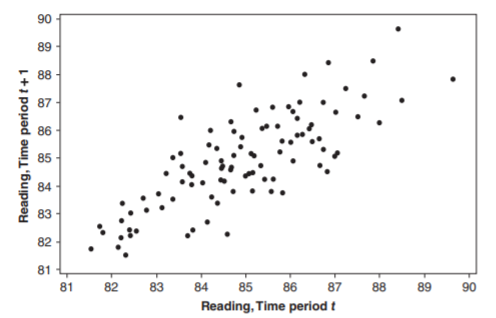
\includegraphics[width=70mm]{./corr}}
\caption{Datos correlacionados y no correlacionados}
\label{correlation}
\end{figure}

Las figuras \ref{correlation} (a) y \ref{correlation} (b) son diagramas de dispersión con un retraso $k=1$. Ambos diagramas de dispersión se construyeron trazando $y_{t+1}$ versus $y_{t}$. La figura \ref{correlation} (a)  exhibe poca estructura, ya que los pares trazados de observaciones adyacentes $y_{t}, y_{t+1}$ parecen no estar \textit{correlacionados}, es decir, el valor de $y$ en el período actual no proporciona ninguna información útil sobre el valor de $y$ que se observará en el próximo período. Por otro lado, en figura \ref{correlation}  (b), los pares de observaciones adyacentes $y_{t+1}, y_{t}$ están positivamente correlacionados, es decir, un valor pequeño de $y$ tiende a ser seguido en el siguiente período por otro valor pequeño de $y$, y un valor grande de $y$ tiende a ser seguido inmediatamente por otro valor grande de $y$.

La covarianza entre $y_{t}$ y su valor en otro período de tiempo, digamos, $y_{t+k}$ se llama \textit{autocovarianza} en el retraso $k$, definido por:
\begin{equation}
\gamma_{k} = \text{Cov}(y_{t},y_{t+k}) = E[(y_{t} - \mu)(y_{t+k} - \mu)].
\end{equation}

La colección de los valores de $\gamma_{k}$, $k = 0, 1, 2, ...$ se llama \textit{Función de autocovarianza}, donde la \textit{autocovarianza} en el retraso $k=0$ es la \textit{varianza} de la serie de tiempo, es decir, $\gamma_{0} = \sigma^{2}_{y}$, que es constante para una serie de tiempo estacionaria. Además, el coeficiente de autocorrelación en el intervalo $k$ para una serie temporal estacionaria se calcula como:
\begin{equation}
\rho_{k} = \frac{E[(y_{t} - \mu)(y_{t+k} - \mu)]}{\sqrt{E[(y_{t} - \mu)]^{2} E[(y_{t+k} - \mu)^{2}]}} = \frac{\text{Cov}(y_{t},y_{t+k})}{\text{Var}(y_{t})} = \frac{\gamma_{k}}{\gamma_{0}}.
\end{equation}

La colección de los valores de $\rho_{k}$, $k = 0, 1, 2, ...$ se llama \textit{Función de autocorrelación (ACF)}, donde $\rho_{0} = 1$. Además, el ACF es independiente de la escala de medición de la serie de tiempo. También, $\rho_{k} = \rho_{-k}$, es decir, el ACF es simétrico alrededor de cero, por lo que solo es necesario calcular la mitad positiva (o negativa).

Si una serie de tiempo tiene función de autocovarianza y media finita, se dice que es estacionaria de segundo orden (o débilmente estacionaria de orden dos). Si además, la distribución de probabilidad conjunta de las observaciones en todo momento es multivariante normal, entonces eso es suficiente para dar como resultado una serie de tiempo estrictamente estacionaria.

Es necesario estimar la autocovarianza y los ACF a partir de un momento de longitud finita, digamos, $y_{1}, y_{2}, ..., y_{t}$. La estimación habitual de la función de autocovarianza se calcula como:
\begin{equation}
c_{k} = \hat{\gamma_{k}} = \frac{1}{T} \sum_{t=1}^{T-k} (y_{t}-\overline{y})(y_{t+k}-\overline{y}), \ k=0, 1, ..., k,
\end{equation}

y el ACF es estimado por la función de autocorrelación de muestra (o muestra de ACF) calculada como:
\begin{equation}
r_{k} = \hat{\rho_{k}} = \frac{c_{k}}{c_{0}}, \ k=0, 1, ..., k.
\end{equation}

\subsection{Variograma}

A menudo en la práctica no hay una demarcación clara entre un proceso estacionario y uno no estacionario para muchas series de tiempo del mundo real. Por ello, una herramienta de diagnóstico adicional que es muy útil es el \textit{Variograma}.

Suponga que las observaciones de la serie de tiempo están representadas por $y_{t}$. El variograma $G_{k}$ mide las variaciones de las diferencias entre las observaciones que están separadas a una distancia $k$, en relación con la variación de las diferencias que están separadas por una unidad de tiempo. El variograma se define como:
\begin{equation}
G_{k} = \frac{\text{Var}(y_{t+k}-y_{t})}{\text{Var}(y_{t+1}-y_{t})}, k=1, 2, ...
\end{equation}

y los valores de $G_{k}$ se representan en función del retraso $k$. Si la serie temporal es estacionaria, resulta que:
\begin{equation}
G_{k} = \frac{1- \rho_{k}}{1-\rho_{1}},
\end{equation}

para una serie temporal estacionaria $\rho_{k} \rightarrow 0$ a medida que $k$ aumenta, por lo que cuando el variograma se traza contra el retraso $k$, $G_{k}$ alcanzará una asíntota $\frac{1}{(1 - \rho_{1})}$. Sin embargo, si la serie temporal no es estacionaria, $G_{k}$ aumentará monótonamente. 



\section{Métodos de Interpolación}

Sea $P_{n} = \{ p_{1}, p_{2}, ..., p_{n} \}, n \geq 2$ el conjunto de puntos muestrales (estaciones de monitoreo) en el espacio $\mathbb{R}^{2}$ o \textit{plano Euclideano}, etiquetados mediante las coordenadas $(x_{1}, y_{1}), ..., (x_{n}, y_{n})$. Los $n$ puntos son distintos en el sentido de que $(x_{i}, y_{i}) \neq (x_{j}, y_{j}) \ \forall p_{i}, p_{j} \in P_{n}$.


\begin{defn} \textbf{(Distancia Euclidiana)}. Sean $p$ y $p^{*}$ dos puntos arbitrarios en el plano Euclidiano con coordenadas $(x, y)$ y $(x^{*}, y^{*})$ respectivamente. Entonces, la \textit{distancia Euclidiana} entre $p$ y $p^{*}$ está dada por:
\begin{equation}
d(p, p^{*}) = \lVert p - p^{*} \rVert = \sqrt{ {(x-x^{*})}^{2} + {(y-y^{*})}^{2} }.
\end{equation} \end{defn}

\textbf{Nota:} Se considera a partir de ahora que se trabaja en el espacio Euclidiano con la \textit{métrica Euclidiana}.


\subsection{Determininistas}

La interpolación mediante métodos de interpolación deterministas indica los valores de un punto desconocido a través de una combinación ponderada linealmente de un conjunto de puntos conocidos (puntos de muestra). Los métodos de interpolacion deterministas suponen que la superficie que se interpola debe ser la de una variable dependiente de la ubicación. En esta sección se definen los métodos de interpolación deterministas que se utilizan en este trabajo y son: Diagramas de Voronoi, Funciones de Base Radial y el método de Distancia Inversa Ponderada.

\subsubsection{Diagramas de Voronoi}


\begin{defn} \textbf{(Diagrama de Voronoi (DV))}. Sea el conjunto $P_{\mathcal{V}}$ = $\{ p_{1}, p_{2}, ...,$ \\ $p_{n} \} \subset \mathbb{R}^{2}$, con $2 < n$ y $x_{i} \neq x_{j} \forall \ i, j$. Llamemos a la región dada por: 
\begin{equation}  
V(p_{i})= \{x : \parallel x-x_{i} \parallel \leq \parallel x-x_{j} \parallel, i \neq j \} \ \forall x_{i}, x_{j} \in P_{\mathcal{V}},
\label{pol_voronoi}
\end{equation}
como el \textit{Polígono de Voronoi} asociado a $p_{i}$ (o el Polígono de Voronoi de $p_{i}$ y al conjunto dado por
\begin{equation}
\mathcal{V} = \{ V(p_{1}),...,V(p_{n}) \}
\end{equation}
el \textit{Diagrama de Voronoi} generado por $P_{\mathcal{V}}$ (o el diagrama de Voronoi de $P_{\mathcal{V}}$). 
\label{voronoi}
\end{defn}

En la definición \ref{voronoi}, se observa de la ecuación \ref{pol_voronoi} que está definida en términos de desigualdad $(\leq)$, por lo que un polígono de Voronoi es un \textit{conjunto cerrado}. Dado que un polígono de Voronoi, éste contiene su frontera ($\partial V(p_{i})$) y podemos establecer las siguientes definiciones.

\begin{defn} \textbf{(Arista de Voronoi)}. Puesto que el diagrama de Voronoi contiene a su frontera $\partial V(p_{i})$, ésta puede consistir en segmentos de recta, semirectas o rectas infinitas, las cuales llamamos \textit{Aristas de Voronoi}. Denotamos a la arista de los polígonos de Voronoi $p_{i}$ y $p_{j}$ como $a (p_{i}, p_{j})$.
\end{defn}

\begin{defn} \textbf{(Vértice de Voronoi)}. Llamamos \textit{Vértice de Voronoi} a un punto extremo de una arista de Voronoi o se puede definir también como un punto compartido por tres o más polígonos de Voronoi. Denotamos a el vértice de Voronoi del polígono de Voronoi $p_{i}$ como $v_{i}$.
\end{defn}

\begin{defn} \textbf{(Red de Voronoi)}. El diagrama de Voronoi puede ser definido por la unión de las aristas de Voronoi, es decir, $\bigcup_{i=1}^{n} \partial V(p_{i})$  en lugar del conjunto $P_{\mathcal{V}}$. Llamamos a red \textit{(malla)}, conformada por la unión de aristas de Voronoi como la \textit{Red de Voronoi}.
\end{defn}





\subsubsection{Funciones de base radial}


\begin{defn} \textbf{(Funciones de Base Radial (FBR))}. Sea el conjunto $P_{\mathcal{F}} = \{ p_{1}, p_{2}, ..., p_{n} \} \subset \mathbb{R}^{2}$, con $x_{i} \neq x_{j} \forall \ i, j$. Llamemos \textit{Función de Base Radial} a una función perteneciente a una gran familia de interpoladores exactos que usan una \textit{ecuación básica} que es una función que depende de la distancia entre el punto interpolado y los puntos de muestreo $P_{\mathcal{F}}$. Los valores de predicción por una FBR se pueden expresar como la suma de dos componentes: 
\begin{equation} 
\hat{Z}(x)=\sum_{i=1}^{n} a_{i} f_{i}(x) + \sum_{j=1}^{n} b_{j} \psi(d_{j}), 
\end{equation}
donde $\psi(d_{j})$ es la ecuación básica que depende de la distacia $d_{j}$, donde $d_{j}$ es la distancia desde los puntos de muestra $P_{\mathcal{F}}$ a el punto interpolado $x$ y $f_{i}(x)$ es un polinomio de grado $< m$, con $m$ el número de puntos a interpolar. Los coeficientes $a_{i}$ y $b_{j}$ se calculan mediante la resolución del sistema de $n + m$ ecuaciones lineales, con $n$  el número de puntos conocidos $P_{\mathcal{F}}$ utilizados en la interpolación de la siguiente manera:
\begin{equation}
\hat{Z}(x_{k}) = \sum_{i=1}^{m} a_{i} f_{i}(x_{k}) + \sum_{j=1}^{n} b_{j} \psi(d_{jk}), \ k=1, 2, ..., n 
\end{equation}
\[ \sum_{j=1}^{n} b_{j} f_{k}(x_{j}) = 0, \ k= 1, 2, ..., m. \]
\end{defn}

En este trabajo de tesis se utilizan las siguientes clases de BRF para la interpolación de datos dispersos $n$-dimensionales a un dominio $m$-dimensional; Multicuadrática (M), Inversa multicuadrática (IM), Gaussiana (G), Lineal (L), Cúbica (C), Quíntica (Q) y Thin-plate splines (TPS). La función de base radial utilizada para cada caso da las siguientes expresiones:
\begin{itemize}
\item M: $\psi(d) = \sqrt{d^{2} + c^{2}}$
\item IM: $\psi(d) = \sqrt{d^{2} + c^{2}}^{-1}$
\item G: $\psi(d) = e^{-\sqrt{d^{2} + c^{2}}}$
\item L: $\psi(d) = d$
\item C: $\psi(d) = d^{3}$
\item Q: $\psi(d) = d^{5}$
\item TPS: $\psi(d) =  d^{2} + c^{2} \ln (cd)$,
\end{itemize}

donde $d$ es la distancia de los puntos muestra $P_{\mathcal{F}}$ a la ubicación de predicción $x$ y $c$ es un factor de suavizado.






\subsubsection{Distancia inversa ponderada}



\begin{defn} (\textbf{Distancia Inversa Ponderada (DIP)}). Sea el conjunto $P_{\mathcal{D}} = \{ p_{1}, p_{2}, ..., p_{n} \} \subset \mathbb{R}^{2}$, con $x_{i} \neq x_{j} \forall \ i, j$. Llamemos función de \textit{Distancia Inversa Ponderada} a una función de la forma:
\begin{equation}
\hat{Z}(x)= \frac{\sum_{i=1}^{n} w_{i}z_{i}}{\sum_{i=1}^{n} w_{i}}
\end{equation}
\[ w_{i}=d_{i}^{-u}, \]
donde $Z(x)$ es el valor predicho en el punto $x$, $Z_{i}$ es el valor del punto muestra $p_{i}$, $d_{i}$ es la distancia entre el punto $p_{i}$ y el punto $x$ y $w_{i}$ es el peso asignado al punto $p_{i}$.
\end{defn}

Los valores de mayor ponderación se asignan a valores más cercanos al punto interpolado. A medida que la distancia aumenta, el peso disminuye \citep{shepard}, y $u$ es el poder de ponderación que decide cómo disminuye el peso a medida que aumenta la distancia.





\subsection{Geoestadísticos}

La interpolación mediante métodos de interpolación geoestadísticos o probabilísticos se resumen en el método de interpolación \textit{Kriging}. La palabra Kriging (expresión anglosajona) proviene del nombre del geólogo sudafricano Danie G. Krige, cuyo trabajo aportó a la predicción de reservas de oro, realizados en la década de los años cincuentas y éste suele considerarse como el pionero en los métodos de interpolación geoespacial. 

Kriging encierra un conjunto de métodos de predicción espacial que se centran en la minimización del error cuadrático medio de predicción. Al igual que con DIP, el estimador de Kriging viene dado por una combinación lineal de los valores observados y los pesos. Dependiendo de las propiedades estocásticas de los campos aleatorios, se aplican diferentes tipos de Kriging. En esta sección se definen los métodos de interpolación geoestadísticos que se utilizan en este trabajo y son: Kriging Ordinario y Kriging Universal.



\subsubsection{Kriging Ordinario}

\begin{defn} (\textbf{Kriging Ordinario (KO)}). Sea el conjunto $P_{\mathcal{O}} = \{ p_{1}, p_{2}, ..., p_{n} \} \\ \subset \mathbb{R}^{2}$, con $x_{i} \neq x_{j} \forall \ i, j$. Supongase que se hacen mediciones de la variable de interés $Z$ en los puntos $p_{i} \in P_{\mathcal{O}} \forall i$, es decir, se tienen $Z(x_{1}), ..., Z(x_{n})$, y se desea predecir el punto $Z(x^{*})$, en el punto $x^{*}\notin P_{\mathcal{O}}$ donde no hubo medición. Llamemos \textit{Kriging Ordinario} al método que predice con una combinación lineal las $n$ variables aleatorias como:
\begin{equation}
\hat{Z}(x^{*}) = \lambda_{1} Z(x_{1}) + \lambda_{2} Z(x_{2}) + ... + \lambda_{n} Z(x_{n}) = \sum_{i=1}^{n} \lambda_{i} Z(x_{i}), \end{equation} donde $\lambda_{i}$ representan los pesos de los valores de los puntos muestrales y $x_{i}$ son los valores observados en los puntos $p_{i}$.
\end{defn}

Dichos pesos se calculan en función de la distancia entre los puntos muestrales $(P_{\mathcal{O}})$ y el punto predicho $x^{*}$. La suma de los pesos debe ser igual a uno para que la esperanza del predictor sea igual a la esperanza de la variable. Esto último se conoce como \textit{propiedad de insesgamiento}. 

Estadísticamente la propiedad de insesgamiento es:
\[ E\left[ \sum_{i=1}^{n} \lambda_{i} Z(x_{i}) \right] = m, \]
\[ \sum_{i=1}^{n}  \lambda_{i} E[Z(x_{i})] = m, \]
\[ \sum_{i=1}^{n}  \lambda_{i} m = m, \]
\[m \sum_{i=1}^{n}  \lambda_{i} = m \Rightarrow \sum_{i=1}^{n}  \lambda_{i} = 1.\]

Se dice que $\hat{Z}(x^{*})$ es el mejor predictor lineal en este caso, ya que los pesos se obtienen de tal manera que minimicen la varianza del error de predicción, es decir, que minimicen la expresión dada por:
\begin{equation}
V[ \hat{Z}(x^{*}) - Z(x^{*})].
\end{equation}
Esta característica es distintiva de los métodos Kriging, ya que métodos de interpolación deterministas no garantizan
varianza mínima de predicción \citep{samper}. La estimación de los pesos se obtiene resolviendo:
\[\text{Min.} \ \ V[ \hat{Z}(x^{*}) - Z(x^{*})] \]
\[ \text{s. a.} \ \ \sum_{i=1}^{n}  \lambda_{i} = 1. \] 


Los pesos de KO se derivan de la \textit{función de semivariancia}. Los parámetros de la función de semivariancia y el \textit{efecto de pepita} se pueden estimar mediante una \textit{función de semivariación empírica} \citep{webster}. Un estimador imparcial de la función de semivariancia es la mitad de la diferencia cuadrática promedio entre los valores de datos dado por:
\begin{equation}
\gamma (h) = \frac{1}{2N(h)} \sum_{i=1}^{N(h)} [z(x_{i}) - z(x_{i} +h)]^{2}, 
\end{equation}
donde $\gamma (h)$ es el valor de semivariancia en el intervalo de distancia $h$, $N(h)$ es el número de pares de muestras dentro del intervalo de distancia $h$ y $z(x_{i} + h)$ y $z(x_{i})$ son valores de muestra en dos puntos separados por el intervalo de distancia $h$.




\subsubsection{Kriging Universal}

En los supuestos de KO se ha asumido que la variable es estacionaria, pero en la mayoría de los casos la variable no satisface esta condición y se caracteriza por exhibir una tendencia. Para tratar este tipo de variables es frecuente descomponer la variable $Z(x)$ en la suma de la tendencia, tratada como una función determinística más una componente estocástica estacionaria de media cero.

\begin{defn} (\textbf{Kriging Universal (KU)}). Sea el conjunto $P_{\mathcal{U}} = \{ p_{1}, p_{2}, ..., p_{n} \} \subset \mathbb{R}^{2}$, con $x_{i} \neq x_{j} \forall \ i, j$. Llamemos \textit{Kriging Universal} al método que predice como la suma de la tendencia, tratada a manera de una función determinística más una componente estocástica estacionaria de media cero las $n$ variables aleatorias, por ejemplo:
\begin{equation}
\hat{Z}(x) = m(x) + \epsilon(x),
\end{equation}
con $E[\epsilon(x)] = 0$, $V[\epsilon(x)] = \sigma^{2}$ y $E[Z(x)] = m(x)$.
\end{defn}

La tendencia puede expresarse mediante:
\[ m(x) = \sum_{l=1}^{p} a_{l} f_{l} (x), \]
donde las funciones $f_{l}(x)$ son conocidas y $p$ es el número de términos empleados para ajustar $m(x)$. Por lo tanto, el predictor de KU se define como:
\begin{equation}
\hat{Z} (x^{*}) = \sum_{i=1}^{n} \lambda_{i} Z(x_{i}).
\end{equation} 

 

























\chapter{Metodología y Experimentación}

Este capítulo comienza abordando los temas explicados en el marco teórico y su implementación a los datos en este trabajo de tesis. Primero, se muestra en análisis estadístico de los datos, número de variables, cantidad de registros, cantidad de datos faltantes y cantidad de datos atípicos o anómalos; acompañado de descripciones visuales como series de tiempo por estación de cada variable, seguido de matrices de correlación entre estaciones por variable. Después, se menciona cómo se eliminan datos no deseables y se acompletan dichos registros para así, por último, tener una base de datos decente para llevar a cabo la experimentación y obtención de resultados discutidos en el capítulo siguiente.



\section{Análisis Estadístico y Limpieza de la Base de Datos}

Las estaciones de monitoreo indican las tendencias puntuales en la calidad del aire, pero sólo representan microambientes alrededor de ellas, por lo que se utilizan {\em métodos de interpolación espacial} para calcular los niveles de contaminantes en los lugares donde no hay estaciones de monitoreo.

La interpolación es el proceso de predecir valores en sitios sin muestrear. Los métodos de interpolación espacial incorporan información sobre la posición geográfica de los puntos de muestra, de modo que los puntos más cercanos entre sí tienen una mayor correlación y similitud que los que están más lejos. En este trabajo se evalúan los siguientes métodos de interpolación: Diagramas de Voronoi (DV), Distancia Inversa Ponderada (DIP), Funciones de Base Radial (FBR), Kriging Ordinario (KO) y Kriging Universal (KU).

La recolección de los datos se hace a partir del promedio de mediciones por hora. La base de datos cuenta con lo siguiente:\begin{itemize}
\item Trece estaciones de monitoreo.
\item 1,542,696 mediciones del promedio por hora (desde 1993-01-01 00:00:00 hrs. hasta 2018-12-31 23:00:00 hrs.).
\item Mediciones de quince variables por estación.
\end{itemize}
Luego se cuenta el número de datos faltantes en la base de datos por variable. 
\begin{table}[H]
\centering
\caption{Contaminantes y variables que recopilan las estaciones de monitoreo del SIMA con los nombres correspondientes de las variables en el código fuente \citep{sernagit}}
\begin{adjustbox}{max width=0.9\textwidth}
\begin{tabular}{|c|c|r|}
\hline
Variable &Nomenclatura MEEAMM  &Cantidad de \texttt{NaN} \\ \hline
Tiempo & timestamp   & 0              \\ \hline
\begin{tabular}[c]{@{}l@{}}Monóxido de Carbono\end{tabular}  & CO          & 253,474         \\ \hline
Óxido Nítrico    & NO          & 410,737         \\ \hline
\begin{tabular}[c]{@{}l@{}}Bióxido de Nitrógeno\end{tabular}  & NO$_{2}$         & 412,339         \\ \hline
\begin{tabular}[c]{@{}l@{}}Óxidos de Nitrógeno\end{tabular}  & NO$_{X}$         & 413,766         \\ \hline
Ozono  & O$_{3}$          & 305185         \\ \hline
\begin{tabular}[c]{@{}l@{}}Partículas menores a 10 micras\end{tabular}  & PM$_{10}$        & 159,985         \\ \hline
\begin{tabular}[c]{@{}l@{}}Partículas menores a 2.5 micras\end{tabular} & PM$_{2.5}$       & 1,014,253        \\ \hline
\begin{tabular}[c]{@{}l@{}}Presión Barométrica\end{tabular}  & pressure    & 610,362         \\ \hline
\begin{tabular}[c]{@{}l@{}}Precipitación Pluvial\end{tabular} & rainfall    & 489,331         \\ \hline
\begin{tabular}[c]{@{}l@{}}Humedad Relativa\end{tabular}  & humidity    & 550,968         \\ \hline
\begin{tabular}[c]{@{}l@{}}Bióxido de Azufre\end{tabular}  & SO$_{2}$         & 343,180         \\ \hline
Radiación Solar  & solar       & 675,701         \\ \hline
\begin{tabular}[c]{@{}l@{}}Temperatura Ambiental\end{tabular} & temperature & 109,143         \\ \hline
\begin{tabular}[c]{@{}l@{}}Velocidad del Viento\end{tabular} & velocity    & 109,590         \\ \hline
\begin{tabular}[c]{@{}l@{}}Dirección del Viento\end{tabular} & direction   & 178,126         \\ \hline
Total    &     & 7,554,588      \\  \hline
\end{tabular}
\end{adjustbox}
\end{table}


\begin{figure}[H]
\centering
\subfigure[Cantidad de datos conocidos y datos desconocidos por variable] {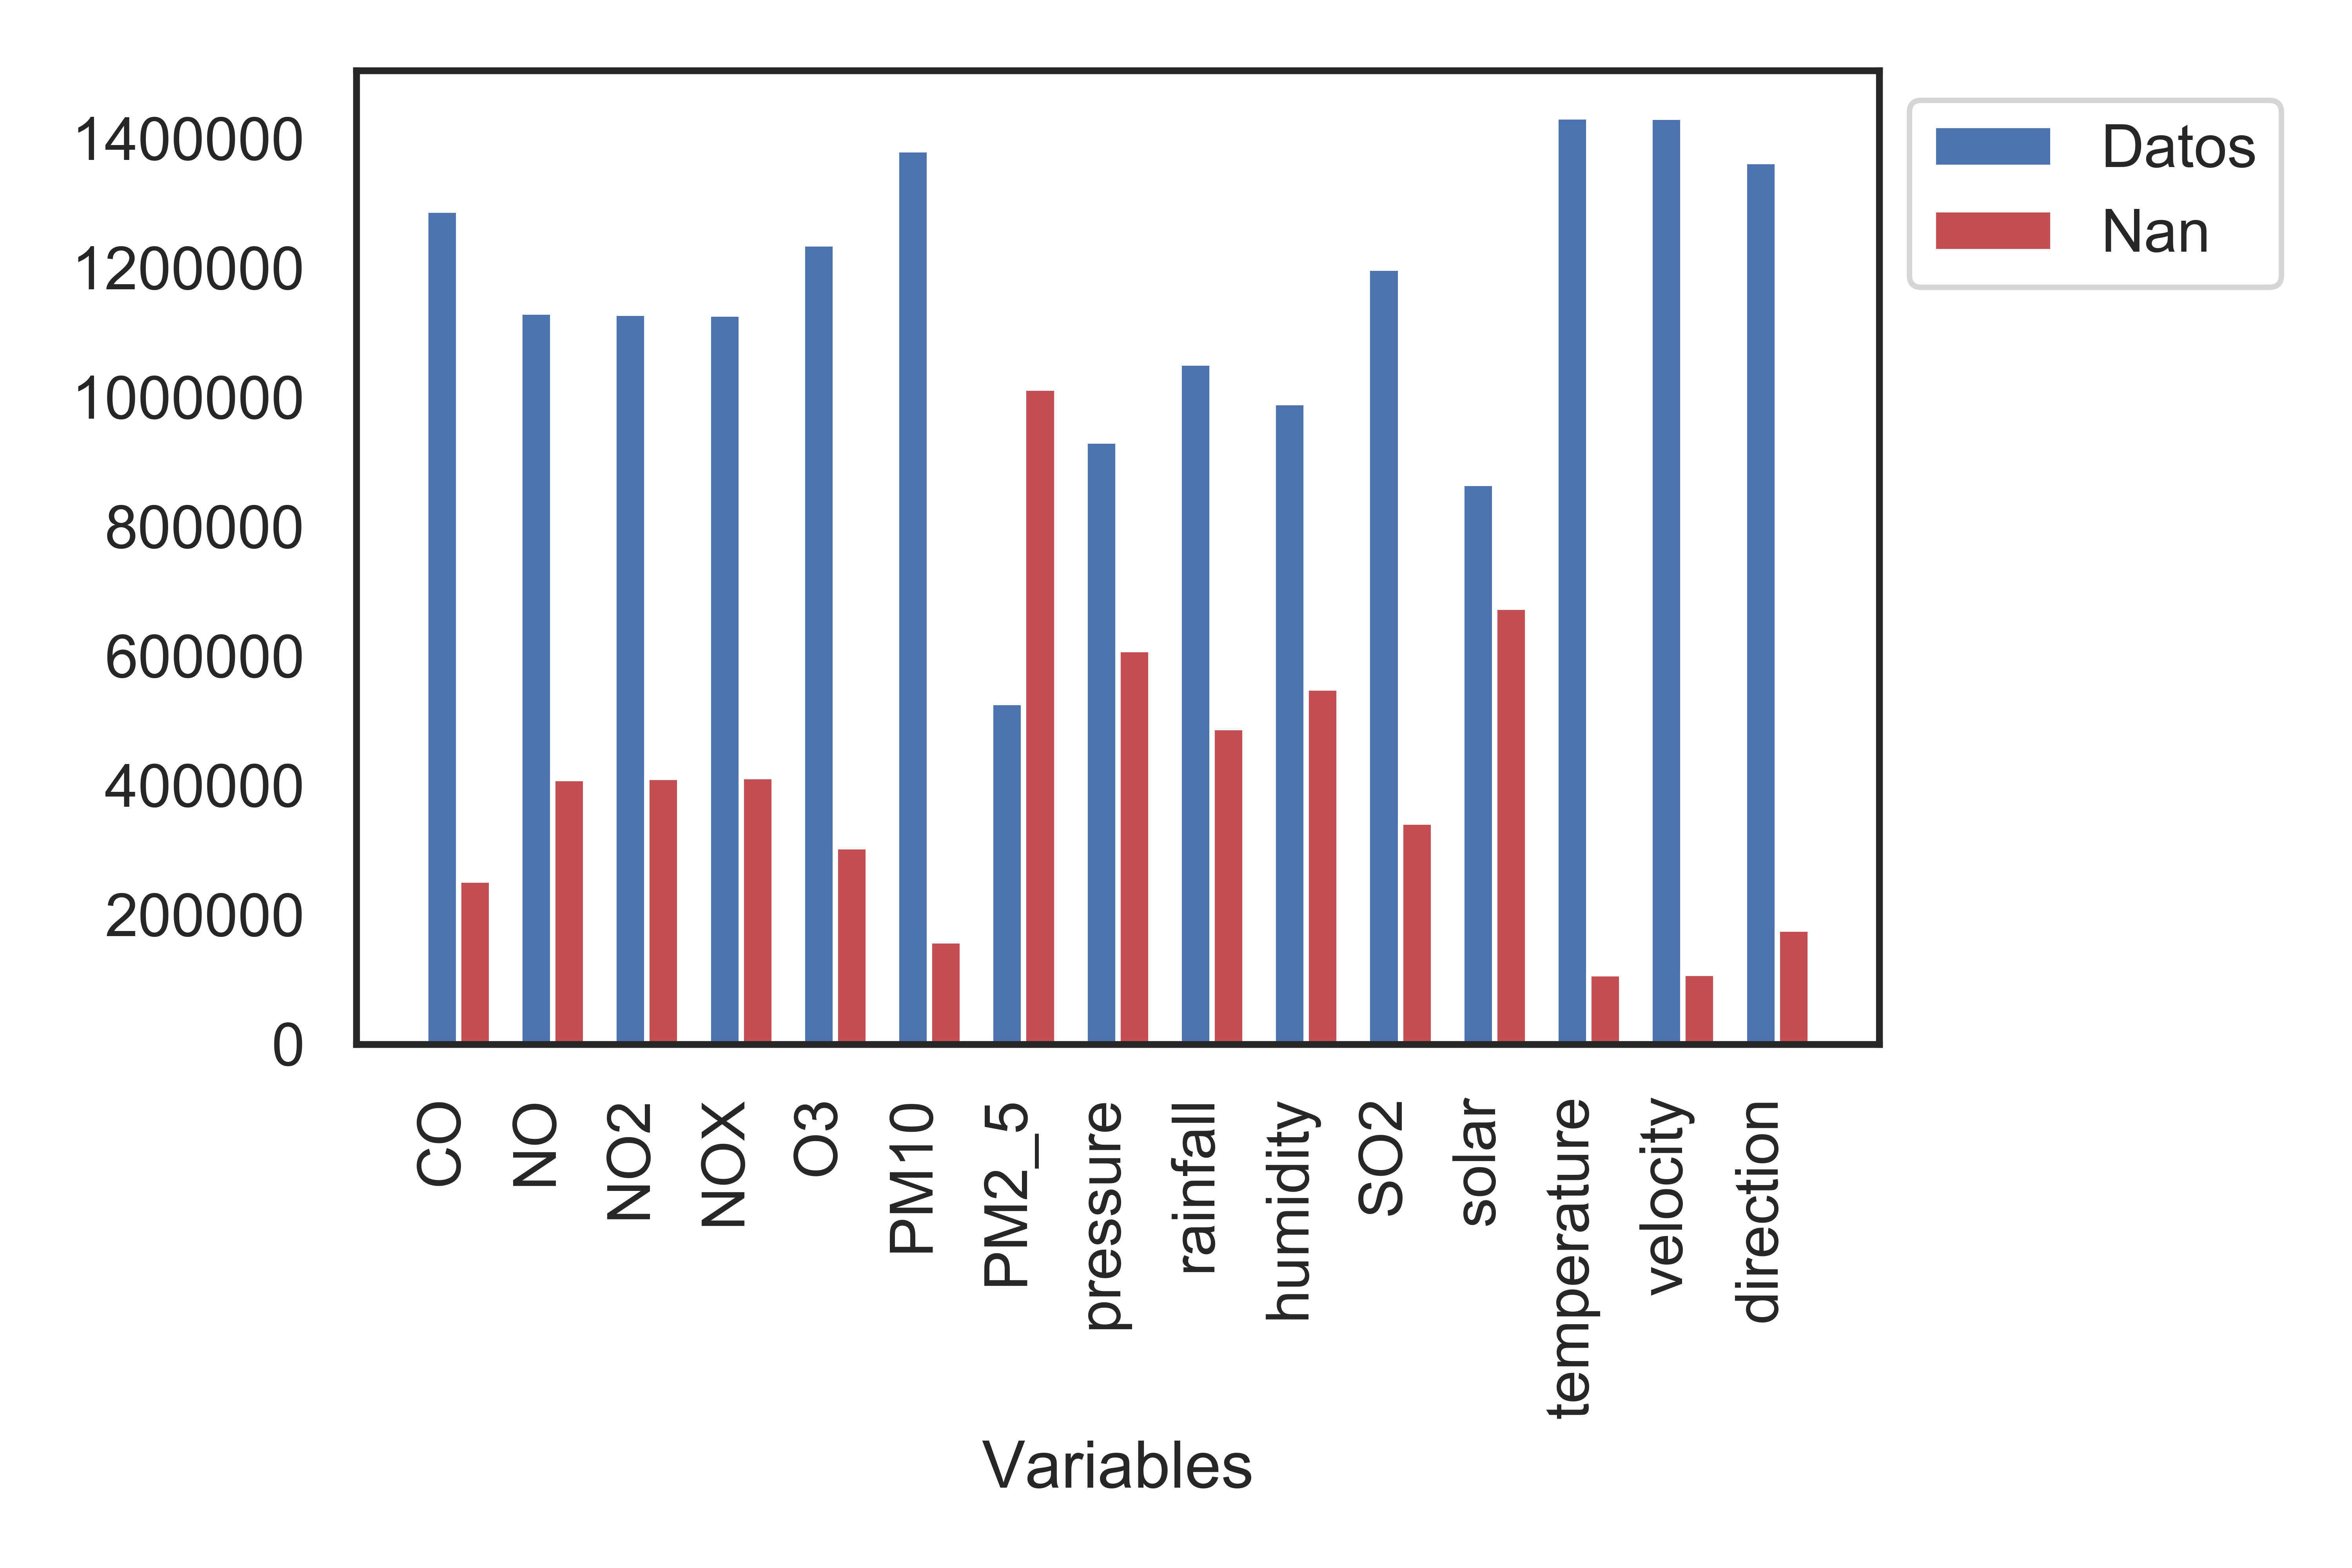
\includegraphics[width=72.5mm]{./BarPlot_All_2}}
\subfigure[Porcentaje de datos conocidos y datos desconocidos por variable]{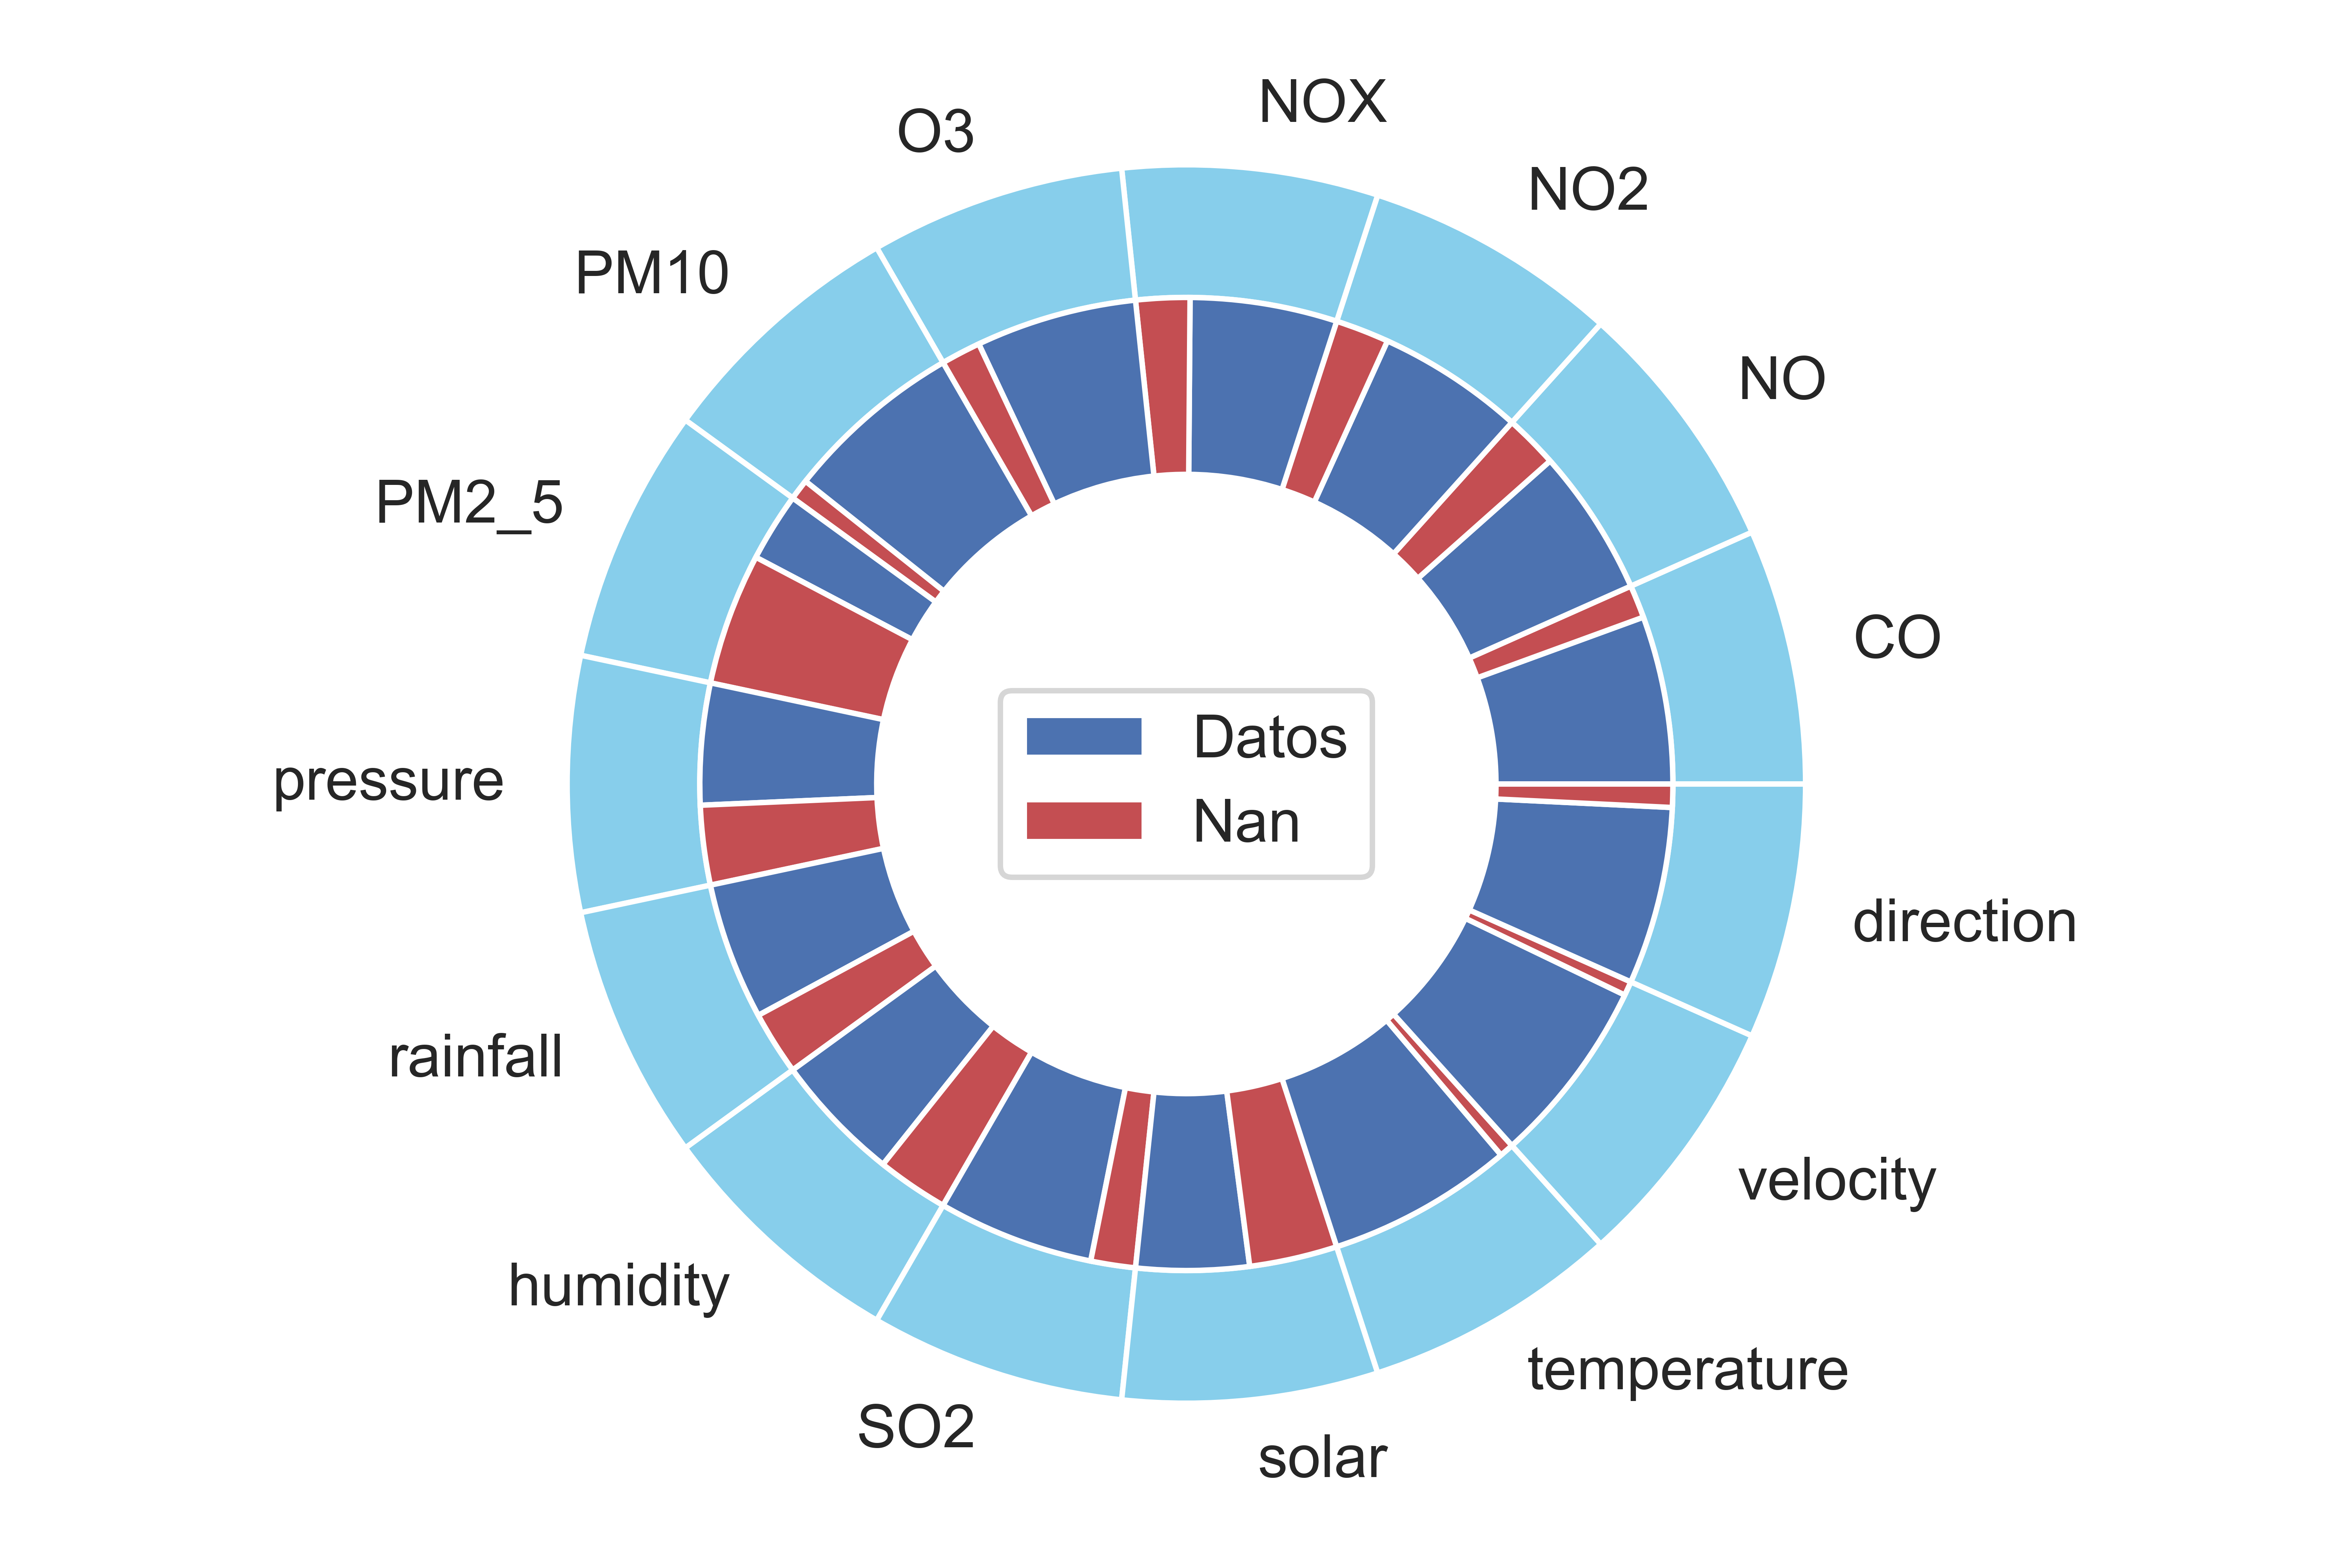
\includegraphics[width=72.5mm]{./BarPie}}
\subfigure[Porcentaje de datos conocidos y datos desconocidos por variable]{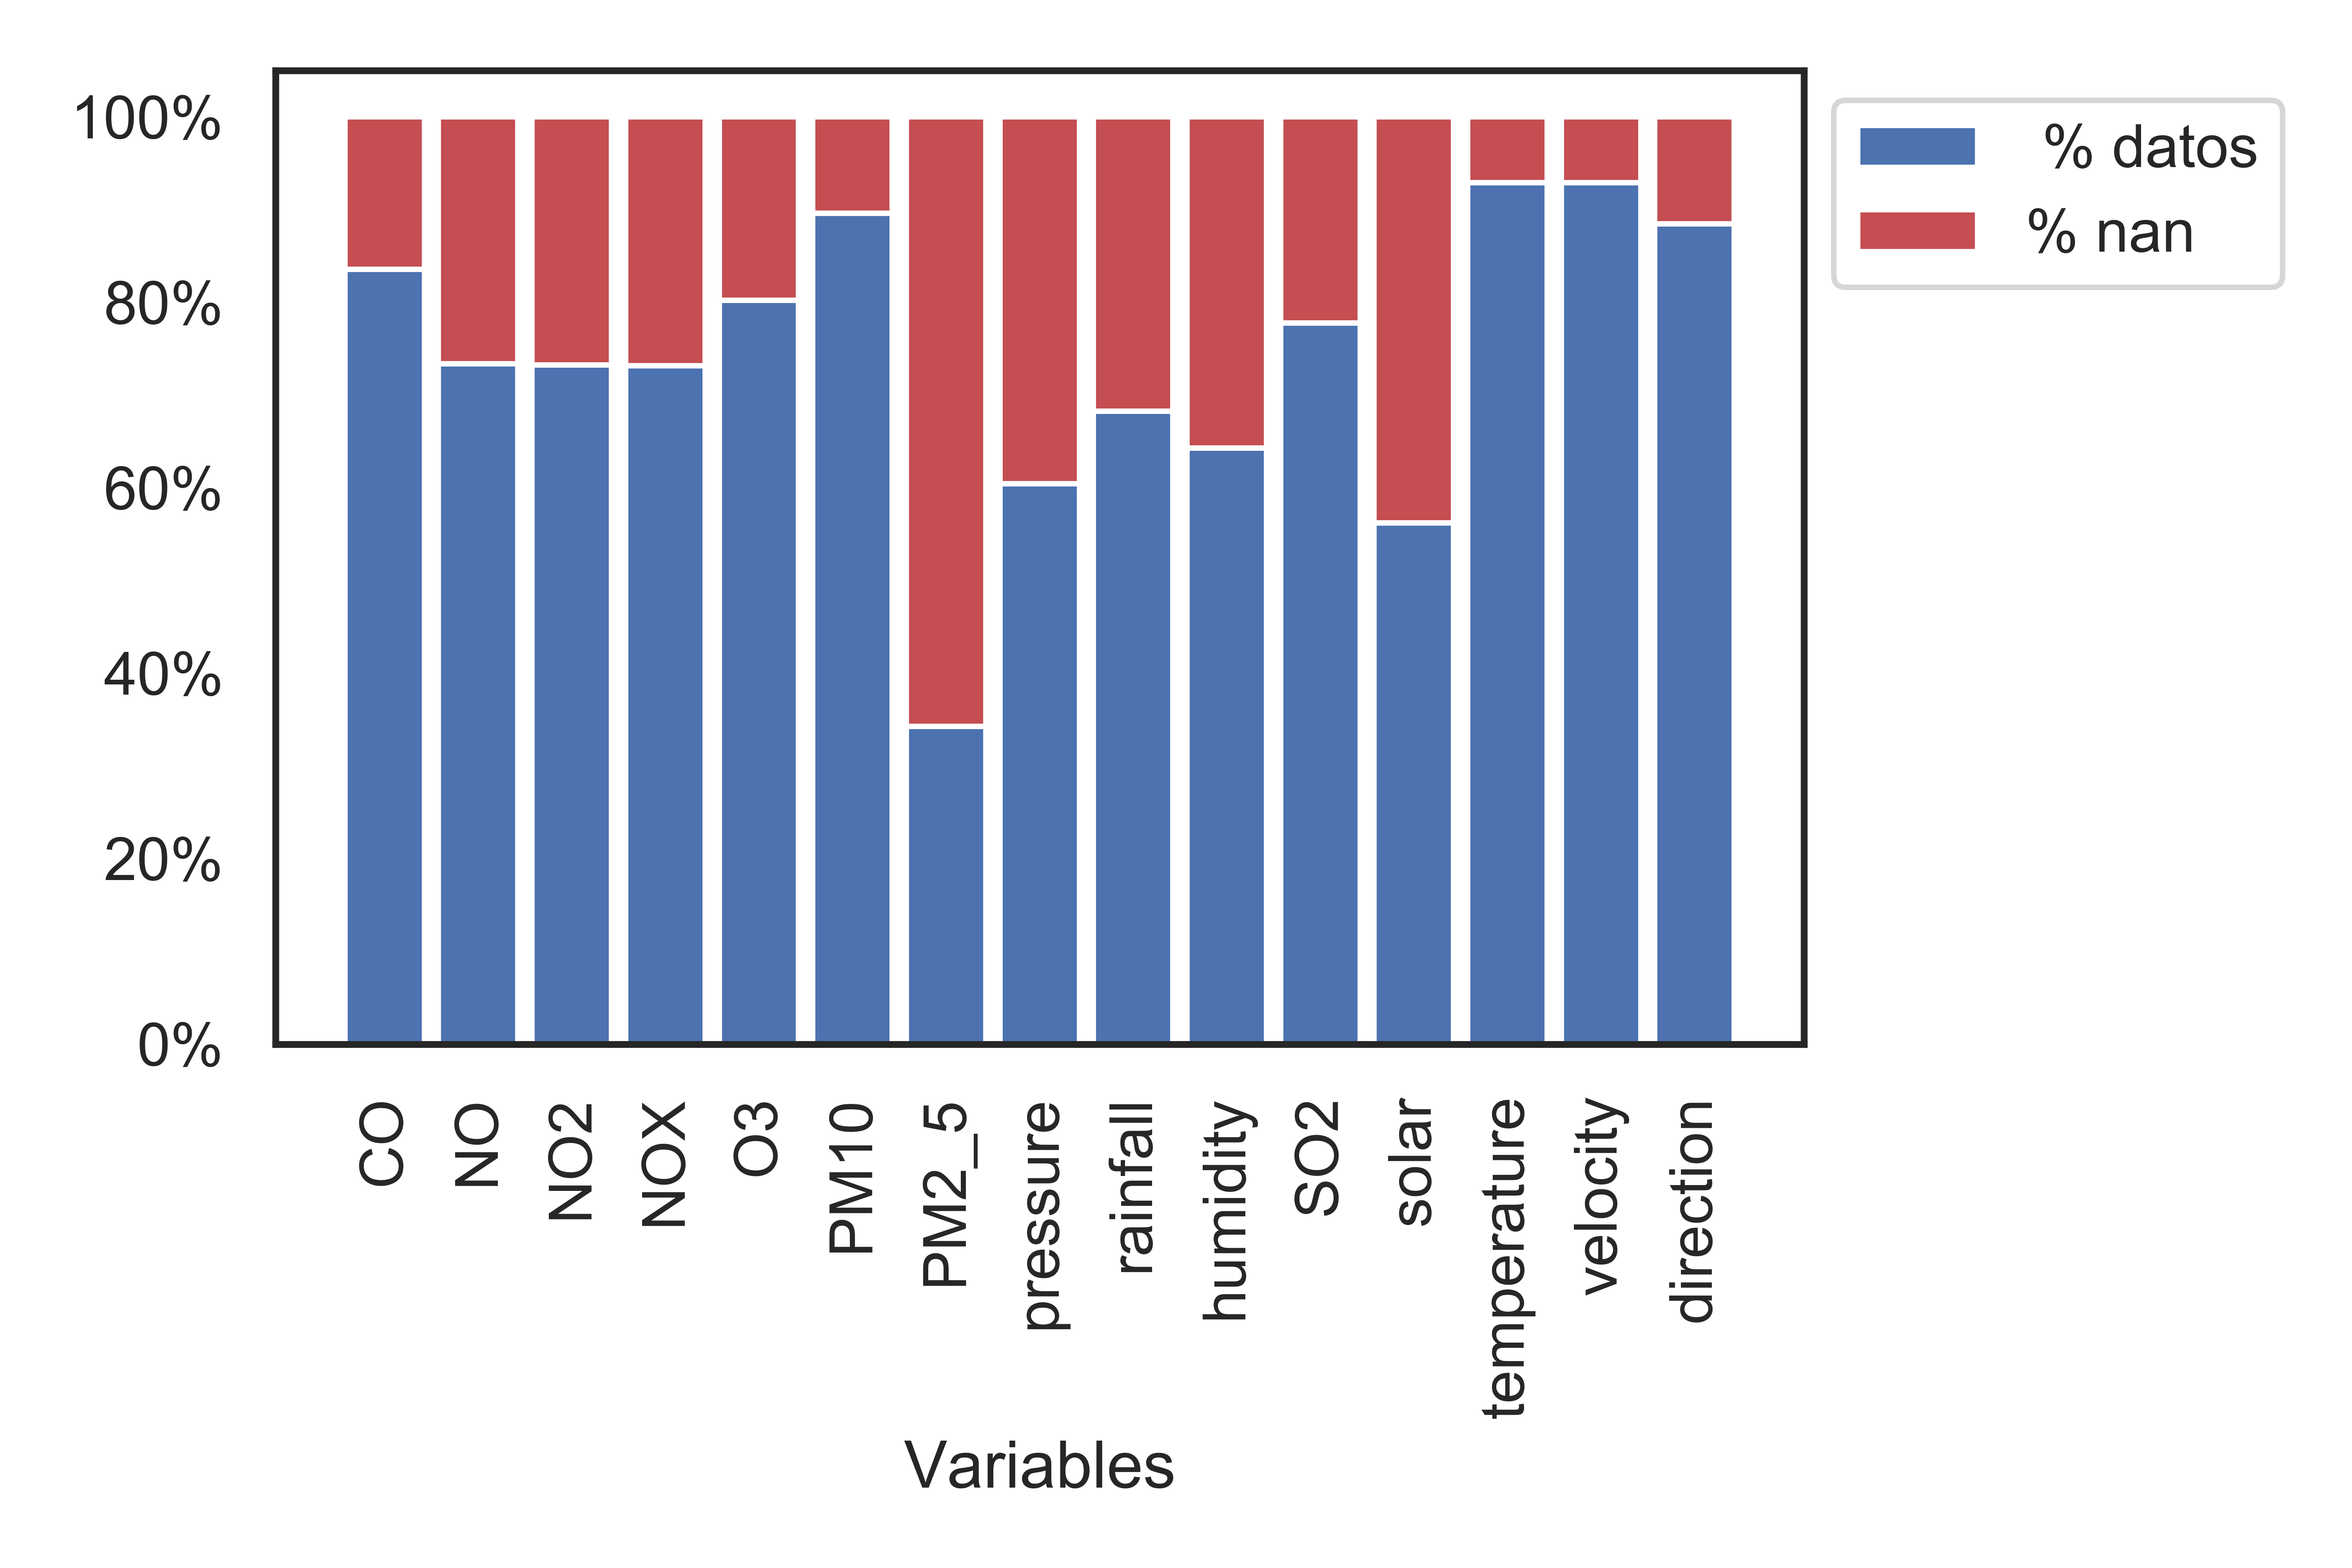
\includegraphics[width=72.5mm]{./BarPlot_All}}
\subfigure[Porcentaje de datos conocidos y datos desconocidos]{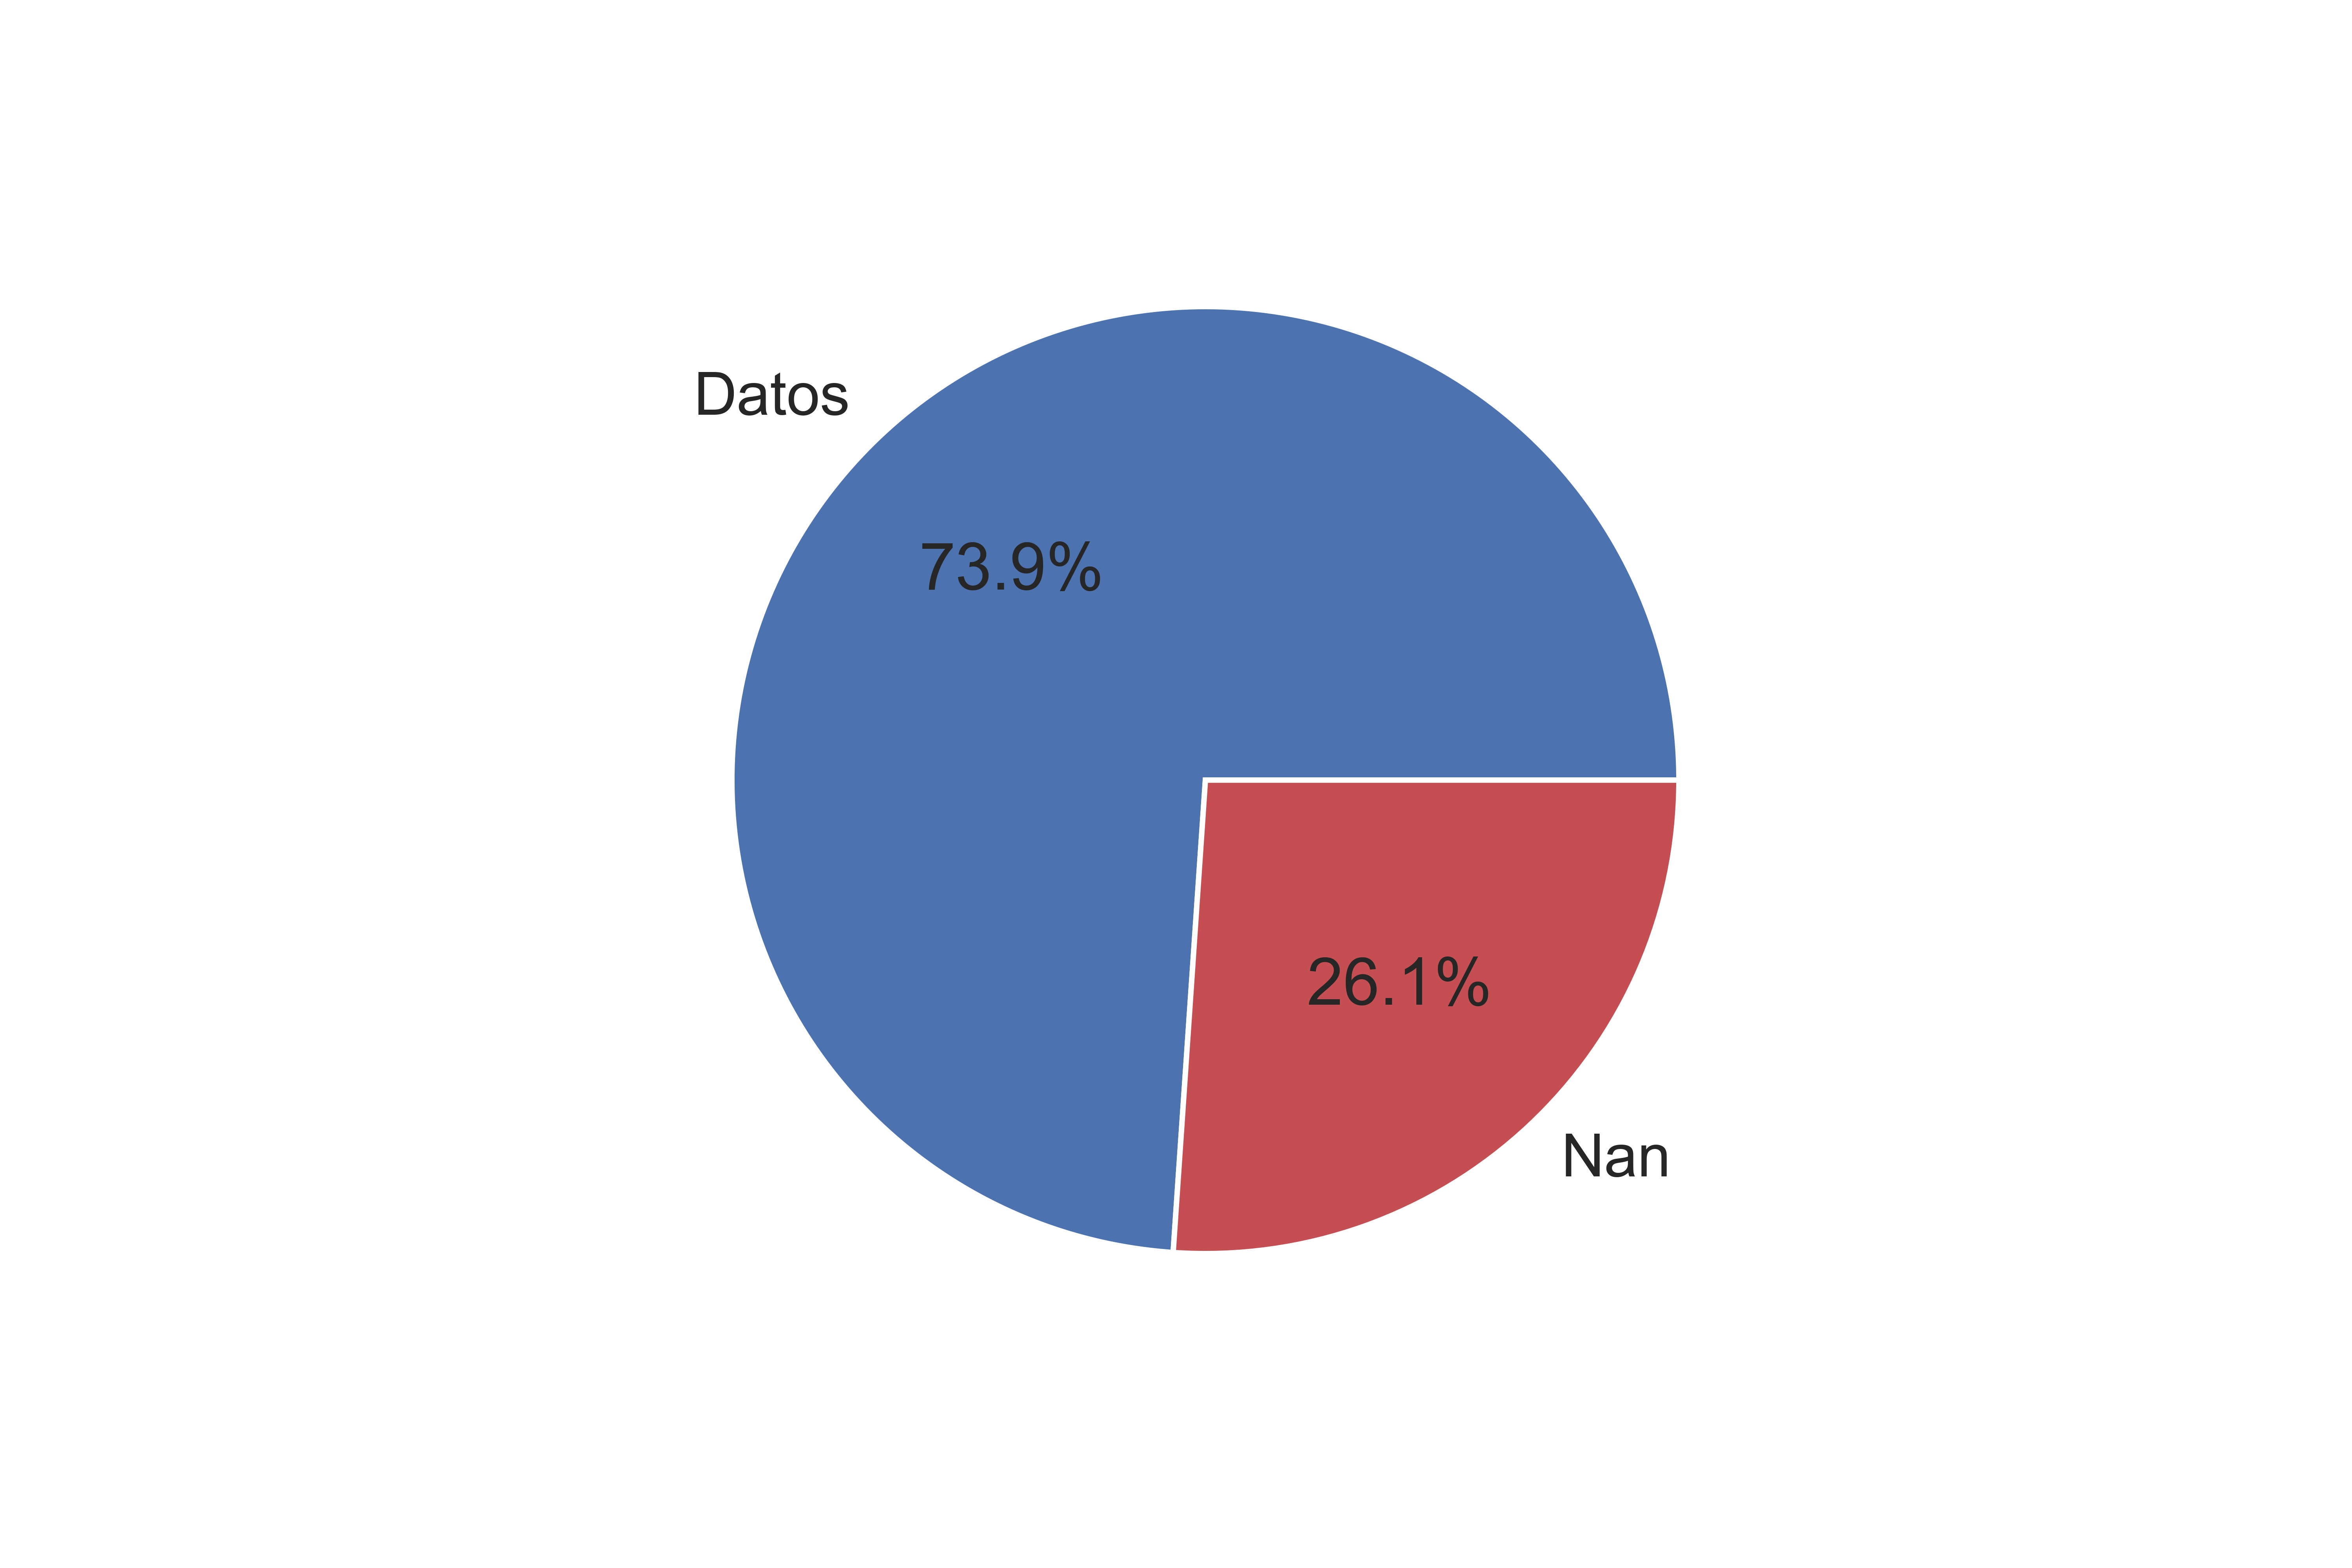
\includegraphics[width=72.5mm]{./BarPie_2}}
\caption{Datos conocidos y desconocidos (NaN) registrados por SIMA}
\label{figure1}
\end{figure}

De las quince variables con las que cuenta SIMA, que son: CO, NO, NO$_{2}$, NO$_{X}$, O$_{3}$, PM$_{10}$, PM$_{2.5}$, {\em Presión atmosférica, Precipitación pluvial, Humedad relativa}, SO$_{2}$, {\em Radiación solar, Temperatura ambiental, Velocidad del viento} y \textit{Dirección del viento}; se analizan cada una por individual. Lo primero que se hace es seleccionar los datos desde el año 2016, ya que algunas estaciones fueron puestas a trabajar hasta el año 2017; para recopilar la información de las variables en estas estaciones se hace el promedio de las estaciones más cercanas sin valores registrados para, posteriormente asignárselos.

Después de identificar la cantidad de datos faltantes, se prosigue con los valores que no son faltantes pero son no permitidos por estar fuera del rango de medición, esto es, el valor existe, aunque el valor de la medición fue provocado por una falla en el sensor de la estación de monitoreo. Los valores mínimos y máximos para cada variable se muestran en la tabla \ref{permitidos}. 

\begin{table}[H]
\centering
\caption{Valores fuera de rango por falla en analizadores y sensores de los diferentes parámetros en las estaciones de monitoreo atmosférico}
\begin{adjustbox}{max width=0.9\textwidth}
\begin{tabular}{|c|c|c|}
\hline
Parámetro &\multicolumn{2}{|c|}{Valores no permitidos}  \\ \hline
 &Menor a la lectura &Mayor a la lectura    \\ \hline
Partículas menores a 10 micras &2 &850\\
Partículas menores a 2.5 micras &2 &850\\
Ozono &1 &200\\   
Óxido Nítrico &1 &350\\ 
Bióxido de Nitrógeno &1 &150\\
Oxídos de Nitrógeno &1 &350\\
Bióxido de Azufre &1 &200\\
Monóxido de Carbono &0.05 &15\\
Temperatura ambiental &-15 &50\\
Precipitación pluvial &0 &---\\
Humedad relativa &0 &100 \\
Presión barométrica &650 &750 \\
Radiación solar &0 &1.2 \\
Velocidad del ciento &0 &60 \\
Dirección del viento &0 &360\\ \hline
\end{tabular}
\end{adjustbox}
\label{permitidos}
\end{table}

Después de identificar los valores faltantes y los valores no permitidos, se eliminan de la base de datos. Para completar los registros eliminados lo que se hace es interpolar los datos mediante la función \texttt{interpolate} con el método \texttt{time} cuando el valor fue un valor no permitido,  ya que la función \texttt{interpolate} consiste en seleccionar los valores al tiempo $t-1$ y al tiempo $t+1$ para asignar un valor en el registro al tiempo $t$ mediante una interpolación lineal. Para el caso de las estaciones en las que no se cuenta con información al tiempo $t-1$ y $t+1$, pues no se encontraban en operación la estación, lo que se hace es calcular el promedio por variable de las estaciones más cercanas a la estación que aún no está en operación, asignándole el valor promedio calculado hora a hora.


\subsection{Monóxido de Carbono (CO)} 
\begin{figure}[H]
\centering
\subfigure[Serie de tiempo de CO original] {\includegraphics[width=7cm, height=15cm]{./Serie_Nans_CO}}
\subfigure[Serie de tiempo de CO rellenando datos desconocidos]{\includegraphics[width=7cm, height=15cm]{./Serie_CO}}
\caption{Series de tiempo de CO desde 2016 hasta 2018}
\label{serieCO}
\end{figure}

La variable CO presenta datos faltantes durante intervalos de tiempo en los tres años seleccionados (ver figura \ref{serieCO} (a)), tales valores se completan haciendo el promedio de las estaciones cercanas a la estación con los datos faltantes  y se asigna el valor promedio a ésta, se puede apreciar en la figura \ref{serieCO} (b) que ya todas la estaciones cuentan con los valores en los tres años seleccionados, además se puede apreciar que la serie de tiempo es estacionaria, pues parece variar en torno a una media fija.

\begin{figure}[H]
\centering
\subfigure[Histograma de CO por estación] {\includegraphics[width=15cm, height=10cm]{./Histogram__2_CO_3}}
\subfigure[Histograma de CO]{\includegraphics[width=12cm, height=5cm]{./Histogram__2_CO_2}}
\caption{Histogramas de CO}
\label{histCO}
\end{figure}

La figura \ref{serieCO} muestra los gráficos de series de tiempo para la variable CO por estación y la figura \ref{histCO} muestra los histogramas de los datos por estación de la variable CO. De la figura \ref{serieCO} se puede observar que si bien las trece series de tiempo muestran características muy similares, es decir, son parecidas en estacionariedad en el tiempo, los histogramas de la figura \ref{histCO} son diferentes entre algunas estaciones, ya que el histograma resume los datos a través de la dimensión del tiempo, y al hacerlo, se pierden las características clave de los datos que dependen del tiempo.

\begin{figure}[H]
\centering
\includegraphics[width=12cm, height=10cm]{./Corr_CO_CO}
\caption{Matriz de correlación de CO entre estaciones}
\label{corrCOCO}
\end{figure}

La figura \ref{corrCOCO} muestra que la variable CO se correlaciona positivamente alto (correlaciones mayores a 0.2) entre la mayoría de las estaciones, pues la estación Sureste 2 muestra correlaciones bajas (correlaciones menores a 0.2) contra las estaciones Noroeste, Sur y Sureste 3.

\begin{figure}[H]
\centering
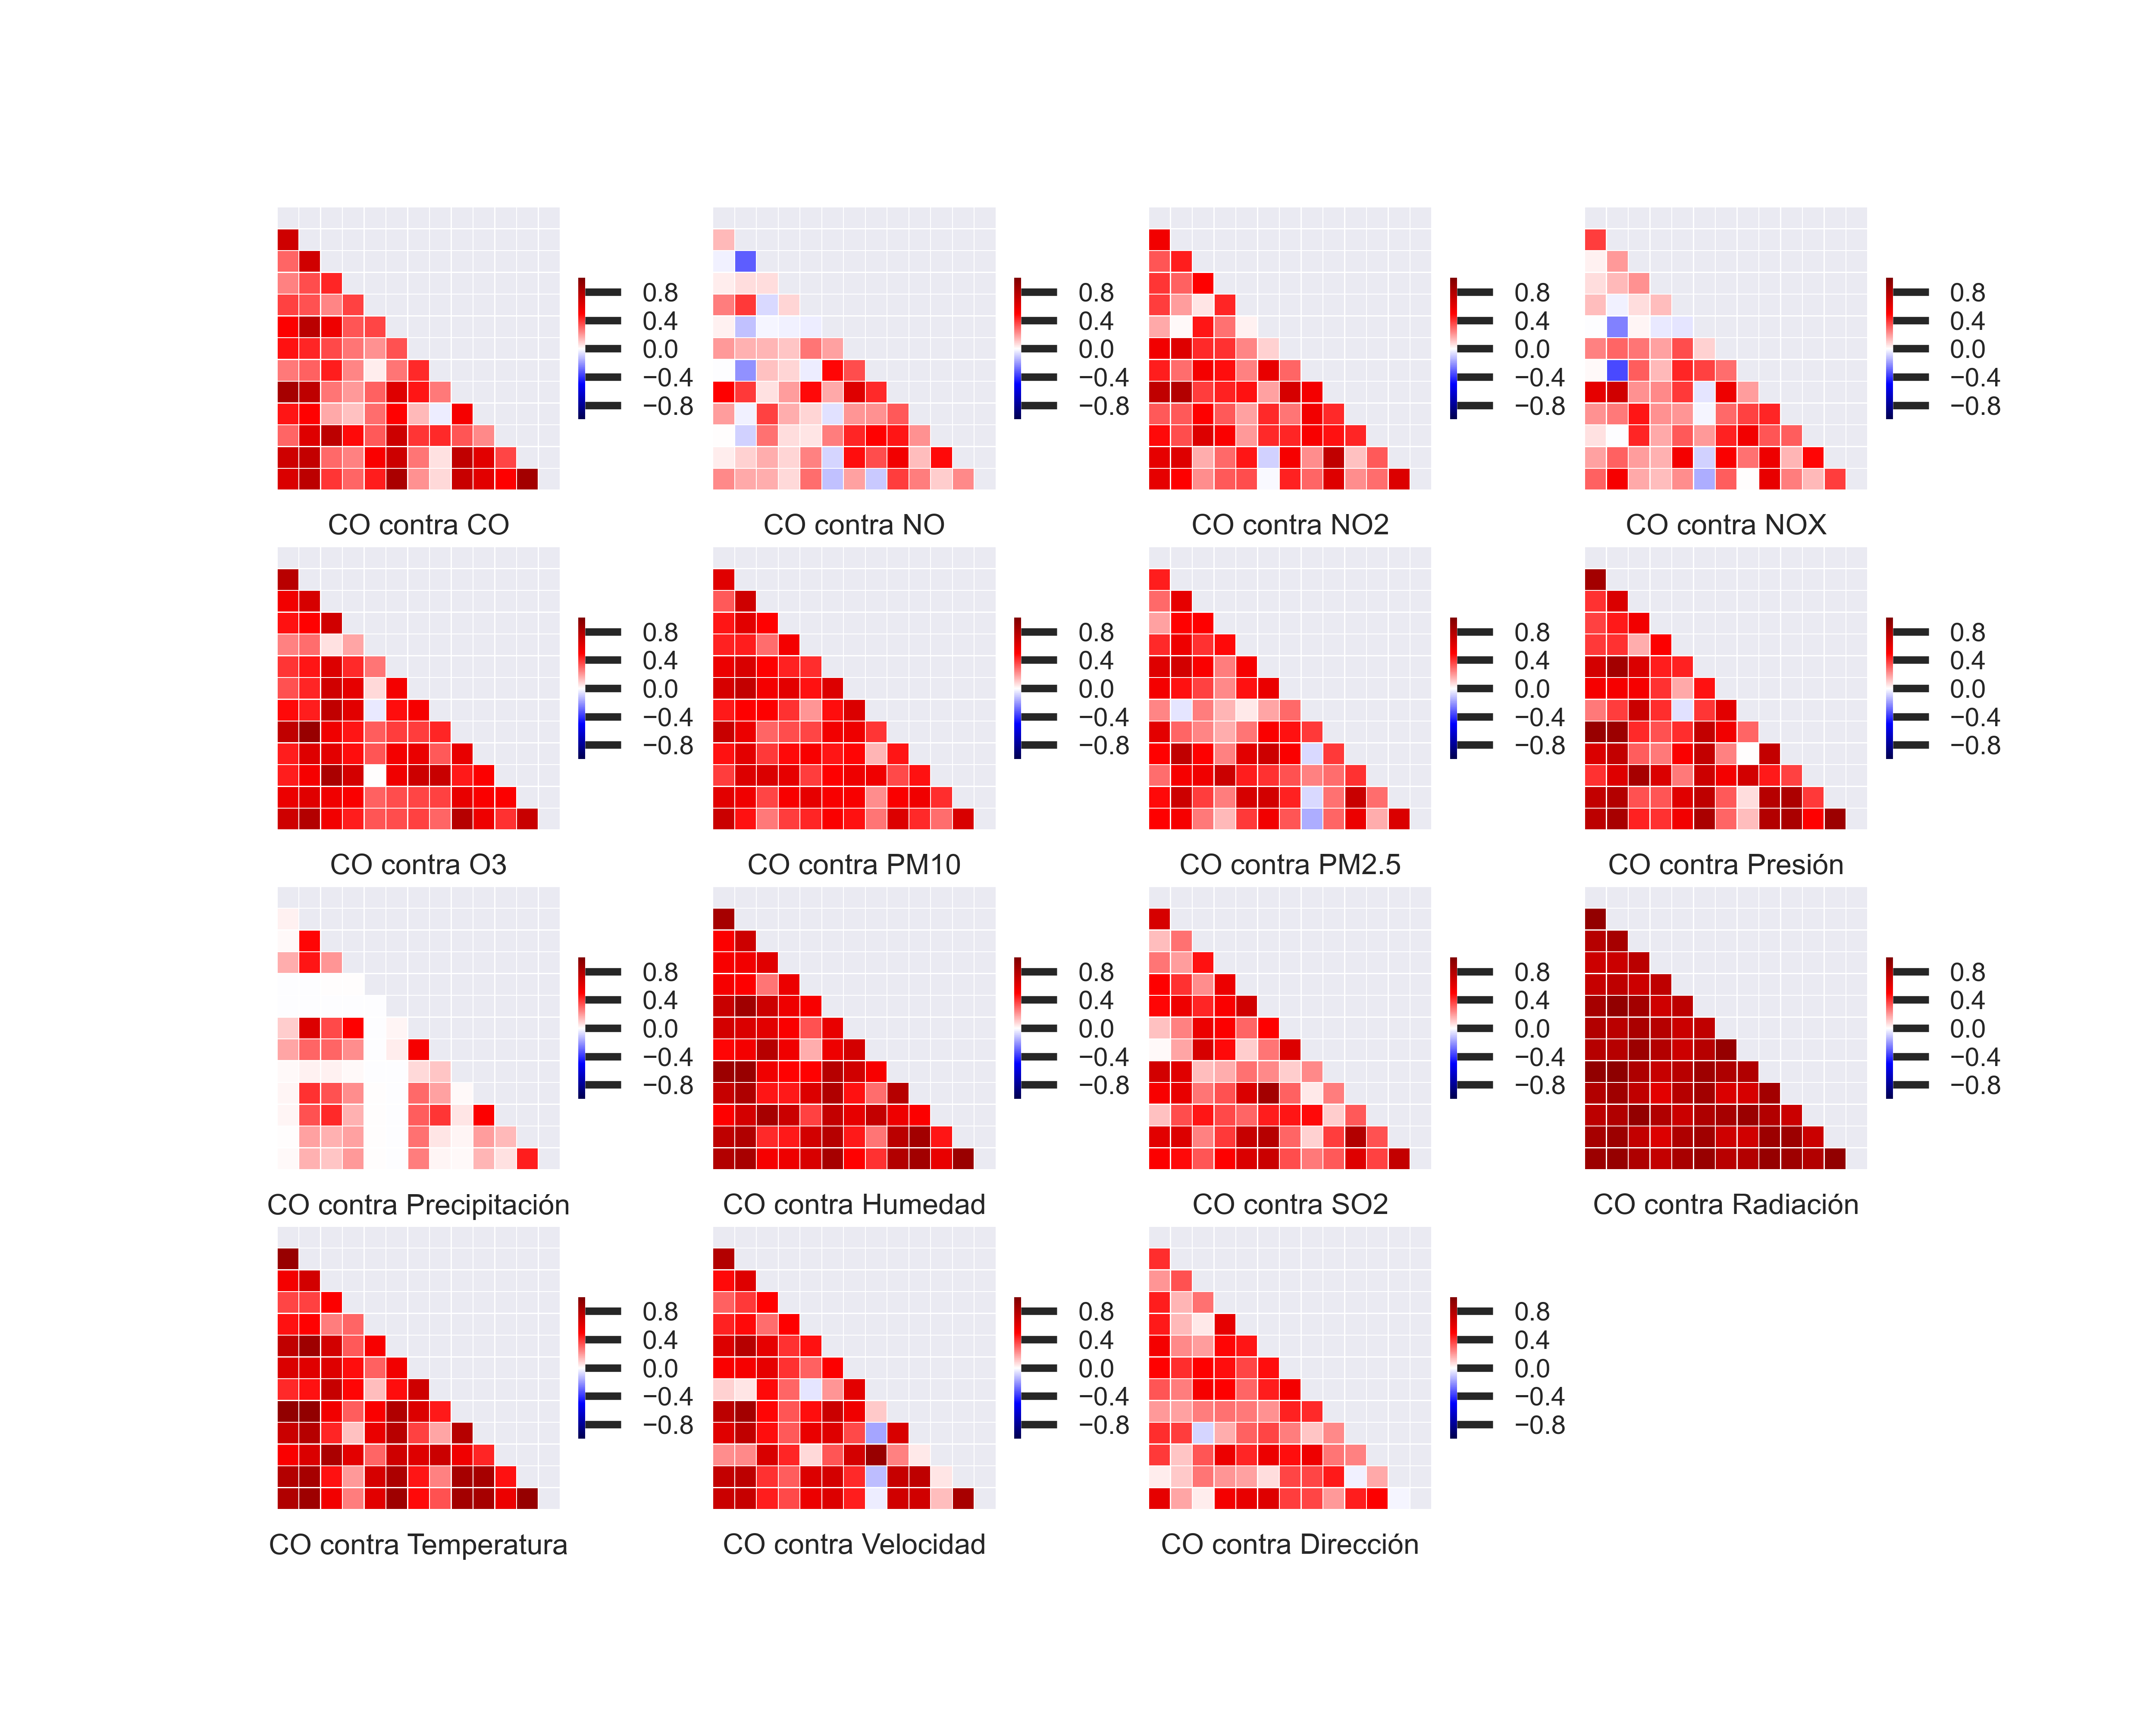
\includegraphics[width=15cm, height=13cm]{./Corr_CO_all_final}
\caption{Matriz de correlación de CO contra el resto de las variables}
\label{corrCO}
\end{figure}


La correlaciones de la variable CO con el resto de las variables se correlaciona positivamente mostrando correlaciones mayores a 0.2 (ver figura \ref{corrCO}), sin embargo para la variable {\em precipitación pluvial} las correlaciones son menores a 0.2 (ver figura \ref{corrCO}).






\subsection{Óxido Nítrico (NO)}
\begin{figure}[H]
\centering
\subfigure[Serie de tiempo de NO original] {\includegraphics[width=7cm, height=15cm]{./Serie_Nans_NO}}
\subfigure[Serie de tiempo de NO rellenando datos desconocidos]{\includegraphics[width=7cm, height=15cm]{./Serie_NO}}
\caption{Series de tiempo de NO desde 2016 hasta 2018}
\label{serieNO}
\end{figure}

La variable NO además de tener datos faltantes que se rellenan haciendo el promedio de las estaciones cercanas y asignando el promedio a las estaciones sin registros, se puede apreciar en la figura \ref{serieNO} que la serie de tiempo es estacionaria pues parece variar entorno a una media fija.

\begin{figure}[H]
\centering
\subfigure[Histograma de NO por estación] {\includegraphics[width=15cm, height=10cm]{./Histogram__3_NO_3}}
\subfigure[Histograma de NO]{\includegraphics[width=12cm, height=5cm]{./Histogram__3_NO_2}}
\caption{Histogramas de NO}
\label{histNO}
\end{figure}

La figura \ref{serieNO} muestra los gráficos de series de tiempo para la variable NO por estación y la figura \ref{histNO} muestra un histograma de los datos por estación de la variable NO. De la figura \ref{serieNO} se puede observar que si bien las trece series de tiempo muestran características muy similares, los histogramas de la figura \ref{histNO} son diferentes, ya que el histograma resume los datos a través de la dimensión del tiempo, y al hacerlo, se pierden las características clave de los datos que dependen del tiempo.

\begin{figure}[H]
\centering
\includegraphics[width=12cm, height=10cm]{./Corr_NO_NO}
\caption{Matriz de correlación de NO entre estaciones }
\label{corrNONO}
\end{figure}

La figura \ref{corrNONO} muestra que la variable NO se correlaciona positivamente alto (correlaciones mayores a 0.2) entre la mayoría de las estaciones, ya que las estaciones Centro y Sureste 2 muestran correlaciones menores a 0.2 contra el resto de la estaciones. Además para las estaciones Noroeste, Noreste y Norte muestran correlaciones bajas.

\begin{figure}[H]
\centering
\includegraphics[width=15cm, height=13cm]{./Corr_NO_all_final}
\caption{Matriz de correlación de NO contra el resto de las variables}
\label{corrNO}
\end{figure}


Para las correlaciones de la variable {\em precipitación pluvial} y NO$_{X}$, (ver figura \ref{corrNO}) se presentan en algunas estaciones correlaciones altas y correlaciones nulas. Además, para las correlaciones con la variable NO$_{2}$ presenta correlaciones positivas pequeñas para la estación Suroeste 2.





\subsection{Bióxido de Nitrógeno (NO$_{2}$)}
\begin{figure}[H]
\centering
\subfigure[Serie de tiempo de NO$_{2}$ original] {\includegraphics[width=7cm, height=15cm]{./Serie_Nans_NO2}}
\subfigure[Serie de tiempo de NO$_{2}$ rellenando datos desconocidos]{\includegraphics[width=7cm, height=15cm]{./Serie_NO2}}
\caption{Series de tiempo de NO$_{2}$ desde 2016 hasta 2018}
\label{serieNO2}
\end{figure}

La variable NO$_{2}$ presenta datos faltantes durante periodos de tiempo en los tres años que se rellenan haciendo el promedio de las estaciones cercanas, este promedio se le asigna a las estaciones sin registros. También, se puede apreciar en la figura \ref{serieNO2} (b), que la serie de tiempo es estacionaria, ya que parece variar entorno a una media, presentando altas variaciones en el mes de julio del 2017 en las trece estaciones.

\begin{figure}[H]
\centering
\subfigure[Histograma de NO$_{2}$ por estación] {\includegraphics[width=15cm, height=10cm]{./Histogram__4_NO2_3}}
\subfigure[Histograma de NO$_{2}$]{\includegraphics[width=12cm, height=5cm]{./Histogram__4_NO2_2}}
\caption{Histogramas de NO$_{2}$}
\label{histNO2}
\end{figure}

La figura \ref{serieNO2} muestra los gráficos de series de tiempo para la variable NO$_{2}$ por estación y la figura \ref{histNO2} muestra los histogramas de los datos por estación de la variable NO$_{2}$. En la figura \ref{serieNO2} se puede observar que si bien las trece series de tiempo muestran características muy similares, también,  los histogramas de la figura \ref{histNO2} son muy similares a excepción de las estaciones Norte 2 y Sur.

\begin{figure}[H]
\centering
\includegraphics[width=12cm, height=10cm]{./Corr_NO2_NO2}
\caption{Matriz de correlación de NO$_{2}$ entre estaciones }
\label{corrNO2NO2}
\end{figure}

La figura \ref{corrNO2NO2} muestra que la variable NO$_{2}$ se correlaciona positivamente entre la mayoria de las estaciones, ya que la estación Suroeste 2 muestra correlaciones bajas contra las estaciones Noroeste 2, Norte 2 y Suroeste.

\begin{figure}[H]
\centering
\includegraphics[width=15cm, height=13cm]{./Corr_NO2_all_final}
\caption{Matriz de correlación de NO$_{2}$ contra el resto de las variables}
\label{corrNO2}
\end{figure}

La estación Suroeste 2 presenta correlaciones positivas pequeñas contra la variable NO$_{X}$ (ver figura \ref{corrNO2}). Para las correlaciones de la variable {\em precipitación pluvial} se presentan en algunas estaciones correlaciones altas y correlaciones cercanas a cero (ver figura \ref{corrNO2}).






\subsection{Óxidos de Nitrógeno (NO$_{X}$)}
\begin{figure}[H]
\centering
\subfigure[Serie de tiempo de NO$_{X}$ original] {\includegraphics[width=7cm, height=15cm]{./Serie_Nans_NOX}}
\subfigure[Serie de tiempo de NO$_{X}$ rellenando datos desconocidos]{\includegraphics[width=7cm,height=15cm]{./Serie_NOX}}
\caption{Series de tiempo de NO$_{X}$ desde 2016 hasta 2018}
\label{serieNOX}
\end{figure}

La variable NO$_{X}$ además de tener datos faltantes que se rellenan haciendo el promedio de las estaciones cercanas y asignando el promedio a las estaciones sin registros, se puede apreciar en la figura \ref{serieNOX} que la serie de tiempo es estacionaria ya que parece variar en torno a una media fija.

\begin{figure}[H]
\centering
\subfigure[Histograma de NO$_{X}$ por estación] {\includegraphics[width=15cm, height=10cm]{./Histogram__5_NOX_3}}
\subfigure[Histograma de NO$_{X}$]{\includegraphics[width=12cm, height=5cm]{./Histogram__5_NOX_2}}
\caption{Histogramas de NO$_{X}$}
\label{histNOX}
\end{figure}

La figura \ref{serieNOX} muestra los gráficos de series de tiempo para la variable NO$_{X}$ por estación y la figura \ref{histNOX} muestra un histograma de los datos por estación de la variable NO$_{X}$. De la figura \ref{serieNOX} se puede apreciar que en las trece series de tiempo muestran características muy similares, sin embargo, los histogramas de la figura \ref{histNOX} son diferentes, ya que el histograma resume los datos a través de la dimensión del tiempo, y al hacer esto, se pierden las características importantes de los datos que dependen del tiempo.

\begin{figure}[H]
\centering
\includegraphics[width=12cm, height=10cm]{./Corr_NOX_NOX}
\caption{Matriz de correlación de NO$_{X}$ entre estaciones }
\label{corrNOXNOX}
\end{figure}

La correlación de la variable NO$_{X}$ entre estaciones (NO$_{X}$ vs NO$_{X}$) presenta correlaciones positivas pequeñas (ver figura \ref{corrNOXNOX}).  

\begin{figure}[H]
\centering
\includegraphics[width=15cm, height=13cm]{./Corr_NOX_all_final}
\caption{Matriz de correlación de NO$_{X}$  contra el resto de las variables}
\label{corrNOX}
\end{figure}

Las correlaciones de la variable {\em precipitación pluvial}  (ver Figura \ref{corrNOX}) muestran que para algunas correlaciones entre estaciones se presentan corelaciones positivas bajas.





\subsection{Ozono (O$_{3}$)}
\begin{figure}[H]
\centering
\subfigure[Serie de tiempo de O$_{3}$ original] {\includegraphics[width=7cm, height=15cm]{./Serie_Nans_O3}}
\subfigure[Serie de tiempo de O$_{3}$ rellenando datos desconocidos]{\includegraphics[width=7cm,height=15cm]{./Serie_O3}}
\caption{Series de tiempo de O$_{3}$ desde 2016 hasta 2018}
\label{serieO3}
\end{figure}

La variable O$_{3}$ además de tener datos faltantes que se completan haciendo el promedio de las estaciones cercanas y asignando el promedio a las estaciones sin registros, se puede apreciar en la figura \ref{serieO3} que la serie de tiempo es estacionaria pues varía entorno a un valor.

\begin{figure}[H]
\centering
\subfigure[Histograma de O$_{3}$ por estación] {\includegraphics[width=15cm, height=10cm]{./Histogram__6_O3_3}}
\subfigure[Histograma de O$_{3}$]{\includegraphics[width=12cm, height=5cm]{./Histogram__6_O3_2}}
\caption{Histogramas de O$_{3}$}
\label{histO3}
\end{figure}

La figura \ref{serieO3} muestra los gráficos de series de tiempo para la variable O$_{3}$ por estación y la figura \ref{histO3} muestra un histograma de los datos por estación de la variable O$_{3}$. De la figura \ref{serieO3} se puede observar que si bien las trece series de tiempo muestran características similares, los histogramas de la figura \ref{histO3} son distintos, pues el histograma resume los datos a través de la dimensión del tiempo, y al hacerlo, se pierden las características principales de los datos que dependen del tiempo.

\begin{figure}[H]
\centering
\includegraphics[width=12cm, height=10cm]{./Corr_O3_O3}
\caption{Matriz de correlación de O$_{3}$ entre estaciones }
\label{corrO32}
\end{figure}

La figura \ref{corrO32} muestra que la variable O$_{3}$ se correlaciona positivamente alto en todas las estaciones ya que la mayor correlación es de 0.99 entre las estaciones Noroeste 2 y Sur, mientras que la menor correlación encontrada es de 0.57 entre las estaciones Suroeste 2 y Sureste 2.

\begin{figure}[H]
\centering
\includegraphics[width=15cm, height=13cm]{./Corr_O3_all_final}
\caption{Matriz de correlación de O$_{3}$ contra el resto de las variables}
\label{corrO3}
\end{figure}

Para las correlaciones de la variable {\em precipitación pluvial} se presentan en algunas estaciones correlaciones altas y correlaciones cercanas a cero (ver figura \ref{corrO3}), para el resto de las variables la variable O$_{3}$ se correlaciona positivamente alto en todas las estaciones.





\subsection{Partículas Menores a 10 Micras (PM$_{10}$)}
\begin{figure}[H]
\centering
\subfigure[Serie de tiempo de PM$_{10}$ original] {\includegraphics[width=7cm, height=15cm]{./Serie_Nans_PM10}}
\subfigure[Serie de tiempo de PM$_{10}$ rellenando datos desconocidos]{\includegraphics[width=7cm,height=15cm]{./Serie_PM10}}
\caption{Series de tiempo de PM$_{10}$ desde 2016 hasta 2018}
\label{seriePM10}
\end{figure}

La variable PM$_{10}$ además de tener datos faltantes que se completan haciendo el promedio de las estaciones cercanas y luego se asigna el promedio a las estaciones sin datos, se puede apreciar en la figura \ref{seriePM10} que la serie de tiempo es estacionaria pues varía entorno a una media.

\begin{figure}[H]
\centering
\subfigure[Histograma de PM$_{10}$ por estación] {\includegraphics[width=15cm, height=10cm]{./Histogram__7_PM10_3}}
\subfigure[Histograma de PM$_{10}$]{\includegraphics[width=12cm, height=5cm]{./Histogram__7_PM10_2}}
\caption{Histogramas de PM$_{10}$}
\label{histPM10}
\end{figure}

La figura \ref{seriePM10} muestra los gráficos de series de tiempo para la variable PM$_{10}$ por estación y la figura \ref{histPM10} muestra un histograma de los datos por estación de la variable PM$_{10}$. De la figura \ref{seriePM10} se puede observar que las trece series de tiempo muestran características similares, pero, los histogramas de la figura \ref{histPM10} son diferentes, pues el histograma resume los datos a través de la dimensión del tiempo, y al hacer esto, se pierden las características principales de los datos que dependen del tiempo.

\begin{figure}[H]
\centering
\includegraphics[width=12cm, height=10cm]{./Corr_PM10_PM10}
\caption{Matriz de correlación de PM$_{10}$ entre estaciones }
\label{corrPM10_2}
\end{figure}

La figura \ref{corrPM10_2} muestra que la variable PM$_{10}$ se correlaciona positivamente alto entre todas las estaciones ya que la mayor correlación es de 0.73 entre las estaciones Norte 2 y Noreste, mientras que la menor correlación encontrada es de 0.20 entre las estaciones Noreste 2 y Noroeste 2.

\begin{figure}[H]
\centering
\includegraphics[width=15cm, height=13cm]{./Corr_PM10_all_final}
\caption{Matriz de correlación de PM$_{10}$ contra el resto de las variables}
\label{corrPM10}
\end{figure}


Para las correlaciones de la variable {\em precipitación pluvial} se presentan algunas estaciones con correlaciones altas y correlaciones cercanas a cero (ver figura \ref{corrPM10}), para el resto de las variables la variable PM$_{10}$ se correlaciona positivamente alto en todas las estaciones.





\subsection{Partículas Menores a 2.5 Micras (PM$_{2.5}$)}
\begin{figure}[H]
\centering
\subfigure[Serie de tiempo de PM$_{2.5}$ original] {\includegraphics[width=7cm, height=15cm]{./Serie_Nans_PM2_5}}
\subfigure[Serie de tiempo de PM$_{2.5}$ rellenando datos desconocidos]{\includegraphics[width=7cm,height=15cm]{./Serie_PM2_5}}
\caption{Series de tiempo de PM$_{2.5}$ desde 2016 hasta 2018}
\label{seriePM2_5}
\end{figure}

La variable PM$_{2.5}$ además de tener datos faltantes que se rellenan haciendo el promedio de las estaciones cercanas y asignando el promedio a las estaciones sin registros, se puede apreciar en la figura \ref{seriePM2_5} que la serie de tiempo es estacionaria ya que parece variar en torno a una media fija.

\begin{figure}[H]
\centering
\subfigure[Histograma de PM$_{2.5}$ por estación] {\includegraphics[width=15cm, height=10cm]{./Histogram__8_PM2_5_3}}
\subfigure[Histograma de PM$_{2.5}$]{\includegraphics[width=12cm, height=5cm]{./Histogram__8_PM2_5_2}}
\caption{Histogramas de PM$_{2.5}$}
\label{histPM2_5}
\end{figure}

La figura \ref{seriePM2_5} muestra los gráficos de series de tiempo para la variable PM$_{2.5}$ por estación y la figura \ref{histPM2_5} muestra un histograma de los datos por estación de la variable PM$_{2.5}$. De la figura \ref{seriePM2_5} se puede observar que si bien las trece series de tiempo muestran características muy similares, los histogramas de la figura \ref{histPM2_5} son diferentes, ya que el histograma resume los datos a través de la dimensión del tiempo, y al hacerlo, se pierden las características clave de los datos que dependen del tiempo.

\begin{figure}[H]
\centering
\includegraphics[width=12cm, height=10cm]{./Corr_PM2_5_PM2_5}
\caption{Matriz de correlación de PM$_{2.5}$ entre estaciones }
\label{corrPM25_2}
\end{figure}

La figura \ref{corrPM25_2} muestra que la variable PM$_{2.5}$ se correlaciona positivamente alto entre todas las estaciones ya que la mayor correlación es de 0.97 entre las estaciones Norte y Sur, mientras que la menor correlación encontrada es de 0.28 entre las estaciones Sur y Noroeste.

\begin{figure}[H]
\centering
\includegraphics[width=15cm, height=13cm]{./Corr_PM2_5_all_final}
\caption{Matriz de correlación de PM$_{2.5}$ contra el resto de las variables}
\label{corrPM2_5}
\end{figure}


Para las correlaciones de la variable {\em precipitación pluvial} se presentan en algunas estaciones correlaciones altas y correlaciones cercanas a cero (ver figura \ref{corrPM2_5}), para el resto de las variables la variable PM$_{2.5}$ se correlaciona positivamente alto en todas las estaciones.




\subsection{Presión Barométrica}
\begin{figure}[H]
\centering
\subfigure[Serie de tiempo de {\em presión barométrica} original] {\includegraphics[width=7cm, height=15cm]{./Serie_Nans_pressure}}
\subfigure[Serie de tiempo de {\em presión barométrica} rellenando datos desconocidos]{\includegraphics[width=7cm,height=15cm]{./Serie_pressure}}
\caption{Series de tiempo de {\em presión barométrica} desde 2016 hasta 2018}
\label{seriePressure}
\end{figure}

La variable {\em presión barométrica} además de tener datos faltantes que se rellenan haciendo el promedio de las estaciones cercanas y asignando el promedio a las estaciones sin registros, se puede apreciar en la figura \ref{seriePressure} que la serie de tiempo es estacionaria ya que parece variar entorno a una media.

\begin{figure}[H]
\centering
\subfigure[Histograma de {\em presión barométrica} por estación] {\includegraphics[width=15cm, height=10cm]{./Histogram__9_Pressure_3}}
\subfigure[Histograma de {\em presión barométrica}]{\includegraphics[width=12cm, height=5cm]{./Histogram__9_Pressure_2}}
\caption{Histogramas de {\em presión barométrica}}
\label{histPressure}
\end{figure}

La figura \ref{seriePressure} muestra los gráficos de series de tiempo para la variable {\em presión barométrica} por estación y la figura \ref{histPressure} muestra un histograma de los datos por estación de la variable {\em presión barométrica}. De la figura \ref{seriePressure} se puede observar que si bien las trece series de tiempo muestran características muy similares, los histogramas de la figura \ref{histPressure} son diferentes, ya que el histograma resume los datos a través de la dimensión del tiempo, y al hacerlo, se pierden las características más importantes de los datos que dependen del tiempo.

\begin{figure}[H]
\centering
\includegraphics[width=12cm, height=10cm]{./Corr_pressure_pressure}
\caption{Matriz de correlación de {\em presión barométrica} entre estaciones }
\label{corrpressure2}
\end{figure}

La figura \ref{corrpressure2} muestra que la variable {\em presión barométrica} se correlaciona positivamente alto entre la mayoría de las estaciones ya que la estación Sureste 3 presenta dos correlaciones positivas bajas contra las estaciones Noroeste 2 y Sureste y una correlación negativa alta contra la estación Sur.

\begin{figure}[H]
\centering
\includegraphics[width=15cm, height=13cm]{./Corr_PM2_5_all_final}
\caption{Matriz de correlación de {\em presión  barométrica} contra el resto de las variables}
\label{corrpressure}
\end{figure}

Para las correlaciones de la variable {\em precipitación pluvial} se presentan en algunas estaciones correlaciones altas y correlaciones cercanas a cero (ver figura \ref{corrpressure}), para el resto de las variables la variable O$_{3}$ se correlaciona positivamente alto en todas las estaciones.





\subsection{Precipitación Pluvial}
\begin{figure}[H]
\centering
\subfigure[Serie de tiempo de {\em precipitación pluvial} original] {\includegraphics[width=7cm, height=15cm]{./Serie_Nans_rainfall}}
\subfigure[Serie de tiempo de {\em precipitación pluvial} rellenando datos desconocidos]{\includegraphics[width=7cm,height=15cm]{./Serie_rainfall}}
\caption{Series de tiempo de {\em precipitación pluvial} desde 2016 hasta 2018}
\label{serierainfall}
\end{figure}

La variable {\em precipitación pluvial} además de tener datos faltantes que se rellenan haciendo el promedio de las estaciones cercanas y asignando el promedio a las estaciones sin registros, se puede apreciar en la figura \ref{serierainfall} que la serie de tiempo es estacionaria ya que parece variar en torno a una media fija.

\begin{figure}[H]
\centering
\subfigure[Histograma de {\em precipitación pluvial} por estación] {\includegraphics[width=15cm, height=10cm]{./Histogram__10_rainfall_3}}
\subfigure[Histograma de {\em precipitación pluvial}]{\includegraphics[width=12cm, height=5cm]{./Histogram__10_rainfall_2}}
\caption{Histogramas de {\em precipitación pluvial} }
\label{histPressure}
\end{figure}

La figura \ref{seriePressure} muestra los gráficos de series de tiempo para la variable {\em precipitación pluvial} por estación y la figura \ref{histPressure} muestra un histograma de los datos por estación de la variable {\em precipitación pluvial}. De la figura \ref{seriePressure} se puede observar que si bien las trece series de tiempo muestran características muy similares, los histogramas de la figura \ref{histPressure} son diferentes, ya que el histograma resume los datos a través de la dimensión del tiempo, y al hacerlo, se pierden las características clave de los datos que dependen del tiempo.

\begin{figure}[H]
\centering
\includegraphics[width=12cm, height=10cm]{./Corr_rainfall_rainfall}
\caption{Matriz de correlación de {\em precipitación pluvial} entre estaciones }
\label{corrrainfall2}
\end{figure}

La figura \ref{corrrainfall2} muestra que la variable {\em precipitación pluvial} no se correlaciona con ninguna de las variables restantes.

\begin{figure}[H]
\centering
\includegraphics[width=15cm, height=13cm]{./Corr_rainfall_all_final}
\caption{Matriz de correlación de {\em precipitación pluvial} contra el resto de las variables}
\label{corrrainfall}
\end{figure}


Para las correlaciones de la variable {\em precipitación pluvial} con el resto de las variables presentan en algunas estaciones correlaciones altas y correlaciones cercanas a cero (ver figura \ref{corrrainfall}), es decir, aunque esta variable no se correlaciona con el resto de las variables, en las pocas en las que si lo hace, sucede de manera positiva.




\subsection{Humedad Relativa}
\begin{figure}[H]
\centering
\subfigure[Serie de tiempo de {\em humedad relativa} original] {\includegraphics[width=7cm, height=15cm]{./Serie_Nans_humidity}}
\subfigure[Serie de tiempo de {\em humedad relativa} rellenando datos desconocidos]{\includegraphics[width=7cm,height=15cm]{./Serie_humidity}}
\caption{Series de tiempo de {\em humedad relativa} desde 2016 hasta 2018}
\label{seriehumidity}
\end{figure}

La variable {\em humedad relativa} además de tener datos faltantes que se rellenan haciendo el promedio de las estaciones cercanas y asignando el promedio a las estaciones sin registros, se puede apreciar en la figura \ref{seriehumidity} que la serie de tiempo es estacionaria ya que parece variar entorno a un valor fijo.

\begin{figure}[H]
\centering
\subfigure[Histograma de {\em humedad relativa} por estación] {\includegraphics[width=15cm, height=10cm]{./Histogram__11_humidity_3}}
\subfigure[Histograma de {\em humedad relativa}]{\includegraphics[width=12cm, height=5cm]{./Histogram__11_humidity_2}}
\caption{Histogramas de {\em humedad relativa} }
\label{histhumidity}
\end{figure}

La figura \ref{seriehumidity} muestra los gráficos de series de tiempo para la variable {\em humedad relativa} por estación y la figura \ref{histhumidity} muestra un histograma de los datos por estación de la variable {\em humedad relativa}. De la figura \ref{seriehumidity} se puede observar que si bien las trece series de tiempo muestran características muy similares, los histogramas de la figura \ref{histhumidity} son diferentes, ya que el histograma resume los datos a través de la dimensión del tiempo, y al hacerlo, se pierden las características clave de los datos que dependen del tiempo.

\begin{figure}[H]
\centering
\includegraphics[width=12cm, height=10cm]{./Corr_humidity_humidity}
\caption{Matriz de correlación de {\em humedad relativa} entre estaciones }
\label{corrhumidity2}
\end{figure}

La figura \ref{corrhumidity2} muestra que la variable {\em humedad relativa} se correlaciona positivamente alto entrel a mayoría de las estaciones ya que la estación Norte presenta dos correlaciones positivas bajas contra el resto de las demás estaciones.

\begin{figure}[H]
\centering
\includegraphics[width=15cm, height=13cm]{./Corr_humidity_all_final}
\caption{Matriz de correlación de {\em humedad relativa} contra el resto de las variables}
\label{corrhumidity}
\end{figure}

La variable {\em humedad relativa} se correlaciona con el resto de las variables positivamente alto en todas las variables restantes (ver figura \ref{corrhumidity}).




\subsection{Bióxido de Azufre (SO$_{2}$)}
\begin{figure}[H]
\centering
\subfigure[Serie de tiempo de SO$_{2}$ original] {\includegraphics[width=7cm, height=15cm]{./Serie_Nans_SO2}}
\subfigure[Serie de tiempo de SO$_{2}$ rellenando datos desconocidos]{\includegraphics[width=7cm,height=15cm]{./Serie_SO2}}
\caption{Series de tiempo de SO$_{2}$ desde 2016 hasta 2018}
\label{serieSO2}
\end{figure}

La variable SO$_{2}$ además de tener datos faltantes que se completan haciendo el promedio de las estaciones cercanas y asignando el promedio a las estaciones sin registros, se puede apreciar en la figura \ref{serieSO2} que la serie de tiempo es estacionaria ya que parece variar en torno a un valor.

\begin{figure}[H]
\centering
\subfigure[Histograma de SO$_{2}$ por estación] {\includegraphics[width=15cm, height=10cm]{./Histogram__12_SO2_3}}
\subfigure[Histograma de SO$_{2}$]{\includegraphics[width=12cm, height=5cm]{./Histogram__12_SO2_2}}
\caption{Histogramas de SO$_{2}$}
\label{histSO2}
\end{figure}

La figura \ref{serieSO2} muestra los gráficos de series de tiempo para la variable SO$_{2}$ por estación y la figura \ref{histSO2} muestra un histograma de los datos por estación de la variable SO$_{2}$. De la figura \ref{serieSO2} se puede observar que si bien las trece series de tiempo muestran características muy similares, los histogramas de la figura \ref{histSO2} son diferentes, ya que el histograma resume los datos a través de la dimensión del tiempo, y al hacerlo, se pierden las características clave de los datos que dependen del tiempo.

\begin{figure}[H]
\centering
\includegraphics[width=12cm, height=10cm]{./Corr_SO2_SO2}
\caption{Matriz de correlación de SO$_{2}$ entre estaciones }
\label{corrSO2_2}
\end{figure}

La figura \ref{corrSO2_2} muestra que la variable SO$_{2}$ casi no se correlaciona entre estaciones ya que la mayoría de las correlaciones entre estaciones son muy cercanas a cero, mientras que el resto de las estaciones se correlacionan de manera positiva.

\begin{figure}[H]
\centering
\includegraphics[width=15cm, height=13cm]{./Corr_SO2_all_final}
\caption{Matriz de correlación SO$_{2}$ contra el resto de las variables}
\label{corrSO2}
\end{figure}


Para las correlaciones de la variable {\em dirección del viento} se presentan en algunas estaciones correlaciones positivas pequeñas (ver figura \ref{corrSO2}). Para el resto de las variables, la variable SO$_{2}$ se correlaciona positivamente alto en todas las estaciones.



\subsection{Radiación Solar}
\begin{figure}[H]
\centering
\subfigure[Serie de tiempo de {\em radiación solar} original] {\includegraphics[width=7cm, height=15cm]{./Serie_Nans_solar}}
\subfigure[Serie de tiempo de {\em radiación solar} rellenando datos desconocidos]{\includegraphics[width=7cm,height=15cm]{./Serie_solar}}
\caption{Series de tiempo de {\em radiación solar} desde 2016 hasta 2018}
\label{seriesolar}
\end{figure}

La variable {\em radiación solar} además de tener datos faltantes que se rellenan haciendo el promedio de las estaciones cercanas y asignando el promedio a las estaciones sin registros, se puede apreciar en la figura \ref{seriesolar} que la serie de tiempo es estacionaria ya que parece variar en torno a una media fija.

\begin{figure}[H]
\centering
\subfigure[Histograma de {\em radiación solar por estación}] {\includegraphics[width=15cm, height=10cm]{./Histogram__13_solar_3}}
\subfigure[Histograma de {\em radiación solar}]{\includegraphics[width=12cm, height=5cm]{./Histogram__13_solar_2}}
\caption{Histogramas de {\em radiación solar}}
\label{histsolar}
\end{figure}

La figura \ref{seriesolar} muestra los gráficos de series de tiempo para la variable {\em radiación solar} por estación y la figura \ref{histsolar} muestra un histograma de los datos por estación de la variable {\em radiación solar}. De la figura \ref{seriesolar} se puede observar que si bien las trece series de tiempo muestran características muy similares, los histogramas de la figura \ref{histsolar} son diferentes, ya que el histograma resume los datos a través de la dimensión del tiempo, y al hacerlo, se pierden las características clave de los datos que dependen del tiempo.

\begin{figure}[H]
\centering
\includegraphics[width=12cm, height=10cm]{./Corr_solar_solar}
\caption{Matriz de correlación de {\em radiación solar} entre estaciones }
\label{corrsolar2}
\end{figure}

La figura \ref{corrsolar2} muestra que la variable {\em radiación solar} se correlaciona positivamente alto entre todas las estaciones.

\begin{figure}[H]
\centering
\includegraphics[width=15cm, height=13cm]{./Corr_solar_all_final}
\caption{Matriz de correlación de {\em radiación solar} contra el resto de las variables}
\label{corrsolar}
\end{figure}

Para las correlaciones de la variable {\em radiación solar} se presentan correlaciones positivas altas para todas las estaciones en todas cuando se hace contra el resto de variables restantes (ver figura \ref{corrsolar}). 




\subsection{Temperatura Ambiental}
\begin{figure}[H]
\centering
\subfigure[Serie de tiempo de {\em temperatura ambiental} original] {\includegraphics[width=7cm, height=15cm]{./Serie_Nans_temperature}}
\subfigure[Serie de tiempo de {\em temperatura ambiental} rellenando datos desconocidos]{\includegraphics[width=7cm,height=15cm]{./Serie_temperature}}
\caption{Series de tiempo de {\em temperatura ambiental} desde 2016 hasta 2018}
\label{serietemperature}
\end{figure}

La variable {\em temperatura ambiental} además de tener datos faltantes que se rellenan haciendo el promedio de las estaciones cercanas y asignando el promedio a las estaciones sin registros, se puede apreciar en la figura \ref{serietemperature} que la serie de tiempo es estacionaria ya que parece variar en torno a una media fija.

\begin{figure}[H]
\centering
\subfigure[Histograma de {\em temperatura ambiental} por estación] {\includegraphics[width=15cm, height=10cm]{./Histogram__14_temperature_3}}
\subfigure[Histograma de {\em temperatura ambiental}]{\includegraphics[width=12cm, height=5cm]{./Histogram__14_temperature_2}}
\caption{Histogramas de {\em temperatura ambiental}}
\label{histtemperature}
\end{figure}

La figura \ref{serietemperature} muestra los gráficos de series de tiempo para la variable {\em temperatura ambiental} por estación y la figura \ref{histtemperature} muestra un histograma de los datos por estación de la variable {\em temperatura ambiental}. De la figura \ref{serietemperature} se puede observar que si bien las trece series de tiempo muestran características muy similares, los histogramas de la figura \ref{histtemperature} son diferentes, ya que el histograma resume los datos a través de la dimensión del tiempo, y al hacerlo, se pierden las características clave de los datos que dependen del tiempo.

\begin{figure}[H]
\centering
\includegraphics[width=12cm, height=10cm]{./Corr_temperature_temperature}
\caption{Matriz de correlación de {\em temperatura ambiental} entre estaciones }
\label{corrtemperature2}
\end{figure}

La figura \ref{corrtemperature2} muestra que la variable {\em temperatura ambiental} se correlaciona positivamente alto entre todas las estaciones.

\begin{figure}[H]
\centering
\includegraphics[width=15cm, height=13cm]{./Corr_temperature_all_final}
\caption{Matriz de correlación de {\em temperatura ambiental} contra el resto de las variables}
\label{corrtemperature}
\end{figure}

Para las correlaciones de la variable {\em temperatura ambiental} se presentan correlaciones positivas altas para todas las estaciones en todas cuando se hace contra el resto de variables restantes (ver figura \ref{corrtemperature}). 





\subsection{Velocidad del Viento}
\begin{figure}[H]
\centering
\subfigure[Serie de tiempo de {\em velocidad del viento} original] {\includegraphics[width=7cm, height=15cm]{./Serie_Nans_velocity}}
\subfigure[Serie de tiempo de {\em velocidad del viento} rellenando datos desconocidos]{\includegraphics[width=7cm,height=15cm]{./Serie_velocity}}
\caption{Series de tiempo de {\em velocidad del viento} desde 2016 hasta 2018}
\label{serievelocity}
\end{figure}

La variable {\em velocidad del viento} además de tener datos faltantes que se rellenan haciendo el promedio de las estaciones cercanas y asignando el promedio a las estaciones sin registros, se puede apreciar en la figura \ref{serievelocity} que la serie de tiempo es estacionaria ya que parece variar en torno a un valor constante.

\begin{figure}[H]
\centering
\subfigure[Histograma de {\em velocidad del viento} por estación] {\includegraphics[width=15cm, height=10cm]{./Histogram__15_velocity_3}}
\subfigure[Histograma de {\em velocidad del viento}]{\includegraphics[width=12cm, height=5cm]{./Histogram__15_velocity_2}}
\caption{Histogramas de {\em velocidad del viento}}
\label{histvelocity}
\end{figure}

La figura \ref{serievelocity} muestra los gráficos de series de tiempo para la variable {\em velocidad del viento} por estación y la figura \ref{histvelocity} muestra un histograma de los datos por estación de la variable {\em velocidad del viento}. De la figura \ref{serievelocity} se puede observar que si bien las trece series de tiempo muestran características muy similares, los histogramas de la figura \ref{histvelocity} son diferentes, ya que el histograma resume los datos a través de la dimensión del tiempo, y al hacerlo, se pierden las características principales de los datos que dependen del tiempo.

\begin{figure}[H]
\centering
\includegraphics[width=12cm, height=10cm]{./Corr_velocity_velocity}
\caption{Matriz de correlación de {\em velocidad del viento} entre estaciones }
\label{corrvelocity2}
\end{figure}

La figura \ref{corrvelocity2} muestra que la variable {\em velocidad del viento} se correlaciona positivamente alto entre todas las estaciones, menos en la estación Centro ya que presenta correlaciones menores a 0.2 entre la mayoria de las estaciones 

\begin{figure}[H]
\centering
\includegraphics[width=15cm, height=13cm]{./Corr_temperature_all_final}
\caption{Matriz de correlación de {\em velocidad del viento} contra el resto de las variables}
\label{corrvelocity}
\end{figure}


Para las correlaciones de la variable {\em velocidad del viento} se presentan correlaciones positivas altas para todas las estaciones en todas cuando se hace contra el resto de variables restantes (ver figura \ref{corrvelocity}).





\subsection{Dirección del Viento}
\begin{figure}[H]
\centering
\subfigure[Serie de tiempo de {\em dirección del viento} original] {\includegraphics[width=7cm, height=15cm]{./Serie_Nans_direction}}
\subfigure[Serie de tiempo de {\em dirección del viento} rellenando datos desconocidos]{\includegraphics[width=7cm,height=15cm]{./Serie_direction}}
\caption{Series de tiempo de {\em dirección del viento} desde 2016 hasta 2018}
\label{seriedirection}
\end{figure}

La variable {\em dirección del viento} además de tener datos faltantes que se rellenan haciendo el promedio de las estaciones cercanas y asignando el promedio a las estaciones sin registros, se puede apreciar en la figura \ref{seriedirection} que la serie de tiempo es estacionaria ya que parece variar en torno a una media.

\begin{figure}[H]
\centering
\subfigure[Histograma de {\em dirección del viento} por estación] {\includegraphics[width=15cm, height=10cm]{./Histogram__16_direction_3}}
\subfigure[Histograma de {\em dirección del viento}]{\includegraphics[width=12cm, height=5cm]{./Histogram__16_direction_2}}
\caption{Histogramas de {\em dirección del viento}}
\label{histdirection}
\end{figure}

La figura \ref{seriedirection} muestra los gráficos de series de tiempo para la variable {\em dirección del viento} por estación y la figura \ref{histdirection} muestra un histograma de los datos por estación de la variable {\em dirección del viento}. De la figura \ref{seriedirection} se puede observar que si bien las trece series de tiempo muestran características muy similares, los histogramas de la figura \ref{histdirection} son diferentes, ya que el histograma resume los datos a través de la dimensión del tiempo, y al hacerlo, se pierden las características clave de los datos que dependen del tiempo.

\begin{figure}[H]
\centering
\includegraphics[width=12cm, height=10cm]{./Corr_direction_direction}
\caption{Matriz de correlación de {\em dirección del viento} entre estaciones }
\label{corrdirection}
\end{figure}

Para las correlaciones de la variable {\em dirección del viento} se presentan correlaciones positivas altas (ver figura \ref{corrdirection}).

\begin{figure}[H]
\centering
\includegraphics[width=15cm, height=13cm]{./Corr_direction_all_final}
\caption{Matriz de correlación de {\em dirección del viento} contra el resto de las variables}
\label{corrdirection}
\end{figure}






\section{Medición del Error}

A partir de una {\em validación cruzada} (eliminar una o varias estaciones para interpolar su valor con base en la información restante) y se comparan los valores reales e interpolados a partir de los métodos: 

\begin{itemize}
\item Error porcentual absoluto medio
\[ \text{MAPE} = \frac{1}{T} \sum_{t=1}^{T} \frac{|\hat{y}_{x_{i},t} -y_{x_{i},t}|}{y_{x_{i},t}}. \]
\item Error absoluto medio
\[ \text{MAE} = \frac{1}{T} \sum_{t=1}^{T} |\hat{y}_{x_{i},t}-y_{x_{i},t}|. \]
\item Error cuadrático medio
\[ \text{MSE} = \frac{1}{T} \sum_{t=1}^{T} (\hat{y}_{x_{i},t}-y_{x_{i},t})^{2}. \]
\item Error cuadrático medio 
\[ \text{RMSE} = \sqrt{ \frac{1}{T} \sum_{t=1}^{T} (\hat{y}_{x_{i},t}-y_{x_{i},t})^{2}}, \]
\end{itemize}

donde $y_{x_{i},t}$ es el valor real en la estación $x_{i}$ al tiempo $t$, $\hat{y}_{x_{i},t}$ es el valor predicho en la estación $x_{i}$ al tiempo $t$ y $T$ es el número total de iteraciones.

\subsection{Error}
Se define el {\em error} entre un pronóstico contra el valor real observado como:
\[ e_{t} = \hat{y}_{x_{i},t} -y_{x_{i},t}, \]
donde $y_{x_{i},t}$ es el valor real en la estación $x_{i}$ al tiempo $t$, $\hat{y}_{x_{i},t}$ es el valor predicho en la estación $x_{i}$ al tiempo $t$.

Con esta definición, si el pronóstico supera el valor real, el error será positivo y si el pronóstico no supera la demanda el error será negativo. 

\subsection{MAPE}
El {\em error porcentual absoluto medio} (MAPE) es una medida de error que se encuentra entre los más utilizados para medir la presición del pronóstico.

La idea de MAPE consiste en la suma de los errores absolutos individuales divididos por el valor real (en cada período por separado) o el promedio de los errores porcentuales.  Un problema que se puede ver de esta métrica, es que MAPE divide cada error individual por el valor real, por lo que está sesgado, es decir, los errores altos durante los periodos de valores reales pequeños tendrán un gran impacto en el valor de MAPE, además de presentarse el caso en el que el valor real observado sea cero, el MAPE producirá errores al ser evaluado.

\subsection{MAE}
El {\em error absoluto medio} (MAE) es uno de las métricas también más utilizadas para medir la precisión del pronóstico. La idea de MAE es hacer la media del error absoluto.

Un problema que presenta esta métrica es que no se ajusta a los valores reales promedio, por ejemplo si al calcular MAE el resultado es diez, no se sabe si esto es bueno o malo, es decir, si sus valores reales promedio es de mil, el MAE es muy bueno, pero si los errores reales promedio son uno, la precisión en este caso es mala. Para tratar con este problema se suele dividir MAE entre los valores reales promedio para obtener un porcentaje de la siguiente manera: \[ \text{MAEP} = \frac{\text{MAE}}{\frac{1}{n}\sum_{t=0}^{n} y_{x_{i},t}}, \]
al cual se llamará para este trabajo de tesis {\em error absoluto medio porcentual} (MAEP).
\subsection{RMSE}
El {\em error cuadrático medio} (RMSE) es una métrica que se define como la raíz cuadrada del error cuadrado promedio, entonces RMSE al igual que MAE no se adapta al promedio de los valores reales. Para tratar con este problema se suele hacer:
\[\text{RMSEP} = \frac{\text{RMSE}}{\frac{1}{n}\sum_{t=0}^{n} y_{x_{i},t}}, \]
al cual se llamará {\em error cuadrático medio porcentual} (RMSEP). A diferencia del MAE, el RMSE no trata cada error de la misma manera, es decir, da más importancia a los errores más grandes. Eso implica que un gran error basta para obtener un mal RMSE.

\subsection{MSE}
El {\em error cuadrático medio} (MSE) es utilizado por muchos algoritmos ya que es más rápido y fácil de calcular que otras métricas, pero al estar el error al cuadrado, MSE no se ajusta al valor del error original, lo que resulta en una métrica que no se puede relacionar directamente entre la predicción y el valor real observado.

En conclusión MAE brinda protección contra los valores atípicos, mientras que RMSE brinda la seguridad de obtener un pronóstico imparcial. Si se usa MAE como métrica de error dará como resultado un alto sesgo, por lo que es probable que se escoja usar RMSE. Por otro lado, si el conjunto de datos contiene muchos valores atípicos, resultará en un pronóstico sesgado, por lo que es posible que se utilice la métrica MAE.

Para este trabajo de tesis se evalúan las siguientes métricas mencionadas en el orden siguiente:
\begin{enumerate}
\item MAPE
\item MAE
\item MAEP
\item RMSE
\item RMSEP
\item MSE
\end{enumerate}



\section{Entorno Computacional y Tiempo de Ejecución}
Para la parte de programación de este trabajo de tesis se utiliza para ejecutar el código correspondiente \citep{sernagit}, una  computadora con sistema operativo Windows 10 Home de 64 bits, procesador Intel \texttt{Core i-7 2.2 GHz} y 8 GB de RAM. Lenguaje de programación \texttt{Python versión 3.7.}

\begin{figure}[H]
\centering
\includegraphics[width=13cm, height=13cm]{./Time}
\caption{Tiempos de ejecución}
\label{time}
\end{figure}

En la figura \ref{time} se muestran los tiempos de ejecución para los cuatro escenarios: nueve, diez, once y doce estaciones seleccionadas para interpolar: cuatro, tres, dos y una estación respectivamente. Se puede ver que los tiempos de ejecución decrecen conforme se aumenta el número de estaciones seleccionas. Primero, se ve que el tiempo de ejecución de la interpolación aumenta muy poco conforme aumenta la cantidad de estaciones seleccionadas, de cinco horas con 21 minutos a cinco horas con 22 minutos. Después, se observa en los tiempos de ejecución de la validación cruzada, que éstos decrecen con mayor intensidad que lo que crecen los tiempos de ejecución de interpolación. En conclusión, podemos ver que el tiempo de ejecución decrece conforme aumenta la cantidad de estaciones, esto debido a que los tiempos para ejecutar la validación cruzada influyen más que los tiempos de ejecución de las interpolaciones.



\chapter{Resultados y Conclusiones}

Del análisis antes visto en el capítulo anterior se eliminaron cinco del total de las quince variables, las cuales son: {\em presión barométrica}, {\em precipitación pluvial}, {\em humedad relativa}, {\em radiación solar} y {\em temperatura ambiental}. Esto debido a que en algunos registros de estas variables las mediciones registrarón el mismo valor en las trece estaciones, por lo que se vuelve imposible o poco adecuado hacer una interpaloción, ya que los métodos geoespaciales necesitan que el valor mínimo reportado sea mayor estricto que el valor máximo reportado, por ejemplo:

\begin{enumerate}
\item {\bf Deterministas}: en el caso de las Interpolación de Voronoi, que consiste en generar particiones del espacio de tal forma que cada partición corresponde a la estación seleccionada más cercana; cuando todas las estaciones seleccionadas presentan la misma cantidad de nivel de contaminante o variable, esto resultará en que toda la región tiene el mismo valor en cada punto interpolado. También para el caso de los métodos de interpolación de Función de Base Radial, los supuestos de calcular la interpolación a un punto desconocido, el cual depende de la distancia y del valor de las estaciones seleccionadas, no será una buena interpolación, pues el método necesita que los valores entre estaciones sean distintos para poder establecer como el valor y la distancia influyen en el nuevo punto y se imposibilita si dos estaciones a diferente distancia reportan el mismo valor.

\item {\bf Geoestadísticos}: Para el caso de los métodos de Kriging Ordinario y Kriging Universal, los supuestos piden que los valores sean distintos, pues los métodos infieren que existe cierta probabilidad que conlleve a que existe una distribución de probabilidad en los datos, si los valores son los mismos, se entiende que no existe incertidumbre en las mediciones, por lo que se pide que el valor superior de los valores reales observados sea menor estricto que el valor menor observado de los valores reales observados.
\end{enumerate}

Se realizan $26, 304$ iteraciones correspondientes a las horas durante el período de años comprendido entre 2016 y 2018. Después, se realiza el experimento para cuatro instancias, de las cuales se escojen aleatoriamente un número de estaciones, luego se interpola sobre la región y se compara el valor obtenido de la interpolación contra el valor real en la posición geográfica de las estaciones interpoladas. Las instancias son del tipo: 
\begin{itemize}
\item 9 estaciones seleccionadas y 4 estaciones interpoladas
\item 10 estaciones seleccionadas y 2 estaciones interpoladas
\item 11 estaciones seleccionadas y 3 estaciones interpoladas
\item 12 estaciones seleccionadas y 1 estación interpolada
\end{itemize}
La experimentación se hizo considerando los cuatro escenarios antes mencionados y se evalúan once métodos de interpolación (TV, DIP, FBR M, FBR I, FBR G, FBR L, FBR C, FBR Q, FBR TPS, KO y KU) para las diez variables seleccionadas (CO, NO, NO$_{2}$, NO$_{X}$, O$_{3}$, PM$_{10}$, PM$_{2.5}$, SO$_{2}$, {\em velocidad del viento} y {\em dirección del viento}.


\section{Variables del {\em Índice de AIRE y SALUD}}

\subsection{Monóxido de Carbono (CO)}


\begin{table}[H]
    \centering
    \caption{CO: 9 estaciones seleccionadas 4 estaciones interpoladas}
    \begin{adjustbox}{max width=0.9\textwidth}
    \begin{tabular}{|c|c|c|c|c|c|c|}
        \hline
        \multicolumn{7}{ |c| }{Métricas de error} \\ \hline
        Método &MAPE &MAE &MAEP &RMSE &RMSEP &MSE \\ \hline
        TV &1.05 &0.94 &0.70 &1.25 &0.94 &1.57\\
        DIP &0.88 &0.88 &0.66 &1.12 &0.84 &1.26 \\
        FBR M &$1.00\times 10^{17}$ &$1.33\times10^{17}$ &$1.00\times10^{17}$ &$1.11\times10^{18}$ &$8.32\times10^{17}$ &$1.23\times10^{35}$ \\
	FBR IM &$1.14\times10^{14}$ &$2.62\times10^{14}$ &$1.97 \times10^{14}$ &$4.92\times10^{16}$ &$3.69\times10^{16}$ &$2.42\times10^{33}$ \\
	FBR G &$1.26\times10^{16}$ &$1.22\times10^{16}$ &$9.20\times10^{15}$ &$3.36\times10^{17}$ &$2.52\times10^{17}$ &$1.13\times10^{35}$ \\
	FBR L &1.09 &1.00 &0.75 &1.36 &1.02 &1.85 \\
	FBR C &$6.32\times10^{17}$ &$6.11\times10^{17}$ &$4.59\times10^{17}$ &$2.37\times10^{18}$ &$1.78\times10^{18}$ &$5.64\times10^{36}$ \\
	FBR Q &$2.54\times10^{18}$ &$1.81\times10^{18}$ &$1.36\times10^{18}$ &$4.09\times10^{18}$ &$3.07\times10^{18}$ &$1.67\times10^{37}$ \\
	FBR TPS &$6.78\times10^{15}$ &$4.20\times10^{15}$ &$3.15\times10^{15}$ &$1.97\times10^{17}$ &$1.47\times10^{17}$ &$3.88\times10^{34}$ \\
        KO &0.87 &0.88 &0.66 &1.11 &0.83 &1.25 \\
        KU &1.13 &1.00 &0.75 &1.45 &1.08 &2.10 \\\hline
        \end{tabular}
	\end{adjustbox}
    \label{tabCO}
\end{table}

De la tabla \ref{tabCO}, en la cual se utilizan nueve estaciones para interpolar cuatro más, podemos ver que los métodos que obtiene peores resultados de predicción son los métodos de Funciones de Base Radial, entre los métodos deterministas el método DIP obtuvo el menor MAPE, MAE, MAEP, RMSE, RMSEP y MSE, mientras que de los métodos geoestadísticos el método KO obtuvo el menor MAPE, MAE, MAEP, RMSE, RMSEP y MSE. En general, DIP y KO son mejores que el resto de los métodos, pero KO es mejor que DIP, ya que en los errores MAPE, RMSE, RMSEP y MSE obtiene mejores resultados, mientras que para el resto son iguales a los errores de DIP. En la figura \ref{COfigure1}, se pueden observar las interpolaciones de cada método, donde las puntos azules son las estaciones seleccionadas y los puntos rojos son las estaciones interpoladas.

\begin{figure}[H]
\centering
\subfigure[TV] {\includegraphics[width=4cm, height=4cm]{./voronoi_9_0_26302}}
\subfigure[DIP] {\includegraphics[width=4cm, height=4cm]{./idw_9_0_26302}}
\subfigure[FBR M] {\includegraphics[width=4cm, height=4cm]{./brf_m_9_0_26302}}
\subfigure[FBR I] {\includegraphics[width=4cm, height=4cm]{./brf_i_9_0_26302}}
\subfigure[FBR G] {\includegraphics[width=4cm, height=4cm]{./brf_g_9_0_26302}}
\subfigure[FBR L] {\includegraphics[width=4cm, height=4cm]{./brf_l_9_0_26302}}
\subfigure[FBR C] {\includegraphics[width=4cm, height=4cm]{./brf_c_9_0_26302}}
\subfigure[FBR Q] {\includegraphics[width=4cm, height=4cm]{./brf_q_9_0_26302}}
\subfigure[FBR TPS] {\includegraphics[width=4cm, height=4cm]{./brf_tps_9_0_26302}}
\subfigure[KO] {\includegraphics[width=4cm, height=4cm]{./ok_9_0_26302}}
\subfigure[KU] {\includegraphics[width=4cm, height=4cm]{./uk_9_0_26302}}
\caption{Interpolaciones de CO para 9 estaciones seleccionadas y 4 estaciones interpoladas: Fecha (31-12-2018 23:00:00)}
\label{COfigure1}
\end{figure}

\begin{table}[H]
\centering
\caption{CO: 10 estaciones seleccionadas 3 estaciones interpoladas}
\begin{adjustbox}{max width=0.9\textwidth}
\begin{tabular}{|c|c|c|c|c|c|c|}
\hline
\multicolumn{7}{ |c| }{Métricas de error} \\ \hline
Método &MAPE &MAE &MAEP &RMSE &RMSEP &MSE \\ \hline
TV &1.064 &0.94 &0.71 &1.24 &0.93 &1.55 \\
DIP &0.88 &0.88 &0.66 &1.11 &0.84 &1.25 \\
FBR M &$1.35\times10^{17}$ &$1.88\times10^{17}$ &$1.41\times10^{17}$ &$1.31\times10^{18}$ &$9.92\times10^{17}$ &$1.73\times10^{36}$ \\
FBR IM &$6.25\times10^{13}$ &$1.16\times10^{14}$ &$8.79\times10^{13}$ &$3.28\times10^{16}$ &$2.47\times10^{16}$ &$1.07\times10^{33}$ \\
FBR G &$9.04\times10^{15}$ &$8.88\times10^{15}$ &$6.68\times10^{15}$ &$2.86\times10^{17}$ &$2.15\times10^{17}$ &$8.19\times10^{34}$ \\
FBR L &1.09 &1.00 &0.75 &1.32 &0.99 &1.75 \\
FBR C &$6.38\times10^{17}$ &$6.06\times10^{17}$ &$4.56\times10^{17}$ &$2.36\times10^{18}$ &$1.77\times10^{18}$ &$5.59\times10^{36}$ \\
FBR Q &$2.80\times10^{18}$ &$1.94\times10^{18}$ &$1.46\times10^{18}$ &$4.23\times10^{18}$ &$3.18\times10^{18}$ &$1.79\times10^{37}$ \\
FBR TPS &$1.90\times10^{15}$ &$2.10\times10^{15}$ &$1.58\times10^{14}$ &$1.39\times10^{17}$ &$1.04\times10^{17}$ &$1.94\times10^{34}$ \\
KO &0.87 &0.88 &0.66 &1.11 &0.83 &1.23 \\
KU &1.14 &1.00 &0.75 &1.41 &1.06 &1.99 \\\hline
\end{tabular}
\end{adjustbox}
\label{tabCO_2}
\end{table}

De la tabla \ref{tabCO_2}, en la cual se utilizan diez estaciones para interpolar otras tres, podemos ver que los métodos que obtienen peores resultados de predicción son los métodos de Funciones de Base Radial, a excepción del método lineal (FBR L). Entre los métodos deterministas, el DIP obtuvo el menor MAPE, MAE, MAEP, RMSE, RMSEP y MSE, mientras que de los métodos geoestadísticos el método KO obtuvo el menor MAPE, MAE, MAEP, RMSE, RMSEP y MSE; en general DIP y KO son mejores que el resto de los métodos pero KO es mejor que DIP, ya que obtube resultados menores en los errores MAPE, RMSEP y MSE, mientras que en el resto fueron iguales a los errores de DIP. En la figura \ref{COfigure2}, se pueden observar las interpolaciones de cada método, donde las puntos azules son las estaciones seleccionadas y los puntos rojos son las estaciones interpoladas.

\begin{figure}[H]
\centering
\subfigure[TV] {\includegraphics[width=4cm, height=4cm]{./voronoi_10_0_26302}}
\subfigure[DIP] {\includegraphics[width=4cm, height=4cm]{./idw_10_0_26302}}
\subfigure[FBR M] {\includegraphics[width=4cm, height=4cm]{./brf_m_10_0_26302}}
\subfigure[FBR I] {\includegraphics[width=4cm, height=4cm]{./brf_i_10_0_26302}}
\subfigure[FBR G] {\includegraphics[width=4cm, height=4cm]{./brf_g_10_0_26302}}
\subfigure[FBR L] {\includegraphics[width=4cm, height=4cm]{./brf_l_10_0_26302}}
\subfigure[FBR C] {\includegraphics[width=4cm, height=4cm]{./brf_c_10_0_26302}}
\subfigure[FBR Q] {\includegraphics[width=4cm, height=4cm]{./brf_q_10_0_26302}}
\subfigure[FBR TPS] {\includegraphics[width=4cm, height=4cm]{./brf_tps_10_0_26302}}
\subfigure[KO] {\includegraphics[width=4cm, height=4cm]{./ok_10_0_26302}}
\subfigure[KU] {\includegraphics[width=4cm, height=4cm]{./uk_10_0_26302}}
\caption{Interpolaciones de CO para 10 estaciones seleccionadas y 3 estaciones interpoladas: Fecha (31-12-2018 23:00:00)}
\label{COfigure2}
\end{figure}


\begin{table}[H]
\centering
\caption{CO: 11 estaciones seleccionadas 2 estaciones interpoladas}
\begin{adjustbox}{max width=0.9\textwidth}
\begin{tabular}{|c|c|c|c|c|c|c|}
\hline
\multicolumn{7}{ |c| }{Métricas de error} \\ \hline
Método &MAPE &MAE &MAEP &RMSE &RMSEP &MSE \\ \hline
TV &1.07 &0.94 &0.70 &1.25 &0.93 &1.56 \\
DIP &0.89 &0.89 &0.67 &1.12 &0.84 &1.25 \\
FBR M &$1.79\times10^{17}$ &$2.51\times10^{17}$ &$1.88\times10^{17}$ &$1.52\times10^{18}$ &$1.14\times10^{18}$ &$2.31\times10^{36}$ \\
FBR IM &1.23 &1.16 &0.87 &1.65 &1.24 &2.72 \\
FBR G &$6.06\times10^{16}$ &$5.25\times10^{15}$ &$3.95\times10^{15}$ &$2.20\times10^{17}$ &$1.65\times10^{17}$ &$4.85\times10^{34}$ \\
FBR L &1.10 &1.01 &0.76 &1.32 &0.99 &1.75 \\
FBR C &$5.92\times10^{17}$ &$5.94\times10^{17}$ &$4.46\times10^{17}$ &$2.34\times10^{18}$ &$1.75\times10^{18}$ &$5.48\times10^{36}$ \\
FBR Q &$2.04\times10^{18}$ &$1.52\times10^{18}$ &$1.14\times10^{18}$ &$3.75\times10^{18}$ &$2.82\times10^{18}$ &$1.41\times10^{37}$ \\
FBR TPS &$3.71\times10^{14}$ &$3.50\times10^{15}$ &$2.63\times10^{14}$ &$5.68\times10^{16}$ &$4.27\times10^{16}$ &$3.23\times10^{33}$ \\
KO &0.87 &0.88 &0.66 &1.11 &0.83 &1.23 \\
KU &1.11 &0.98 &0.74 &1.34 &1.01 &1.82 \\\hline
\end{tabular}
\end{adjustbox}
\label{tabCO_3}
\end{table}


De la tabla \ref{tabCO_3}, en la cual se utilizan once estaciones para interpolar dos más, podemos ver que los métodos que obtiene peores resultados de predicción son los métodos de Funciones de Base Radial, a excepción de los métodos inverso multicuadrático y lineal (FBR I y FBR L). Entre los métodos deterministas, DIP obtuvo el menor MAPE, MAE, MAEP, RMSE, RMSEP y MSE, mientras que de los métodos geoestadísticos el método KO obtuvo el menor MAPE, MAE, MAEP, RMSE, RMSEP y MSE; en general DIP y KO son mejores que el resto de los métodos pero KO es mejor que DIP ya que obtuvo en los errores MAPE, MAE, MAEP, RMSE, RMSEP y MSE mejores resultados que los de DIP. En la figura \ref{COfigure3}, se pueden observar las interpolaciones de cada método, donde las puntos azules son las estaciones seleccionadas y los puntos rojos son las estaciones interpoladas.


\begin{figure}[H]
\centering
\subfigure[TV] {\includegraphics[width=4cm, height=4cm]{./voronoi_11_0_26302}}
\subfigure[DIP] {\includegraphics[width=4cm, height=4cm]{./idw_11_0_26302}}
\subfigure[FBR M] {\includegraphics[width=4cm, height=4cm]{./brf_m_11_0_26302}}
\subfigure[FBR I] {\includegraphics[width=4cm, height=4cm]{./brf_i_11_0_26302}}
\subfigure[FBR G] {\includegraphics[width=4cm, height=4cm]{./brf_g_11_0_26302}}
\subfigure[FBR L] {\includegraphics[width=4cm, height=4cm]{./brf_l_11_0_26302}}
\subfigure[FBR C] {\includegraphics[width=4cm, height=4cm]{./brf_c_11_0_26302}}
\subfigure[FBR Q] {\includegraphics[width=4cm, height=4cm]{./brf_q_11_0_26302}}
\subfigure[FBR TPS] {\includegraphics[width=4cm, height=4cm]{./brf_tps_11_0_26302}}
\subfigure[KO] {\includegraphics[width=4cm, height=4cm]{./ok_11_0_26302}}
\subfigure[KU] {\includegraphics[width=4cm, height=4cm]{./uk_11_0_26302}}
\caption{Interpolaciones de CO para 11 estaciones seleccionadas y 2 estaciones interpoladas: Fecha (31-12-2018 23:00:00)}
\label{COfigure3}
\end{figure}


\begin{table}[H]
\centering
\caption{CO: 12 estaciones seleccionadas 1 estación interpolada}
\begin{adjustbox}{max width=0.9\textwidth}
\begin{tabular}{|c|c|c|c|c|c|c|}
\hline
\multicolumn{7}{ |c| }{Métricas de error} \\ \hline
Método &MAPE &MAE &MAEP &RMSE &RMSEP &MSE \\ \hline
TV &1.04 &0.94 &0.70 &1.23 &0.92 &1.53 \\
DIP &0.87 &0.90 &0.67 &1.12 &0.84 &1.27 \\
FBR M &$2.20\times10^{17}$ &$3.29\times10^{17}$ &$2.46\times10^{17}$ &$1.74\times10^{18}$ &$1.30\times10^{18}$ &$3.04\times10^{36}$ \\
FBR IM &1.12 &1.14 &0.85 &1.60 &1.19 &2.56 \\
FBR G &$4.39\times10^{15}$ &$2.10\times10^{15}$ &$1.57\times10^{14}$ &$1.39\times10^{17}$ &$1.04\times10^{17}$ &$1.94\times10^{34}$ \\
FBR L &1.09 &1.03 &0.77 &1.34 &1.00 &1.80 \\
FBR C &$5.26\times10^{17}$ &$5.99\times10^{17}$ &$4.48\times10^{17}$ &$2.35\times10^{18}$ &$1.17\times10^{18}$ &$5.53\times10^{36}$ \\
FBR Q &$1.58\times10^{18}$ &$1.33\times10^{18}$ &$9.97\times10^{17}$ &$3.50\times10^{18}$ &$2.62\times10^{18}$ &$1.23\times10^{37}$ \\
FBR TPS &1.31 &1.22 &0.91 &1.70 &1.27 &2.90 \\
KO &0.84 &0.88 &0.66 &1.11 &0.83 &1.24 \\
KU &1.07 &0.98 &0.73 &1.32 &0.99 &1.76 \\\hline
\end{tabular}
\end{adjustbox}
\label{tabCO_4}
\end{table}


De la tabla \ref{tabCO_4}, en la cual se utilizan doce estaciones para interpolar una estación, podemos ver que los métodos que obtiene peores resultados de predicción son los métodos de Funciones de Base Radial, a excepción de los métodos inverso multicuadrático, lineal y {\em thin plate splines} (FBR I,  FBR L y FBR TPS), entre los métodos deterministas, el método DIP obtuvo el menor MAPE, MAE, MAEP, RMSE, RMSEP y MSE; mientras que de los métodos geoestadísticos el método KO obtuvo el menor MAPE, MAE, MAEP, RMSE, RMSEP y MSE. Los métodos DIP y KO son mejores que el resto de los métodos pero KO es mejor que DIP ya que en todos los errores son menores o igual a los errores de DIP. En la figura \ref{COfigure4}, se pueden observar las interpolaciones de cada método, donde las puntos azules son las estaciones seleccionadas y los puntos rojos son las estaciones interpoladas. En general, mientras se aumenta el número de estaciones para interpolar la variable CO, éstas bajan de forma rápida sus errores en algunos métodos como las Funciones de Base Radial y para el resto de los métodos que ya son buenos para interpolar también mejoran pero los cambios suceden con menor intensidad.


\begin{figure}[H]
\centering
\subfigure[TV] {\includegraphics[width=4cm, height=4cm]{./voronoi_12_0_26302}}
\subfigure[DIP] {\includegraphics[width=4cm, height=4cm]{./idw_12_0_26302}}
\subfigure[FBR M] {\includegraphics[width=4cm, height=4cm]{./brf_m_12_0_26302}}
\subfigure[FBR I] {\includegraphics[width=4cm, height=4cm]{./brf_i_12_0_26302}}
\subfigure[FBR G] {\includegraphics[width=4cm, height=4cm]{./brf_g_12_0_26302}}
\subfigure[FBR L] {\includegraphics[width=4cm, height=4cm]{./brf_l_12_0_26302}}
\subfigure[FBR C] {\includegraphics[width=4cm, height=4cm]{./brf_c_12_0_26302}}
\subfigure[FBR Q] {\includegraphics[width=4cm, height=4cm]{./brf_q_12_0_26302}}
\subfigure[FBR TPS] {\includegraphics[width=4cm, height=4cm]{./brf_tps_12_0_26302}}
\subfigure[KO] {\includegraphics[width=4cm, height=4cm]{./ok_12_0_26302}}
\subfigure[KU] {\includegraphics[width=4cm, height=4cm]{./uk_12_0_26302}}
\caption{Interpolaciones de CO para 12 estaciones seleccionadas y 1 estación interpolada: Fecha (31-12-2018 23:00:00)}
\label{COfigure4}
\end{figure}






\subsection{Dióxido de Nitrógeno (NO$_{2}$)}

\begin{table}[H]
\centering
\caption{NO$_{2}$: 9 estaciones seleccionadas 4 estaciones interpoladas}
\begin{adjustbox}{max width=0.9\textwidth}
\begin{tabular}{|c|c|c|c|c|c|c|}
\hline
\multicolumn{7}{ |c| }{Métricas de error} \\ \hline
Método &MAPE &MAE &MAEP &RMSE &RMSEP &MSE \\ \hline
TV &0.79 &6.02 &0.57 &9.42 &0.90 &88.84\\
DIP &0.60 &4.49 &0.43 &7.59 &0.72 &57.64 \\
FBR M &$2.46\times10^{14}$ &$2.27\times10^{14}$ &$218\times10^{14}$ &$1.44\times10^{17}$ &$1.39\times10^{16}$ &$2.10\times10^{34}$ \\
FBR IM &0.81 &6.73 &0.64 &10.03 &0.96 &100.72 \\
FBR G &$6.26\times10^{13}$ &$2.62\times10^{14}$ &$2.52\times10^{13}$ &$4.92\times10^{16}$ &$4.72\times10^{15}$ &$2.42\times10^{33}$ \\
FBR L &2.13 &13.29 &1.27 &54.76 &5.25 &2,999.60 \\
FBR C &$1.20\times10^{17}$ &$6.57\times10^{17}$ &$6.31\times10^{16}$ &$2.46\times10^{18}$ &$2.36\times10^{17}$ &$6.06\times10^{36}$ \\
FBR Q &$2.78\times10^{17}$ &$1.64\times10^{18}$ &$1.57\times10^{17}$ &$3.88\times10^{18}$ &$3.72\times10^{17}$ &$1.50\times10^{37}$ \\
FBR TPS &1.95 &12.46 &1.19 &98.09 &9.41 &9,621.95 \\
KO &0.63 &4.66 &0.44 &7.87 &0.75 &61.98 \\
KU &0.83 &6.26 &0.60 &14.13 &1.35 &199.79 \\\hline
\end{tabular}
\end{adjustbox}
\label{tabNO2}
\end{table}

De la tabla \ref{tabNO2}, en la cual se utilizan nueve estaciones para interpolar cuatro más, podemos ver que los métodos que obtiene peores resultados de predicción son los métodos de Funciones de Base Radial, a excepción de los métodos inverso multicuadrático, lineal y {\em thin plate splines} (FBR I,  FBR L y FBR TPS), entre los métodos deterministas, DIP obtuvo el menor MAPE, MAE, MAEP, RMSE, RMSEP y MSE; mientras que de los métodos geoestadísticos el método KO obtuvo el menor MAPE, MAE, MAEP, RMSE, RMSEP y MSE. En general, DIP y KO son mejores que el resto de los métodos pero DIP es mejor que KO ya que en los errores MAPE, MAE, MAEP, RMSE, RMSEP y MSE encontró mejores resultados que los errores de KO. En la figura \ref{NO2figure1}, se pueden observar las interpolaciones de cada método, donde las puntos azules son las estaciones seleccionadas y los puntos rojos son las estaciones interpoladas.


\begin{figure}[H]
\centering
\subfigure[TV] {\includegraphics[width=4cm, height=4cm]{./voronoi_9_2_26302}}
\subfigure[DIP] {\includegraphics[width=4cm, height=4cm]{./idw_9_2_26302}}
\subfigure[FBR M] {\includegraphics[width=4cm, height=4cm]{./brf_m_9_2_26302}}
\subfigure[FBR I] {\includegraphics[width=4cm, height=4cm]{./brf_i_9_2_26302}}
\subfigure[FBR G] {\includegraphics[width=4cm, height=4cm]{./brf_g_9_2_26302}}
\subfigure[FBR L] {\includegraphics[width=4cm, height=4cm]{./brf_l_9_2_26302}}
\subfigure[FBR C] {\includegraphics[width=4cm, height=4cm]{./brf_c_9_2_26302}}
\subfigure[FBR Q] {\includegraphics[width=4cm, height=4cm]{./brf_q_9_2_26302}}
\subfigure[FBR TPS] {\includegraphics[width=4cm, height=4cm]{./brf_tps_9_2_26302}}
\subfigure[KO] {\includegraphics[width=4cm, height=4cm]{./ok_9_2_26302}}
\subfigure[KU] {\includegraphics[width=4cm, height=4cm]{./uk_9_2_26302}}
\caption{Interpolaciones de NO$_{2}$ para 9 estaciones seleccionadas y 4 estaciones interpoladas: Fecha (31-12-2018 23:00:00)}
\label{NO2figure1}
\end{figure}


\begin{table}[H]
\centering
\caption{NO$_{2}$: 10 estaciones seleccionadas 3 estaciones interpoladas}
\begin{adjustbox}{max width=0.9\textwidth}
\begin{tabular}{|c|c|c|c|c|c|c|}
\hline
\multicolumn{7}{ |c| }{Métricas de error} \\ \hline
Método &MAPE &MAE &MAEP &RMSE &RMSEP &MSE \\ \hline
TV &0.81 &6.05 &0.58 &9.45 &0.90 &89.38 \\
DIP &0.60 &4.46 &0.42 &7.57 &0.72 &57.32 \\
FBR M &$3.01\times10^{14}$ &$2.22\times10^{15}$ &$2.13\times10^{14}$ &$1.43\times10^{17}$ &$1.37\times10^{16}$ &$2.04\times10^{34}$ \\
FBR IM &0.85 &6.88 &0.66 &10.14 &0.97 &102.84 \\
FBR G &$1.32\times10^{14}$ &$4.67\times10^{14}$ &$4.49\times10^{13}$ &$6.56\times10^{16}$ &$6.31\times10^{15}$ &$4.31\times10^{33}$ \\
FBR L &1.87 &11.55 &1.11 &35.55 &3.42 &1,264.48 \\
FBR C &$1.00\times10^{17}$ &$5.51\times10^{17}$ &$5.30\times10^{16}$ &$2.25\times10^{18}$ &$2.16\times10^{17}$ &$5.08\times10^{36}$ \\
FBR Q &$2.50\times10^{17}$ &$1.55\times10^{18}$ &$1.49\times10^{17}$ &$3.77\times10^{18}$ &$3.63\times10^{17}$ &$1.42\times10^{37}$ \\
FBR TPS &1.70 &10.73 &1.03 &50.15 &4.82 &2,515.03 \\
KO &0.63 &4.62 &0.44 &7.84 &0.75 &61.55 \\
KU &0.81 &6.05 &0.58 &13.44 &1.29 &180.77 \\\hline
\end{tabular}
\end{adjustbox}
\label{tabNO2_2}
\end{table}


De la tabla \ref{tabNO2_2} en la cual se utilizan diez estaciones para interpolar otras tres, podemos ver que los métodos que obtiene peores resultados de predicción, son los métodos de Funciones de Base Radial, a excepción de los métodos inverso multicuadrático, lineal y {\em thin plate splines} (FBR I,  FBR L y FBR TPS), entre los métodos deterministas, el método DIP obtuvo el menor MAPE, MAE, MAEP, RMSE, RMSEP y MSE; mientras que de los métodos geoestadísticos el método KO obtuvo el menor MAPE, MAE, MAEP, RMSE, RMSEP y MSE. En general, DIP y KO son mejores que el resto de los métodos pero DIP es mejor que KO ya que en los errores MAPE, MAE, MAEP, RMSE RMSEP y MSE obtuvo mejores resultados que el método KO. En la figura \ref{NO2figure2}, se pueden observar las interpolaciones de cada método, donde las puntos azules son las estaciones seleccionadas y los puntos rojos son las estaciones interpoladas.


\begin{figure}[H]
\centering
\subfigure[TV] {\includegraphics[width=4cm, height=4cm]{./voronoi_10_2_26302}}
\subfigure[DIP] {\includegraphics[width=4cm, height=4cm]{./idw_10_2_26302}}
\subfigure[FBR M] {\includegraphics[width=4cm, height=4cm]{./brf_m_10_2_26302}}
\subfigure[FBR I] {\includegraphics[width=4cm, height=4cm]{./brf_i_10_2_26302}}
\subfigure[FBR G] {\includegraphics[width=4cm, height=4cm]{./brf_g_10_2_26302}}
\subfigure[FBR L] {\includegraphics[width=4cm, height=4cm]{./brf_l_10_2_26302}}
\subfigure[FBR C] {\includegraphics[width=4cm, height=4cm]{./brf_c_10_2_26302}}
\subfigure[FBR Q] {\includegraphics[width=4cm, height=4cm]{./brf_q_10_2_26302}}
\subfigure[FBR TPS] {\includegraphics[width=4cm, height=4cm]{./brf_tps_10_2_26302}}
\subfigure[KO] {\includegraphics[width=4cm, height=4cm]{./ok_10_2_26302}}
\subfigure[KU] {\includegraphics[width=4cm, height=4cm]{./uk_10_2_26302}}
\caption{Interpolaciones de NO$_{2}$ para 10 estaciones seleccionadas y 3 estaciones interpoladas: Fecha (31-12-2018 23:00:00)}
\label{NO2figure2}
\end{figure}


\begin{table}[H]
\centering
\caption{NO$_{2}$: 11 estaciones seleccionadas 2 estaciones interpoladas}
\begin{adjustbox}{max width=0.9\textwidth}
\begin{tabular}{|c|c|c|c|c|c|c|}
\hline
\multicolumn{7}{ |c| }{Métricas de error} \\ \hline
Método &MAPE &MAE &MAEP &RMSE &RMSEP &MSE \\ \hline
TV &0.82 &6.10 &0.58 &9.49 &0.91 &90.14 \\
DIP &0.60 &4.44 &0.42 &7.54 &0.72 &56.97 \\
FBR M &$2.66\times10^{14}$ &$1.92\times10^{15}$ &$1.85\times10^{14}$ &$1.33\times10^{17}$ &$1.28\times10^{16}$ &$1.7\times10^{34}$ \\
FBR IM &0.90 &7.09 &0.68 &10.34 &0.99 &107.03 \\
FBR G &$5.59\times10^{13}$ &$3.50\times10^{14}$ &$3.37\times10^{13}$ &$5.68\times10^{16}$ &$5.47\times10^{15}$ &$3.23\times10^{33}$ \\
FBR L &1.70 &10.38 &0.99 &26.98 &2.59 &728.01 \\
FBR C &$8.81\times10^{16}$ &$4.77\times10^{17}$ &$4.59\times10^{16}$ &$2.09\times10^{18}$ &$2.01\times10^{17}$ &$4.40\times10^{36}$ \\
FBR Q &$1.70\times10^{17}$ &$1.05\times10^{18}$ &$1.01\times10^{17}$ &$3.11\times10^{18}$ &$2.99\times10^{17}$ &$9.68\times10^{36}$ \\
FBR TPS &1.52 &9.56 &0.92 &35.03 &3.37 &1,227.34 \\
KO &0.629 &4.59 &0.44 &7.77 &0.74 &60.50 \\
KU &0.78 &5.78 &0.55 &11.58 &1.11 &134.26 \\\hline
\end{tabular}
\end{adjustbox}
\label{tabNO2_3}
\end{table}


De la tabla \ref{tabNO2_3}, en la cual se utilizan once estaciones para interpolar dos estaciones más, podemos ver que los métodos que obtiene peores resultados de predicción son los métodos de Funciones de Base Radial, a excepción de los métodos inverso multicuadrático, lineal y {\em thin plate splines} (FBR I,  FBR L y FBR TPS); entre los métodos deterministas, DIP obtuvo el menor MAPE, MAE, MAEP, RMSE, RMSEP y MSE, mientras que de los métodos geoestadísticos el método KO obtuvo el menor MAPE, MAE, MAEP, RMSE, RMSEP y MSE. En general, DIP y KO son mejores que el resto de los métodos, pero DIP es mejor que KO ya que en todos los errores son menores a los errores de KO. En la figura \ref{NO2figure3}, se pueden observar las interpolaciones de cada método, donde las puntos azules son las estaciones seleccionadas y los puntos rojos son las estaciones interpoladas.


\begin{figure}[H]
\centering
\subfigure[TV] {\includegraphics[width=4cm, height=4cm]{./voronoi_11_2_26302}}
\subfigure[DIP] {\includegraphics[width=4cm, height=4cm]{./idw_11_2_26302}}
\subfigure[FBR M] {\includegraphics[width=4cm, height=4cm]{./brf_m_11_2_26302}}
\subfigure[FBR I] {\includegraphics[width=4cm, height=4cm]{./brf_i_11_2_26302}}
\subfigure[FBR G] {\includegraphics[width=4cm, height=4cm]{./brf_g_11_2_26302}}
\subfigure[FBR L] {\includegraphics[width=4cm, height=4cm]{./brf_l_11_2_26302}}
\subfigure[FBR C] {\includegraphics[width=4cm, height=4cm]{./brf_c_11_2_26302}}
\subfigure[FBR Q] {\includegraphics[width=4cm, height=4cm]{./brf_q_11_2_26302}}
\subfigure[FBR TPS] {\includegraphics[width=4cm, height=4cm]{./brf_tps_11_2_26302}}
\subfigure[KO] {\includegraphics[width=4cm, height=4cm]{./ok_11_2_26302}}
\subfigure[KU] {\includegraphics[width=4cm, height=4cm]{./uk_11_2_26302}}
\caption{Interpolaciones de NO$_{2}$ para 11 estaciones seleccionadas y 2 estaciones interpoladas: Fecha (31-12-2018 23:00:00)}
\label{NO2figure3}
\end{figure}


\begin{table}[H]
\centering
\caption{NO$_{2}$: 12 estaciones seleccionadas 1 estación interpolada}
\begin{adjustbox}{max width=0.9\textwidth}
\begin{tabular}{|c|c|c|c|c|c|c|}
\hline
\multicolumn{7}{ |c| }{Métricas de error} \\ \hline
Método &MAPE &MAE &MAEP &RMSE &RMSEP &MSE \\ \hline
TV &0.82 &6.11 &0.58 &9.44 &0.90 &89.19 \\
DIP &0.59 &4.42 &0.42 &7.53 &0.72 &56.79 \\
FBR M &$2.52\times10^{14}$ &$2.80\times10^{15}$ &$2.68\times10^{14}$ &$1.60\times10^{17}$ &$1.53\times10^{16}$ &$2.58\times10^{34}$ \\
FBR IM &0.93 &7.30 &0.69 &10.43 &0.99 &108.96 \\
FBR G &1.20 &10.27 &0.98 &19.31 &1.84 &373.16 \\
FBR L &1.54 &9.48 &0.90 &19.73 &1.88 &389.62 \\
FBR C &$7.40\times10^{16}$ &$4.32\times10^{17}$ &$4.14\times10^{16}$ &$1.99\times10^{18}$ &$1.91\times10^{17}$ &$3.99\times10^{36}$ \\
FBR Q &$1.20\times10^{17}$ &$8.15\times10^{17}$ &$7.80\times10^{16}$ &$2.74\times10^{18}$ &$2.62\times10^{17}$ &$7.51\times10^{36}$ \\
FBR TPS &1.30 &8.38 &0.80 &16.85 &1.61 &284.10 \\
KO &0.61 &4.57 &0.43 &7.76 &0.74 &60.24 \\
KU &0.74 &5.65 &0.54 &10.42 &0.99 &108.76 \\\hline
\end{tabular}
\end{adjustbox}
\label{tabNO2_4}
\end{table}

De la tabla \ref{tabNO2_4}, en la cual se utilizan doce estaciones para interpolar una estación, podemos ver que los métodos que obtiene peores resultados de predicción son los métodos de Funciones de Base Radial, a excepción de los métodos inverso multicuadrático, lineal y {\em thin plate splines} (FBR I,  FBR L y FBR TPS); entre los métodos deterministas, DIP obtuvo el menor MAPE, MAE, MAEP, RMSE, RMSEP y MSE, mientras que de los métodos geoestadísticos el método KO obtuvo el menor MAPE, MAE, MAEP, RMSE, RMSEP y MSE. Los métodos DIP y KO son mejores que el resto de los métodos, pero DIP es mejor que KO ya que todos los errores encontrados por DIP son menores a los errores encontrados por KO. En la figura \ref{NO2figure4}, se pueden observar las interpolaciones de cada método, donde las puntos azules son las estaciones seleccionadas y los puntos rojos son las estaciones interpoladas. En general, mientras se aumenta el número de estaciones para interpolar la variable NO$_{2}$, éstas bajan de forma rápida sus errores en algunos métodos como las funciones de base radial y para el resto de los metodos que ya son buenos para interpolar también mejoran pero los cambios ya son con menor intensidad.



\begin{figure}[H]
\centering
\subfigure[TV] {\includegraphics[width=4cm, height=4cm]{./voronoi_12_2_26302}}
\subfigure[DIP] {\includegraphics[width=4cm, height=4cm]{./idw_12_2_26302}}
\subfigure[FBR M] {\includegraphics[width=4cm, height=4cm]{./brf_m_12_2_26302}}
\subfigure[FBR I] {\includegraphics[width=4cm, height=4cm]{./brf_i_12_2_26302}}
\subfigure[FBR G] {\includegraphics[width=4cm, height=4cm]{./brf_g_12_2_26302}}
\subfigure[FBR L] {\includegraphics[width=4cm, height=4cm]{./brf_l_12_2_26302}}
\subfigure[FBR C] {\includegraphics[width=4cm, height=4cm]{./brf_c_12_2_26302}}
\subfigure[FBR Q] {\includegraphics[width=4cm, height=4cm]{./brf_q_12_2_26302}}
\subfigure[FBR TPS] {\includegraphics[width=4cm, height=4cm]{./brf_tps_12_2_26302}}
\subfigure[KO] {\includegraphics[width=4cm, height=4cm]{./ok_12_2_26302}}
\subfigure[KU] {\includegraphics[width=4cm, height=4cm]{./uk_12_2_26302}}
\caption{Interpolaciones de NO$_{2}$ para 12 estaciones seleccionadas y 1 estación interpolada: Fecha (31-12-2018 23:00:00)}
\label{NO2figure4}
\end{figure}





\subsection{Ozono (O$_{3}$)}

\begin{table}[H]
\centering
\caption{O$_{3}$:  9 estaciones seleccionadas 4 estaciones interpoladas}
\begin{adjustbox}{max width=0.9\textwidth}
\begin{tabular}{|c|c|c|c|c|c|c|}
\hline
\multicolumn{7}{ |c| }{Métricas de error} \\ \hline
Método &MAPE &MAE &MAEP &RMSE &RMSEP &MSE \\ \hline
TV &0.69 &11.28 &0.44 &17.26 &0.67 &298.22 \\
DIP &0.49 &7.95 &0.31 &13.01 &0.50 &169.37 \\
FBR M &$5.53\times10^{13}$ &$5.39\times10^{16}$ &$2.11\times10^{15}$ &$7.05\times10^{17}$ &$2.76\times10^{16}$ &$4.97\times10^{35}$ \\
FBR IM &$5.66 \times10^{14}$ &$5.61\times10^{15}$ &$2.19\times10^{14}$ &$2.27\times10^{17}$ &$8.90\times10^{15}$ &$5.17\times10^{34}$ \\
FBR G &$7.32\times10^{15}$ &$6.20\times10^{16}$ &$2.42\times10^{15}$ &$7.56\times10^{17}$ &$2.96\times10^{16}$ &$5.72\times10^{35}$ \\
FBR L &1.21 &23.71 &0.92 &58.65 &2.29 &3,440.80 \\
FBR C &$5.96\times10^{16}$ &$9.94\times10^{17}$ &$3.89\times10^{16}$ &$3.02\times10^{18}$ &$1.18\times10^{17}$ &$9.17\times10^{36}$ \\
FBR Q &$1.50\times10^{17}$ &$1.95\times10^{18}$ &$7.67\times10^{16}$ &$4.25\times10^{18}$ &$1.66\times10^{17}$ &$1.80\times10^{37}$ \\
FBR TPS &$43.01\times10^{12}$ &$5.25\times10^{14}$ &$2.05\times10^{13}$ &$6.96\times10^{16}$ &$2.72\times10^{13}$ &$4.85\times^{33}$ \\
KO &0.51 &8.17 &0.32 &3.37 &0.52 &178.88 \\
KU &$1.18\times10^{13}$ &$1.30\times10^{16}$ &$5.11\times10^{14}$ &$3.47\times10^{17}$ &$1.35\times10^{16}$ &$1.20\times10^{35}$ \\\hline
\end{tabular}
\end{adjustbox}
\label{tabO3}
\end{table}


De la tabla \ref{tabO3}, en la cual se utilizan nueve estaciones para interpolar cuatro más, podemos ver que los métodos que obtiene peores resultados de predicción son los métodos de Funciones de Base Radial, a excepción de los método lineal (FBR L), entre los métodos deterministas el método DIP obtuvo el menor MAPE, MAE, MAEP, RMSE, RMSEP y MSE, mientras que de los métodos geoestadísticos, el método KO obtuvo el menor MAPE, MAE, MAEP, RMSE, RMSEP y MSE. En general, DIP y KO son mejores que el resto de los métodos pero DIP es mejor que KO ya que en todos los errores a excepción de RMSE obtuvo mejores resultados que los errores de KO. En la figura \ref{O3figure1}, se pueden observar las interpolaciones de cada método, donde las puntos azules son las estaciones seleccionadas y los puntos rojos son las estaciones interpoladas.

\begin{figure}[H]
\centering
\subfigure[TV] {\includegraphics[width=4cm, height=4cm]{./voronoi_9_4_26302}}
\subfigure[DIP] {\includegraphics[width=4cm, height=4cm]{./idw_9_4_26302}}
\subfigure[FBR M] {\includegraphics[width=4cm, height=4cm]{./brf_m_9_4_26302}}
\subfigure[FBR I] {\includegraphics[width=4cm, height=4cm]{./brf_i_9_4_26302}}
\subfigure[FBR G] {\includegraphics[width=4cm, height=4cm]{./brf_g_9_4_26302}}
\subfigure[FBR L] {\includegraphics[width=4cm, height=4cm]{./brf_l_9_4_26302}}
\subfigure[FBR C] {\includegraphics[width=4cm, height=4cm]{./brf_c_9_4_26302}}
\subfigure[FBR Q] {\includegraphics[width=4cm, height=4cm]{./brf_q_9_4_26302}}
\subfigure[FBR TPS] {\includegraphics[width=4cm, height=4cm]{./brf_tps_9_4_26302}}
\subfigure[KO] {\includegraphics[width=4cm, height=4cm]{./ok_9_4_26302}}
\subfigure[KU] {\includegraphics[width=4cm, height=4cm]{./uk_9_4_26302}}
\caption{Interpolaciones de O$_{3}$ para 9 estaciones seleccionadas y 4 estaciones interpoladas: Fecha (31-12-2018 23:00:00)}
\label{O3figure1}
\end{figure}


\begin{table}[H]
\centering
\caption{O$_{3}$:  10 estaciones seleccionadas 3 estaciones interpoladas}
\begin{adjustbox}{max width=0.9\textwidth}
\begin{tabular}{|c|c|c|c|c|c|c|}
\hline
\multicolumn{7}{ |c| }{Métricas de error} \\ \hline
Método &MAPE &MAE &MAEP &RMSE &RMSEP &MSE \\ \hline
TV &0.69 &11.43 &0.44 &17.52 &0.68 &307.02 \\
DIP &0.48 &7.91 &0.30 &13.01 &0.50 &169.39 \\
FBR M &$5.85\times10^{15}$ &$5.76\times10^{16}$ &$2.25\times10^{15}$ &$7.29\times10^{17}$ &$2.85\times10^{16}$ &$5.31\times10^{35}$ \\
FBR IM &$3.87\times10^{14}$ &$4.44\times10^{15}$ &$1.73\times10^{14}$ &$2.02\times10^{17}$ &$791\times10^{13}$ &$4.09\times10^{34}$ \\
FBR G &$8.71\times10^{15}$ &$7.67\times10^{16}$ &$3.00\times10^{15}$ &$8.41\times10^{17}$ &$3.29\times10^{16}$ &$7.08\times10^{35}$ \\
FBR L &1.09 &20.95 &0.81 &46.95 &1.83 &2,204.98 \\
FBR C &$5.33\times10^{16}$ &$8.96\times10^{17}$ &$3.50\times10^{16}$ &$2.87\times10^{18}$ &$1.12\times10^{17}$ &$8.26\times10^{36}$ \\
FBR Q &$1.41\times10^{17}$ &$1.71\times10^{18}$ &$6.69\times10^{16}$ &$3.97\times10^{18}$ &$1.55\times10^{17}$ &$1.57\times10^{37}$ \\
FBR TPS &$3.01\times10^{13}$ &$5.84\times10^{13}$ &$2.28\times10^{13}$ &$7.34\times10^{16}$ &$2.87\times10^{15}$ &$5.39\times10^{33}$ \\
KO &0.50 &8.12 &0.31 &13.36 &0.52 &178.62 \\
KU &$1.03\times10^{15}$ &$1.22\times10^{16}$ &$4.79\times10^{14}$ &$3.36\times10^{17}$ &$1.31\times10^{16}$ &$1.13\times10^{35}$ \\\hline
\end{tabular}
\end{adjustbox}
\label{tabO3_2}
\end{table}


De la tabla \ref{tabO3_2}, en la cual se utilizan diez estaciones para interpolar tres estaciones, podemos ver que los métodos que obtiene peores resultados de predicción son los métodos de Funciones de Base Radial, a excepción de los método lineal (FBR L), entre los métodos deterministas el método DIP obtuvo el menor MAPE, MAE, MAEP, RMSE, RMSEP y MSE; mientras que de los métodos geoestadísticos el método KO obtuvo el menor MAPE, MAE, MAEP, RMSE, RMSEP y MSE, en general DIP y KO son mejores que el resto de los métodos pero DIP es mejor que KO, pues en todos los errores encontrados por DIP son menores a los errores de KO. En la figura \ref{O3figure2} se pueden observar las interpolaciones de cada método, donde las puntos azules son las estaciones seleccionadas y los puntos rojos son las estaciones interpoladas.


\begin{figure}[H]
\centering
\subfigure[TV] {\includegraphics[width=4cm, height=4cm]{./voronoi_10_4_26302}}
\subfigure[DIP] {\includegraphics[width=4cm, height=4cm]{./idw_10_4_26302}}
\subfigure[FBR M] {\includegraphics[width=4cm, height=4cm]{./brf_m_10_4_26302}}
\subfigure[FBR I] {\includegraphics[width=4cm, height=4cm]{./brf_i_10_4_26302}}
\subfigure[FBR G] {\includegraphics[width=4cm, height=4cm]{./brf_g_10_4_26302}}
\subfigure[FBR L] {\includegraphics[width=4cm, height=4cm]{./brf_l_10_4_26302}}
\subfigure[FBR C] {\includegraphics[width=4cm, height=4cm]{./brf_c_10_4_26302}}
\subfigure[FBR Q] {\includegraphics[width=4cm, height=4cm]{./brf_q_10_4_26302}}
\subfigure[FBR TPS] {\includegraphics[width=4cm, height=4cm]{./brf_tps_10_4_26302}}
\subfigure[KO] {\includegraphics[width=4cm, height=4cm]{./ok_10_4_26302}}
\subfigure[KU] {\includegraphics[width=4cm, height=4cm]{./uk_10_4_26302}}
\caption{Interpolaciones de O$_{3}$ para 10 estaciones seleccionadas y 3 estaciones interpoladas: Fecha (31-12-2018 23:00:00)}
\label{O3figure2}
\end{figure}


\begin{table}[H]
\centering
\caption{O$_{3}$:  11 estaciones seleccionadas 2 estaciones interpoladas}
\begin{adjustbox}{max width=0.9\textwidth}
\begin{tabular}{|c|c|c|c|c|c|c|}
\hline
\multicolumn{7}{ |c| }{Métricas de error} \\ \hline
Método &MAPE &MAE &MAEP &RMSE &RMSEP &MSE \\ \hline
TV &0.70 &11.48 &0.44 &17.64 &0.69 &311.32 \\
DIP &0.48 &7.86 &0.30 &12.94 &0.50 &167.62 \\
FBR M &$4.30\times10^{15}$ &$5.39\times10^{16}$ &$2.11\times10^{15}$ &$7.05\times10^{17}$ &$2.76\times10^{16}$ &$4.98\times10^{35}$ \\
FBR IM &$3.30\times10^{15}$ &$3.85\times10^{15}$ &$1.50\times10^{14}$ &$1.88\times10^{17}$ &$7.37\times10^{15}$ &$3.55\times10^{34}$ \\
FBR G &$9.63\times10^{15}$ &$9.11\times10^{16}$ &$3.56\times10^{15}$ &$9.16\times10^{17}$ &$3.58\times10^{16}$ &$8.40\times10^{35}$ \\
FBR L &1.034 &19.85 &0.77 &42.77 &1.67 &1,829.37 \\
FBR C &$4.65\times10^{16}$ &$8.23\times10^{17}$ &$3.22\times10^{16}$ &$2.75\times10^{18}$ &$1.07\times10^{17}$ &$7.59\times10^{36}$ \\
FBR Q &$1.00\times10^{17}$ &$1.18\times10^{18}$ &$4.64\times10^{16}$ &$3.31\times10^{18}$ &$1.29\times10^{17}$ &$1.09\times10^{37}$ \\
FBR TPS &$2.55\times10^{13}$ &$3.50\times10^{14}$ &$1.37\times10^{13}$ &$5.68\times10^{16}$ &$2.22\times10^{15}$ &$3.23\times10^{33}$ \\
KO &0.50 &8.061 &0.315 &13.27 &0.519 &176.16 \\
KU &$8.86\times10^{14}$ &$1.06\times10^{16}$ &$4.18\times10^{14}$ &$3.14\times10^{17}$ &$1.22\times10^{16}$ &$9.86\times10^{34}$ \\\hline
\end{tabular}
\end{adjustbox}
\label{tabO3_3}
\end{table}


De la tabla \ref{tabO3_3}, en la cual se utilizan once estaciones para interpolar dos más, podemos ver que los métodos que obtiene peores resultados de predicción son los métodos de Funciones de Base Radial, a excepción de los método lineal (FBR L), entre los métodos deterministas el método DIP obtuvo el menor MAPE, MAE, MAEP, RMSE, RMSEP y MSE; mientras que de los métodos geoestadísticos el método KO obtuvo el menor MAPE, MAE, MAEP, RMSE, RMSEP y MSE, en general DIP y KO son mejores que el resto de los métodos pero DIP es mejor que KO ya que en todos los errores son menores a los errores de KO. En la figura \ref{O3figure3}, se pueden observar las interpolaciones de cada método, donde las puntos azules son las estaciones seleccionadas y los puntos rojos son las estaciones interpoladas.


\begin{figure}[H]
\centering
\subfigure[TV] {\includegraphics[width=4cm, height=4cm]{./voronoi_11_4_26302}}
\subfigure[DIP] {\includegraphics[width=4cm, height=4cm]{./idw_11_4_26302}}
\subfigure[FBR M] {\includegraphics[width=4cm, height=4cm]{./brf_m_11_4_26302}}
\subfigure[FBR I] {\includegraphics[width=4cm, height=4cm]{./brf_i_11_4_26302}}
\subfigure[FBR G] {\includegraphics[width=4cm, height=4cm]{./brf_g_11_4_26302}}
\subfigure[FBR L] {\includegraphics[width=4cm, height=4cm]{./brf_l_11_4_26302}}
\subfigure[FBR C] {\includegraphics[width=4cm, height=4cm]{./brf_c_11_4_26302}}
\subfigure[FBR Q] {\includegraphics[width=4cm, height=4cm]{./brf_q_11_4_26302}}
\subfigure[FBR TPS] {\includegraphics[width=4cm, height=4cm]{./brf_tps_11_4_26302}}
\subfigure[KO] {\includegraphics[width=4cm, height=4cm]{./ok_11_4_26302}}
\subfigure[KU] {\includegraphics[width=4cm, height=4cm]{./uk_11_4_26302}}
\caption{Interpolaciones de O$_{3}$ para 11 estaciones seleccionadas y 2 estaciones interpoladas: Fecha (31-12-2018 23:00:00)}
\label{O3figure3}
\end{figure}



\begin{table}[H]
\centering
\caption{O$_{3}$: 12 estaciones seleccionadas 1 estación interpolada}
\begin{adjustbox}{max width=0.9\textwidth}
\begin{tabular}{|c|c|c|c|c|c|c|}
\hline
\multicolumn{7}{ |c| }{Métricas de error} \\ \hline
Método &MAPE &MAE &MAEP &RMSE &RMSEP &MSE \\ \hline
TV &0.72 &11.71 &0.46 &18.03 &0.70 &325.16 \\
DIP &0.48 &7.80 &0.30 &12.92 &0.50 &167.16 \\
FBR M &$4.13\times10^{15}$ &$5.54\times10^{16}$ &$2.17\times10^{15}$ &$7.14\times10^{17}$ &$2.81\times10^{16}$ &$5.10\times10^{35}$ \\
FBR IM &$7.22\times10^{14}$ &$7.36\times10^{15}$ &$2.89\times10^{14}$ &$2.60\times10^{17}$ &$1.02\times10^{16}$ &$6.79\times10^{34}$ \\
FBR G &$1.31\times10^{16}$ &$1.38\times10^{17}$ &$5.44\times10^{15}$ &$1.13\times10^{18}$ &$4.44\times10^{16}$ &$1.27\times10^{36}$ \\
FBR L &0.99 &18.76 &0.73 &38.54 &1.51 &1,485.79 \\
FBR C &$4.38\times10^{16}$ &$7.94\times10^{17}$ &$3.12\times10^{16}$ &$2.70\times10^{18}$ &$1.06\times10^{17}$ &$7.32\times10^{36}$ \\
FBR Q &$6.95\times10^{16}$ &$8.07\times10^{17}$ &$3.17\times10^{16}$ &$2.72\times10^{18}$ &$1.07\times10^{17}$ &$7.44\times10^{36}$ \\
FBR TPS &0.91 &15.56 &0.61 &29.04 &1.14 &843.58 \\
KO &0.50 &7.97 &0.31 &13.18 &0.51 &173.73 \\
KU &$9.14\times10^{14}$ &$1.05\times10^{16}$ &$4.13\times10^{14}$ &$3.11\times10^{17}$ &$1.22\times10^{16}$ &$9.70\times10^{34}$ \\\hline
\end{tabular}
\end{adjustbox}
\label{tabO3_4}
\end{table}

De la tabla \ref{tabO3_4}, en la cual se utilizan doce estaciones para interpolar una estación más, podemos ver que los métodos que obtiene peores resultados de predicción son los métodos de Funciones de Base Radial, a excepción de los métodos lineal y thin plate splines (FBR L y FBR TPS); entre los métodos deterministas, DIP obtuvo el menor MAPE, MAE, MAEP, RMSE, RMSEP y MSE, mientras que de los métodos geoestadísticos el método KO obtuvo el menor MAPE, MAE, MAEP, RMSE, RMSEP y MSE. Los métodos DIP y KO son mejores que el resto de los métodos pero DIP es mejor que KO ya que en todos los errores obtenidos por DIP son menores que los errores de KO. En la figura \ref{O3figure4}, se pueden observar las interpolaciones de cada método, donde las puntos azules son las estaciones seleccionadas y los puntos rojos son las estaciones interpoladas. En general, mientras se aumenta el número de estaciones para interpolar la variable O$_{3}$, éstas bajan de forma rápida sus errores en algunos métodos como las funciones de base radial y para el resto de los métodos que ya son buenos para interpolar también mejoran pero los cambios ya son con menor intensidad.


\begin{figure}[H]
\centering
\subfigure[TV] {\includegraphics[width=4cm, height=4cm]{./voronoi_12_4_26302}}
\subfigure[DIP] {\includegraphics[width=4cm, height=4cm]{./idw_12_4_26302}}
\subfigure[FBR M] {\includegraphics[width=4cm, height=4cm]{./brf_m_12_4_26302}}
\subfigure[FBR I] {\includegraphics[width=4cm, height=4cm]{./brf_i_12_4_26302}}
\subfigure[FBR G] {\includegraphics[width=4cm, height=4cm]{./brf_g_12_4_26302}}
\subfigure[FBR L] {\includegraphics[width=4cm, height=4cm]{./brf_l_12_4_26302}}
\subfigure[FBR C] {\includegraphics[width=4cm, height=4cm]{./brf_c_12_4_26302}}
\subfigure[FBR Q] {\includegraphics[width=4cm, height=4cm]{./brf_q_12_4_26302}}
\subfigure[FBR TPS] {\includegraphics[width=4cm, height=4cm]{./brf_tps_12_4_26302}}
\subfigure[KO] {\includegraphics[width=4cm, height=4cm]{./ok_12_4_26302}}
\subfigure[KU] {\includegraphics[width=4cm, height=4cm]{./uk_12_4_26302}}
\caption{Interpolaciones de O$_{3}$ para 12 estaciones seleccionadas y 1 estación interpolada: Fecha (31-12-2018 23:00:00)}
\label{O3figure4}
\end{figure}





\subsection{Partículas Menores a 10 Micras (PM$_{10}$)}

\begin{table}[H]
\centering
\caption{PM$_{10}$: 9 estaciones seleccionadas 4 estaciones interpoladas}
\begin{adjustbox}{max width=0.9\textwidth}
\begin{tabular}{|c|c|c|c|c|c|c|}
\hline
\multicolumn{7}{ |c| }{Métricas de error} \\ \hline
Método &MAPE &MAE &MAEP &RMSE &RMSEP &MSE \\ \hline
TV &0.53 &26.72 &0.44 &44.30 &0.73 &1,963.15 \\
DIP &0.39 &19.11 &0.31 &32.78 &0.54 &1,074.85 \\
FBR M &$1.70\times10^{12}$ &$3.94\times10^{13}$ &$6,50\times10^{11}$ &$1.90\times10^{17}$ &$3.14\times10^{13}$ &$3.63\times10^{34}$ \\
FBR IM &0.66 &33.85 &0.55 &58.90 &0.97 &3,470.28 \\
FBR G &$1.83\times10^{12}$ &$4.82\times10^{13}$ &$7.95\times10^{11}$ &$2.10\times10^{17}$ &$3.47\times10^{13}$ &$4.44\times10^{34}$ \\
FBR L &2.28 &118.00 &1.94 &527.01 &8.69 &277,744.08 \\
FBR C &$2.68\times10^{16}$ &$9.91\times10^{17}$ &$1.63\times10^{16}$ &$3.02\times10^{18}$ &$4.98\times10^{16}$ &$9.14\times10^{36}$ \\
FBR Q &$4.76\times10^{16}$ &$1.72\times10^{18}$ &$2.85\times10^{16}$ &$3.98\times10^{18}$ &$6.57\times10^{16}$ &$1.58\times10^{37}$ \\
FBR TPS &1.30 &63.84 &1.05 &366.53 &6.04 &134,350.51 \\
KO &0.38 &19.44 &0.32 &33.35 &0.55 &1,112.30 \\
KU &0.48 &24.23 &0.39 &42.66 &0.70 &1,820.70 \\\hline
\end{tabular}
\end{adjustbox}
\label{tabPM10}
\end{table}

De la tabla \ref{tabPM10}, en la cual se utilizan nueve estaciones para interpolar otras cuatro, podemos ver que los métodos que obtiene peores resultados de predicción son los métodos de Funciones de Base Radial, a excepción de los métodos inverso multicuadrático lineal, {\em thin plate splines} (FBR IM, FBR L y FBR TPS); entre los métodos deterministas el método DIP obtuvo el menor MAPE, MAE, MAEP, RMSE, RMSEP y MSE, mientras que de los métodos geoestadísticos el método KO obtuvo el menor MAPE, MAE, MAEP, RMSE, RMSEP y MSE, en general DIP y KO son mejores que el resto de los métodos pero DIP es mejor que KO ya que en todos los errores son menores a los errores de KO a excepción del RMSE donde KO es menor a DIP. En la figura \ref{PM10figure1}, se pueden observar las interpolaciones de cada método, donde las puntos azules son las estaciones seleccionadas y los puntos rojos son las estaciones interpoladas.

\begin{figure}[H]
\centering
\subfigure[TV] {\includegraphics[width=4cm, height=4cm]{./voronoi_9_5_26302}}
\subfigure[DIP] {\includegraphics[width=4cm, height=4cm]{./idw_9_5_26302}}
\subfigure[FBR M] {\includegraphics[width=4cm, height=4cm]{./brf_m_9_5_26302}}
\subfigure[FBR I] {\includegraphics[width=4cm, height=4cm]{./brf_i_9_5_26302}}
\subfigure[FBR G] {\includegraphics[width=4cm, height=4cm]{./brf_g_9_5_26302}}
\subfigure[FBR L] {\includegraphics[width=4cm, height=4cm]{./brf_l_9_5_26302}}
\subfigure[FBR C] {\includegraphics[width=4cm, height=4cm]{./brf_c_9_5_26302}}
\subfigure[FBR Q] {\includegraphics[width=4cm, height=4cm]{./brf_q_9_5_26302}}
\subfigure[FBR TPS] {\includegraphics[width=4cm, height=4cm]{./brf_tps_9_5_26302}}
\subfigure[KO] {\includegraphics[width=4cm, height=4cm]{./ok_9_5_26302}}
\subfigure[KU] {\includegraphics[width=4cm, height=4cm]{./uk_9_5_26302}}
\caption{Interpolaciones de PM$_{10}$ para 9 estaciones seleccionadas y 4 estaciones interpoladas: Fecha (31-12-2018 23:00:00)}
\label{PM10figure1}
\end{figure}



\begin{table}[H]
\centering
\caption{PM$_{10}$: 10 estaciones seleccionadas 3 estaciones interpoladas}
\begin{adjustbox}{max width=0.9\textwidth}
\begin{tabular}{|c|c|c|c|c|c|c|}
\hline
\multicolumn{7}{ |c| }{Métricas de error} \\ \hline
Método &MAPE &MAE &MAEP &RMSE &RMSEP &MSE \\ \hline
TV &0.52 &26.64 &0.43 &44.14 &0.72 &1,949.08 \\
DIP &0.39 &18.92 &0.31 &32.66 &0.53 &1,067.22 \\
FBR M &$2.71\times10^{14}$ &$5.96\times10^{15}$ &$9.82\times10^{13}$ &$2.34\times10^{17}$ &$3.86\times10^{15}$ &$5.49\times10^{34}$ \\
FBR IM &0.68 &34.40 &0.56 &59.96 &0.98 &3,595.99 \\
FBR G &$1.44\times10^{14}$ &$4.55\times10^{15}$ &$7.51\times10^{13}$ &$2.05\times10^{17}$ &$3.37\times10^{15}$ &$4.20\times10^{34}$ \\
FBR L &1.8 &96.12 &1.58 &389.29 &6.41 &151546.85 \\
FBR C &$2.27\times10^{16}$ &$8.73\times10^{17}$ &$1.43\times10^{16}$ &$2.83\times10^{18}$ &$4.67\times10^{16}$ &$8.05\times10^{36}$ \\
FBR Q &$4.15\times10^{16}$ &$1.47\times10^{18}$ &$42.42\times10^{16}$ &$3.67\times10^{18}$ &$6.06\times10^{16}$ &$1.35\times10^{37}$ \\
FBR TPS &1.1 &53.83 &0.88 &300.63 &4.95 &90,383.85 \\
KO &0.38 &19.20 &0.31 &33.06 &0.54 &1,092.97 \\
KU &0.47 &23.43 &0.38 &41.41 &0.68 &1,715.16 \\\hline
\end{tabular}
\end{adjustbox}
\label{tabPM10_2}
\end{table}

De la tabla \ref{tabPM10_2}, en la cual se utilizan diez estaciones para interpolar tres más, podemos ver que los métodos que obtiene peores resultados de predicción son los métodos de Funciones de Base Radial, a excepción de los métodos inverso multicuadrático lineal, {\em thin plate splines} (FBR IM, FBR L y FBR TPS); entre los métodos deterministas el método DIP obtuvo el menor MAPE, MAE, MAEP, RMSE, RMSEP y MSE, mientras que de los métodos geoestadísticos el método KO obtuvo el menor MAPE, MAE, MAEP, RMSE, RMSEP y MSE. En general, DIP y KO son mejores que el resto de los métodos pero DIP es mejor que KO, pues en los errores MAE RMSEP y MSE obtuvo mejores resultados que KO. En la figura \ref{PM10figure2}, se pueden observar las interpolaciones de cada método, donde las puntos azules son las estaciones seleccionadas y los puntos rojos son las estaciones interpoladas.

 
\begin{figure}[H]
\centering
\subfigure[TV] {\includegraphics[width=4cm, height=4cm]{./voronoi_10_5_26302}}
\subfigure[DIP] {\includegraphics[width=4cm, height=4cm]{./idw_10_5_26302}}
\subfigure[FBR M] {\includegraphics[width=4cm, height=4cm]{./brf_m_10_5_26302}}
\subfigure[FBR I] {\includegraphics[width=4cm, height=4cm]{./brf_i_10_5_26302}}
\subfigure[FBR G] {\includegraphics[width=4cm, height=4cm]{./brf_g_10_5_26302}}
\subfigure[FBR L] {\includegraphics[width=4cm, height=4cm]{./brf_l_10_5_26302}}
\subfigure[FBR C] {\includegraphics[width=4cm, height=4cm]{./brf_c_10_5_26302}}
\subfigure[FBR Q] {\includegraphics[width=4cm, height=4cm]{./brf_q_10_5_26302}}
\subfigure[FBR TPS] {\includegraphics[width=4cm, height=4cm]{./brf_tps_10_5_26302}}
\subfigure[KO] {\includegraphics[width=4cm, height=4cm]{./ok_10_5_26302}}
\subfigure[KU] {\includegraphics[width=4cm, height=4cm]{./uk_10_5_26302}}
\caption{Interpolaciones de PM$_{10}$ para 10 estaciones seleccionadas y 3 estaciones interpoladas: Fecha (31-12-2018 23:00:00)}
\label{PM10figure2}
\end{figure}


\begin{table}[H]
\centering
\caption{PM$_{10}$: 11 estaciones seleccionadas 2 estaciones interpoladas}
\begin{adjustbox}{max width=0.9\textwidth}
\begin{tabular}{|c|c|c|c|c|c|c|}
\hline
\multicolumn{7}{ |c| }{Métricas de error} \\ \hline
Método &MAPE &MAE &MAEP &RMSE &RMSEP &MSE \\ \hline
TV &0.52 &26.77 &0.44 &44.63 &0.73 &1,992.57 \\
DIP &0.39 &18.85 &0.31 &32.34 &0.53 &1,046.16 \\
FBR M &$4.50\times10^{14}$ &$8.06\times10^{15}$ &$1.32\times10^{14}$ &$2.72\times10^{17}$ &$4.48\times10^{14}$ &$7.43\times10^{34}$ \\
FBR IM &0.70 &35.27 &0.58 &62.89 &1.03 &3,955.48 \\
FBR G &$2.61\times10^{14}$ &$7.36\times10^{15}$ &$1.21\times10^{14}$ &$2.60\times10^{17}$ &$4.28\times10^{15}$ &$6.79\times10^{34}$ \\
FBR L &1.61 &81.48 &1.34 &249.97 &4.11 &62489.07 \\
FBR C &$2.14\times10^{16}$ &$8.05\times10^{17}$ &$1.32\times10^{16}$ &$2.72\times10^{18}$ &$4.48\times10^{16}$ &$7.43\times10^{36}$ \\
FBR Q &$2.95\times10^{16}$ &$1.00\times10^{18}$ &$1.65\times10^{16}$ &$3.04\times10^{18}$ &$5.01\times10^{16}$ &$9.28\times10^{36}$ \\
FBR TPS &0.97 &46.76 &0.76 &143.21 &2.35 &20,510.59 \\
KO &0.38 &19.10 &0.31 &32.76 &0.53 &1,073.31 \\
KU &0.47 &22.96 &0.37 &39.44 &0.64 &1,555.53 \\\hline
\end{tabular}
\end{adjustbox}
\label{tabPM10_3}
\end{table}


De la tabla \ref{tabPM10_3}, en la cual se utilizan once estaciones para interpolar dos más, podemos ver que los métodos que obtiene peores resultados de predicción son los métodos de Funciones de Base Radial, a excepción de los métodos inverso multicuadrático lineal, {\em thin plate splines} (FBR IM, FBR L y FBR TPS); entre los métodos deterministas, DIP obtuvo el menor MAPE, MAE, MAEP, RMSE, RMSEP y MSE, mientras que de los métodos geoestadísticos el método KO obtuvo el menor MAPE, MAE, MAEP, RMSE, RMSEP y MSE. En general DIP y KO son mejores que el resto de los métodos pero DIP es mejor que KO ya que en todos los errores son menores a los errores de KO a excepción del RMSE donde KO es menor a DIP. En la figura \ref{PM10figure3}, se pueden observar las interpolaciones de cada método, donde las puntos azules son las estaciones seleccionadas y los puntos rojos son las estaciones interpoladas.


\begin{figure}[H]
\centering
\subfigure[TV] {\includegraphics[width=4cm, height=4cm]{./voronoi_11_5_26302}}
\subfigure[DIP] {\includegraphics[width=4cm, height=4cm]{./idw_11_5_26302}}
\subfigure[FBR M] {\includegraphics[width=4cm, height=4cm]{./brf_m_11_5_26302}}
\subfigure[FBR I] {\includegraphics[width=4cm, height=4cm]{./brf_i_11_5_26302}}
\subfigure[FBR G] {\includegraphics[width=4cm, height=4cm]{./brf_g_11_5_26302}}
\subfigure[FBR L] {\includegraphics[width=4cm, height=4cm]{./brf_l_11_5_26302}}
\subfigure[FBR C] {\includegraphics[width=4cm, height=4cm]{./brf_c_11_5_26302}}
\subfigure[FBR Q] {\includegraphics[width=4cm, height=4cm]{./brf_q_11_5_26302}}
\subfigure[FBR TPS] {\includegraphics[width=4cm, height=4cm]{./brf_tps_11_5_26302}}
\subfigure[KO] {\includegraphics[width=4cm, height=4cm]{./ok_11_5_26302}}
\subfigure[KU] {\includegraphics[width=4cm, height=4cm]{./uk_11_5_26302}}
\caption{Interpolaciones de PM$_{10}$ para 11 estaciones seleccionadas y 2 estaciones interpoladas: Fecha (31-12-2018 23:00:00)}
\label{PM10figure3}
\end{figure}


\begin{table}[H]
\centering
\caption{PM$_{10}$: 12 estaciones seleccionadas 1 estación interpolada}
\begin{adjustbox}{max width=0.9\textwidth}
\begin{tabular}{|c|c|c|c|c|c|c|}
\hline
\multicolumn{7}{ |c| }{Métricas de error} \\ \hline
Método &MAPE &MAE &MAEP &RMSE &RMSEP &MSE \\ \hline
TV &0.51 &26.60 &0.43 &44.89 &0.73 &2,015.75 \\
DIP &0.38 &18.78 &0.30 &33.13 &0.54 &1,098.17 \\
FBR M &$6.47\times10^{14}$ &$9.11\times10^{15}$ &$1.49\times10^{14}$ &$2.89\times10^{17}$ &$4.76\times10^{15}$ &$8.40\times10^{34}$ \\
FBR IM &0.71 &35.72 &0.58 &60.68 &0.99 &3,682.12 \\
FBR G &$5.15\times10^{14}$ &$1.22\times10^{16}$ &$2.01\times10^{14}$ &$3.36\times10^{17}$ &$5.53\times10^{15}$ &$1.13\times10^{35}$ \\
FBR L &1.42 &71.04 &1.16 &201.42 &3.31 &40570.18 \\
FBR C &$1.98\times10^{16}$ &$7.58\times10^{17}$ &$1.24\times10^{16}$ &$2.64\times10^{18}$ &$4.34\times10^{16}$ &$6.99\times10^{36}$ \\
FBR Q &$2.36\times10^{16}$ &$7.61\times10^{17}$ &$1.25\times10^{16}$ &$2.65\times10^{18}$ &$4.35\times10^{16}$ &$7.02\times10^{36}$ \\
FBR TPS &0.84 &40.77 &0.67 &88.49 &1.45 &7,831.72 \\
KO &0.37 &19.03 &0.31 &33.51 &0.55 &1,123.50 \\
KU &0.45 &22.44 &0.36 &38.84 &0.63 &1,508.66 \\\hline
\end{tabular}
\end{adjustbox}
\label{tabPM10_4}
\end{table}

De la tabla \ref{tabPM10_4}, en la cual se utilizan doce estaciones para interpolar una estación, podemos ver que los métodos que obtiene peores resultados de predicción son los métodos de Funciones de Base Radial, a excepción de los métodos inverso multicuadrático lineal, {\em thin plate splines} (FBR IM, FBR L y FBR TPS); entre los métodos deterministas, DIP obtuvo el menor MAPE, MAE, MAEP, RMSE, RMSEP y MSE, mientras que de los métodos geoestadísticos el método KO obtuvo el menor MAPE, MAE, MAEP, RMSE, RMSEP y MSE. Los métodos DIP y KO son mejores que el resto de los métodos, pero DIP es mejor que KO. En la figura \ref{PM10figure4}, se pueden observar las interpolaciones de cada método, donde las puntos azules son las estaciones seleccionadas y los puntos rojos son las estaciones interpoladas. En general mientras se aumenta el número de estaciones para interpolar la variable PM$_{10}$, éstas bajan de forma rápida sus errores en algunos métodos como las funciones de base radial y para el resto de los métodos que ya son buenos para interpolar también mejoran pero los cambios ya son con menor intensidad.

\begin{figure}[H]
\centering
\subfigure[TV] {\includegraphics[width=4cm, height=4cm]{./voronoi_12_5_26302}}
\subfigure[DIP] {\includegraphics[width=4cm, height=4cm]{./idw_12_5_26302}}
\subfigure[FBR M] {\includegraphics[width=4cm, height=4cm]{./brf_m_12_5_26302}}
\subfigure[FBR I] {\includegraphics[width=4cm, height=4cm]{./brf_i_12_5_26302}}
\subfigure[FBR G] {\includegraphics[width=4cm, height=4cm]{./brf_g_12_5_26302}}
\subfigure[FBR L] {\includegraphics[width=4cm, height=4cm]{./brf_l_12_5_26302}}
\subfigure[FBR C] {\includegraphics[width=4cm, height=4cm]{./brf_c_12_5_26302}}
\subfigure[FBR Q] {\includegraphics[width=4cm, height=4cm]{./brf_q_12_5_26302}}
\subfigure[FBR TPS] {\includegraphics[width=4cm, height=4cm]{./brf_tps_12_5_26302}}
\subfigure[KO] {\includegraphics[width=4cm, height=4cm]{./ok_12_5_26302}}
\subfigure[KU] {\includegraphics[width=4cm, height=4cm]{./uk_12_5_26302}}
\caption{Interpolaciones de PM$_{10}$ para 12 estaciones seleccionadas y 1 estación interpolada: Fecha (31-12-2018 23:00:00)}
\label{PM10figure4}
\end{figure}





\subsection{Partículas Menores a 2.5 Micras (PM$_{2.5}$)}


\begin{table}[H]
\centering
\caption{PM$_{2.5}$: 9 estaciones seleccionadas 4 estaciones interpoladas}
\begin{adjustbox}{max width=0.9\textwidth}
\begin{tabular}{|c|c|c|c|c|c|c|}
\hline
\multicolumn{7}{ |c| }{Métricas de error} \\ \hline
Método &MAPE &MAE &MAEP &RMSE &RMSEP &MSE \\ \hline
TV &0.51 &8.98 &0.41 &14.58 &0.67 &212.84 \\
DIP &0.39 &6.66 &0.30 &11.20 &0.51 &125.50 \\
FBR M &$3.01\times10^{14}$ &$4.38\times10^{15}$ &$2.01\times10^{14}$ &$2.01\times10^{17}$ &$9.25\times10^{15}$ &$4.04\times10^{34}$ \\
FBR IM &0.62 &11.80 &0.54 &18.91 &0.87 &357.84 \\
FBR G &$3.79\times10^{14}$ &$5.61\times10^{15}$ &$2.58\times10^{14}$ &$2.27\times10^{17}$ &$1.04\times10^{16}$ &$5.17\times10^{34}$ \\
FBR L &1.47 &24.36 &1.12 &71.36 &3.28 &5,092.49 \\
FBR C &$6.92\times10^{16}$ &$9.24\times10^{17}$ &$4.25\times10^{16}$ &$2.92\times10^{18}$ &$1.34\times10^{17}$ &$8.53\times10^{36}$ \\
FBR Q &$1.24\times10^{17}$ &$1.84\times10^{18}$ &$8.48\times10^{16}$ &$4.11\times10^{18}$ &$1.89\times10^{17}$ &$1.69\times^{37}$ \\
FBR TPS &0.76 &1.00 &2.13 &16.69 &46.33 &2,146.72 \\
KO &0.40 &6.72 &0.30 &11.25 &0.51 &126.60 \\
KU &0.50 &8.53 &0.39 &14.27 &0.65 &203.82 \\\hline
\end{tabular}
\end{adjustbox}
\label{tabPM2_5}
\end{table}


De la tabla \ref{tabPM2_5} en la cual se utilizan nueve estaciones para interpolar otras cuatro, podemos ver que los métodos que obtiene peores resultados de predicción son los métodos de Funciones de Base Radial, a excepción de los métodos inverso multicuadrático lineal, {\em thin plate splines} (FBR IM, FBR L y FBR TPS); entre los métodos deterministas el método DIP obtuvo el menor MAPE, MAE, MAEP, RMSE, RMSEP y MSE; mientras que de los métodos geoestadísticos el método KO obtuvo el menor MAPE, MAE, MAEP, RMSE, RMSEP y MSE. En general DIP y KO son mejores que el resto de los métodos pero DIP es mejor que KO ya que en todos los errores son menores a los errores encontrados por KO. En la figura \ref{PM25figure1}, se pueden observar las interpolaciones de cada método, donde las puntos azules son las estaciones seleccionadas y los puntos rojos son las estaciones interpoladas.



\begin{figure}[H]
\centering
\subfigure[TV] {\includegraphics[width=4cm, height=4cm]{./voronoi_9_6_26302}}
\subfigure[DIP] {\includegraphics[width=4cm, height=4cm]{./idw_9_6_26302}}
\subfigure[FBR M] {\includegraphics[width=4cm, height=4cm]{./brf_m_9_6_26302}}
\subfigure[FBR I] {\includegraphics[width=4cm, height=4cm]{./brf_i_9_6_26302}}
\subfigure[FBR G] {\includegraphics[width=4cm, height=4cm]{./brf_g_9_6_26302}}
\subfigure[FBR L] {\includegraphics[width=4cm, height=4cm]{./brf_l_9_6_26302}}
\subfigure[FBR C] {\includegraphics[width=4cm, height=4cm]{./brf_c_9_6_26302}}
\subfigure[FBR Q] {\includegraphics[width=4cm, height=4cm]{./brf_q_9_6_26302}}
\subfigure[FBR TPS] {\includegraphics[width=4cm, height=4cm]{./brf_tps_9_6_26302}}
\subfigure[KO] {\includegraphics[width=4cm, height=4cm]{./ok_9_6_26302}}
\subfigure[KU] {\includegraphics[width=4cm, height=4cm]{./uk_9_6_26302}}
\caption{Interpolaciones de PM$_{2.5}$ para 9 estaciones seleccionadas y 4 estaciones interpoladas: Fecha (31-12-2018 23:00:00)}
\label{PM25figure1}
\end{figure}


\begin{table}[H]
\centering
\caption{PM$_{2.5}$: 10 estaciones seleccionadas 3 estaciones interpoladas}
\begin{adjustbox}{max width=0.9\textwidth}
\begin{tabular}{|c|c|c|c|c|c|c|}
\hline
\multicolumn{7}{ |c| }{Métricas de error} \\ \hline
Método &MAPE &MAE &MAEP &RMSE &RMSEP &MSE \\ \hline
TV &0.50 &8.87 &0.40 &14.73 &0.67 &217.14 \\
DIP &0.39 &6.65 &0.30 &11.91 &0.54 &141.91 \\
FBR M &$5.53\times10^{14}$ &$6.66\times10^{15}$ &$3.05\times10^{14}$ &$2.47\times10^{17}$ &$1.13\times10^{16}$ &$6.14\times10^{34}$ \\
FBR IM &0.63 &11.74 &0.53 &18.13 &0.83 &328.73 \\
FBR G &$6.50\times10^{14}$ &$1.13\times10^{16}$ &$5.20\times10^{14}$ &$3.23\times10^{17}$ &$1.48\times10^{16}$ &$1.04\times10^{35}$ \\
FBR L &1.23 &20.37 &0.93 &53.65 &2.46 &2,878.46 \\
FBR C &$5.92\times10^{16}$ &$7.75\times10^{17}$ &$3.56\times10^{16}$ &$2.67\times10^{18}$ &$1.22\times10^{17}$ &$7.15\times10^{36}$ \\
FBR Q &$1.10\times10^{17}$ &$1.62\times10^{18}$ &$7.47\times10^{16}$ &$3.87\times10^{18}$ &$1.77\times10^{17}$ &$1.49\times10^{37}$ \\
FBR TPS &0.86 &14.38 &0.66 &33.17 &1.52 &1,100.33 \\
KO &0.39 &6.73 &0.30 &11.98 &0.55 &143.55 \\
KU &0.48 &8.27 &0.37 &14.01 &0.64 &196.53 \\\hline
\end{tabular}
\end{adjustbox}
\label{tabPM2_5_2}
\end{table}


De la tabla \ref{tabPM2_5_2}, en la cual se utilizan diez estaciones para interpolar tres estaciones, podemos ver que los métodos que obtiene peores resultados de predicción son los métodos de Funciones de Base Radial, a excepción de los métodos inverso multicuadrático lineal, {\em thin plate splines} (FBR IM, FBR L y FBR TPS); entre los métodos deterministas el método DIP obtuvo el menor MAPE, MAE, MAEP, RMSE, RMSEP y MSE; mientras que de los métodos geoestadísticos el método KO obtuvo el menor MAPE, MAE, MAEP, RMSE, RMSEP y MSE. En general DIP y KO son mejores que el resto de los métodos pero DIP es mejor que KO. En la figura \ref{PM25figure2}, se pueden observar las interpolaciones de cada método, donde las puntos azules son las estaciones seleccionadas y los puntos rojos son las estaciones interpoladas.


\begin{figure}[H]
\centering
\subfigure[TV] {\includegraphics[width=4cm, height=4cm]{./voronoi_10_6_26302}}
\subfigure[DIP] {\includegraphics[width=4cm, height=4cm]{./idw_10_6_26302}}
\subfigure[FBR M] {\includegraphics[width=4cm, height=4cm]{./brf_m_10_6_26302}}
\subfigure[FBR I] {\includegraphics[width=4cm, height=4cm]{./brf_i_10_6_26302}}
\subfigure[FBR G] {\includegraphics[width=4cm, height=4cm]{./brf_g_10_6_26302}}
\subfigure[FBR L] {\includegraphics[width=4cm, height=4cm]{./brf_l_10_6_26302}}
\subfigure[FBR C] {\includegraphics[width=4cm, height=4cm]{./brf_c_10_6_26302}}
\subfigure[FBR Q] {\includegraphics[width=4cm, height=4cm]{./brf_q_10_6_26302}}
\subfigure[FBR TPS] {\includegraphics[width=4cm, height=4cm]{./brf_tps_10_6_26302}}
\subfigure[KO] {\includegraphics[width=4cm, height=4cm]{./ok_10_6_26302}}
\subfigure[KU] {\includegraphics[width=4cm, height=4cm]{./uk_10_6_26302}}
\caption{Interpolaciones de PM$_{2.5}$ para 10 estaciones seleccionadas y 3 estaciones interpoladas: Fecha (31-12-2018 23:00:00)}
\label{PM25figure2}
\end{figure}


\begin{table}[H]
\centering
\caption{PM$_{2.5}$: 11 estaciones seleccionadas 2 estaciones interpoladas}
\begin{adjustbox}{max width=0.9\textwidth}
\begin{tabular}{|c|c|c|c|c|c|c|}
\hline
\multicolumn{7}{ |c| }{Métricas de error} \\ \hline
Método &MAPE &MAE &MAEP &RMSE &RMSEP &MSE \\ \hline
TV &0.49 &8.63 &0.39 &13.75 &0.63 &189.25 \\
DIP &0.39 &6.55 &0.30 &10.97 &0.50 &120.38 \\
FBR M &$3.85\times10^{14}$ &$4.20\times10^{15}$ &$1.94\times10^{14}$ &$1.97\times10^{17}$ &$9.08\times10^{15}$ &$3.88\times10^{34}$ \\
FBR IM &0.65 &11.68 &0.53 &19.36 &0.89 &374.93 \\
FBR G &$5.00\times10^{14}$ &$7.36\times10^{15}$ &$3.39\times10^{14}$ &$2.60\times10^{17}$ &$1.20\times10^{16}$ &$6.79\times10^{34}$ \\
FBR L &1.15 &18.80 &0.86 &48.14 &2.22 &2,317.68 \\
FBR C &$5.17\times10^{16}$ &$6.52\times10^{17}$ &$3.00\times10^{16}$ &$2.45\times10^{18}$ &$1.13\times10^{17}$ &$6.01\times10^{36}$ \\
FBR Q &$8.39\times10^{16}$ &$1.13\times10^{18}$ &$5.25\times10^{16}$ &$3.24\times10^{18}$ &$1.49\times10^{17}$ &$1.05\times10^{37}$ \\
FBR TPS &0.81 &13.08 &0.60 &26.51 &1.22 &703.24 \\
KO &0.40 &6.65 &0.30 &11.03 &0.50 &121.88 \\
KU &0.48 &7.97 &0.36 &12.87 &0.59 &165.69 \\\hline
\end{tabular}
\end{adjustbox}
\label{tabPM2_5_3}
\end{table}


De la tabla \ref{tabPM2_5_3}, en la cual se utilizan once estaciones para interpolar dos estaciones, podemos ver que los métodos que obtiene peores resultados de predicción son los métodos de Funciones de Base Radial, a excepción de los métodos inverso multicuadrático lineal, {\em thin plate splines} (FBR IM, FBR L y FBR TPS); entre los métodos deterministas el método DIP obtuvo el menor MAPE, MAE, MAEP, RMSE, RMSEP y MSE, mientras que de los métodos geoestadísticos el método KO obtuvo el menor MAPE, MAE, MAEP, RMSE, RMSEP y MSE,. En general DIP y KO son mejores que el resto de los métodos, pero DIP es mejor que KO, pues en los errores MAPE, MAE, RMSE y MSE obtuvo mejores resultados que los obtenidos por KO. En la figura \ref{PM25figure3}, se pueden observar las interpolaciones de cada método, donde las puntos azules son las estaciones seleccionadas y los puntos rojos son las estaciones interpoladas.

\begin{figure}[H]
\centering
\subfigure[TV] {\includegraphics[width=4cm, height=4cm]{./voronoi_11_6_26302}}
\subfigure[DIP] {\includegraphics[width=4cm, height=4cm]{./idw_11_6_26302}}
\subfigure[FBR M] {\includegraphics[width=4cm, height=4cm]{./brf_m_11_6_26302}}
\subfigure[FBR I] {\includegraphics[width=4cm, height=4cm]{./brf_i_11_6_26302}}
\subfigure[FBR G] {\includegraphics[width=4cm, height=4cm]{./brf_g_11_6_26302}}
\subfigure[FBR L] {\includegraphics[width=4cm, height=4cm]{./brf_l_11_6_26302}}
\subfigure[FBR C] {\includegraphics[width=4cm, height=4cm]{./brf_c_11_6_26302}}
\subfigure[FBR Q] {\includegraphics[width=4cm, height=4cm]{./brf_q_11_6_26302}}
\subfigure[FBR TPS] {\includegraphics[width=4cm, height=4cm]{./brf_tps_11_6_26302}}
\subfigure[KO] {\includegraphics[width=4cm, height=4cm]{./ok_11_6_26302}}
\subfigure[KU] {\includegraphics[width=4cm, height=4cm]{./uk_11_6_26302}}
\caption{Interpolaciones de PM$_{2.5}$ para 11 estaciones seleccionadas y 2 estaciones interpoladas: Fecha (31-12-2018 23:00:00)}
\label{PM25figure3}
\end{figure}


\begin{table}[H]
\centering
\caption{PM$_{2.5}$: 12 estaciones seleccionadas 1 estación interpolada}
\begin{adjustbox}{max width=0.9\textwidth}
\begin{tabular}{|c|c|c|c|c|c|c|}
\hline
\multicolumn{7}{ |c| }{Métricas de error} \\ \hline
Método &MAPE &MAE &MAEP &RMSE &RMSEP &MSE \\ \hline
TV &0.48 &8.50 &0.39 &14.51 &0.66 &210.61 \\
DIP &0.38 &6.50 &0.29 &11.90 &0.54 &141.82 \\
FBR M &$5.47\times10^{12}$ &$6.31\times10^{15}$ &$2.90\times10^{14}$ &$2.41\times10^{17}$ &$1.11\times10^{16}$ &$5.82\times10^{34}$ \\
FBR IM &0.63 &11.65 &0.53 &19.55 &0.90 &382.21 \\
FBR G &$1.09\times10^{15}$ &$1.22\times10^{16}$ &$5.65\times10^{14}$ &$3.36\times10^{17}$ &$1.55\times10^{16}$ &$1.13\times10^{35}$ \\
FBR L &1.03 &17.37 &0.80 &42.50 &1.95 &1,807.09 \\
FBR C &$4.55\times10^{16}$ &$5.92\times10^{17}$ &$2.72\times10^{16}$ &$2.33\times10^{18}$ &$1.07\times10^{17}$ &$5.46\times10^{36}$ \\
FBR Q &$6.80\times10^{16}$ &$8.67\times10 ^{17}$ &$4.00\times10^{16}$ &$2.82\times10^{18}$ &$1.30\times10^{17}$ &$8.00\times10^{36}$ \\
FBR TPS &0.73 &12.08 &0.55 &22.84 &1.05 &521.87 \\
KO &0.39 &6.61 &0.30 &11.98 &0.55 &143.61 \\
KU &0.46 &7.79 &0.35 &13.28 &0.61 &176.57 \\\hline
\end{tabular}
\end{adjustbox}
\label{tabPM2_5_4}
\end{table}


De la tabla \ref{tabPM2_5_4}, en la cual se utilizan doce estaciones para interpolar una estación más, podemos ver que los métodos que obtiene peores resultados de predicción son los métodos de Funciones de Base Radial, a excepción de los métodos inverso multicuadrático lineal, {\em thin plate splines} (FBR IM, FBR L y FBR TPS); entre los métodos deterministas, DIP obtuvo el menor MAPE, MAE, MAEP, RMSE, RMSEP y MSE, mientras que de los métodos geoestadísticos el método KO obtuvo el menor MAPE, MAE, MAEP, RMSE, RMSEP y MSE. Los métodos DIP y KO son mejores que el resto de los métodos pero DIP es mejor que KO, ya que en todos los errores son menores a los errores encontrados por el método KO. En la figura \ref{PM25figure4}, se pueden observar las interpolaciones de cada método, donde las puntos azules son las estaciones seleccionadas y los puntos rojos son las estaciones interpoladas. En general mientras se aumenta el número de estaciones para interpolar la variable PM$_{2.5}$, éstas bajan de forma rápida sus errores en algunos métodos como las funciones de base radial y para el resto de los métodos que ya son buenos para interpolar también mejoran pero los cambios ya son con menor intensidad.


\begin{figure}[H]
\centering
\subfigure[TV] {\includegraphics[width=4cm, height=4cm]{./voronoi_12_6_26302}}
\subfigure[DIP] {\includegraphics[width=4cm, height=4cm]{./idw_12_6_26302}}
\subfigure[FBR M] {\includegraphics[width=4cm, height=4cm]{./brf_m_12_6_26302}}
\subfigure[FBR I] {\includegraphics[width=4cm, height=4cm]{./brf_i_12_6_26302}}
\subfigure[FBR G] {\includegraphics[width=4cm, height=4cm]{./brf_g_12_6_26302}}
\subfigure[FBR L] {\includegraphics[width=4cm, height=4cm]{./brf_l_12_6_26302}}
\subfigure[FBR C] {\includegraphics[width=4cm, height=4cm]{./brf_c_12_6_26302}}
\subfigure[FBR Q] {\includegraphics[width=4cm, height=4cm]{./brf_q_12_6_26302}}
\subfigure[FBR TPS] {\includegraphics[width=4cm, height=4cm]{./brf_tps_12_6_26302}}
\subfigure[KO] {\includegraphics[width=4cm, height=4cm]{./ok_12_6_26302}}
\subfigure[KU] {\includegraphics[width=4cm, height=4cm]{./uk_12_6_26302}}
\caption{Interpolaciones de PM$_{2.5}$ para 12 estaciones seleccionadas y 1 estación interpolada: Fecha (31-12-2018 23:00:00)}
\label{PM25figure4}
\end{figure}





\subsection{Bióxido de Azufre (SO$_{2}$)}

\begin{table}[H]
\centering
\caption{SO$_{2}$: 9 estaciones seleccionadas 4 estaciones interpoladas}
\begin{adjustbox}{max width=0.9\textwidth}
\begin{tabular}{|c|c|c|c|c|c|c|}
\hline
\multicolumn{7}{ |c| }{Métricas de error} \\ \hline
Método &MAPE &MAE &MAEP &RMSE &RMSEP &MSE \\ \hline
TV &0.71 &4.81 &0.61 &6.73 &0.86 &45.42 \\
DIP &0.45 &3.17 &0.40 &5.07 &0.64 &25.71 \\
FBR M &4.80 &31.64 &4.05 &1,156.98 &148.15 &1,338,608.74 \\
FBR IM &0.88 &6.03 &0.77 &11.80 &1.51 &139.43 \\
FBR G &1.74 &11.60 &1.48 &165.06 &21.13 &27,246.64 \\
FBR L &2.36 &13.37 &1.71 &65.28 &8.35 &4,261.71 \\
FBR C &$1.41\times10^{14}$ &$6.25\times10^{14}$ &$8.01\times10^{13}$ &$7.52\times10^{16}$ &$9.63\times10^{14}$ &$5.66\times10^{33}$ \\
FBR Q &$1.72\times10^{17}$ &$9.58\times10^{17}$ &$1.22\times10^{17}$ &$2.96\times10^{18}$ &$3.80\times10^{17}$ &$8.81\times10^{36}$ \\
FBR TPS &1.42 &8.69 &1.11 &43.64 &5.58 &1,904.94 \\
KO &0.46 &3.21 &0.41 &5.11 &0.65 &26.18 \\
KU &0.59 &3.91 &0.50 &7.54 &0.96 &56.92 \\\hline
\end{tabular}
\end{adjustbox}
\label{tabSO2}
\end{table}


De la tabla \ref{tabSO2} en la cual se utilizan nueve estaciones para interpolar otras cuatro, podemos ver que los métodos que obtiene peores resultados de predicción son los métodos de Funciones de Base Radial (FBR C y FBR Q) de los cuales el mejor prediciendo es el método inverso multicuadrático (FBR IM); entre los métodos deterministas el método DIP obtuvo el menor MAPE, MAE, MAEP, RMSE, RMSEP y MSE, mientras que de los métodos geoestadísticos el método KO obtuvo el menor MAPE, MAE, MAEP, RMSE, RMSEP y MSE. En general DIP y KO son mejores que el resto de los métodos pero DIP es mejor que KO, ya que en todos los errores son menores a los errores de KO. En la figura \ref{SO2figure1}, se pueden observar las interpolaciones de cada método, donde las puntos azules son las estaciones seleccionadas y los puntos rojos son las estaciones interpoladas.

\begin{figure}[H]
\centering
\subfigure[TV] {\includegraphics[width=4cm, height=4cm]{./voronoi_9_7_26302}}
\subfigure[DIP] {\includegraphics[width=4cm, height=4cm]{./idw_9_7_26302}}
\subfigure[FBR M] {\includegraphics[width=4cm, height=4cm]{./brf_m_9_7_26302}}
\subfigure[FBR I] {\includegraphics[width=4cm, height=4cm]{./brf_i_9_7_26302}}
\subfigure[FBR G] {\includegraphics[width=4cm, height=4cm]{./brf_g_9_7_26302}}
\subfigure[FBR L] {\includegraphics[width=4cm, height=4cm]{./brf_l_9_7_26302}}
\subfigure[FBR C] {\includegraphics[width=4cm, height=4cm]{./brf_c_9_7_26302}}
\subfigure[FBR Q] {\includegraphics[width=4cm, height=4cm]{./brf_q_9_7_26302}}
\subfigure[FBR TPS] {\includegraphics[width=4cm, height=4cm]{./brf_tps_9_7_26302}}
\subfigure[KO] {\includegraphics[width=4cm, height=4cm]{./ok_9_7_26302}}
\subfigure[KU] {\includegraphics[width=4cm, height=4cm]{./uk_9_7_26302}}
\caption{Interpolaciones de SO$_{2}$ para 9 estaciones seleccionadas y 4 estaciones interpoladas: Fecha (31-12-2018 23:00:00)}
\label{SO2figure1}
\end{figure}


\begin{table}[H]
\centering
\caption{SO$_{2}$: 10 estaciones seleccionadas 3 estaciones interpoladas}
\begin{adjustbox}{max width=0.9\textwidth}
\begin{tabular}{|c|c|c|c|c|c|c|}
\hline
\multicolumn{7}{ |c| }{Métricas de error} \\ \hline
Método &MAPE &MAE &MAEP &RMSE &RMSEP &MSE \\ \hline
TV &0.72 &4.86 &0.62 &6.78 &0.87 &45.96 \\
DIP &0.45 &3.13 &0.40 &5.03 &0.64 &25.37 \\
FBR M &4.36 &45.72 &5.86 &4,732.12 &607.40 &22,392,980.83 \\
FBR IM &0.94 &6.45 &0.82 &23.81 &3.05 &567.29 \\
FBR G &28.40 &496.80 &63.76 &133,062.47 &1,7079.47 &$1.77\times10^{10}$ \\
FBR L &1.87 &10.70 &1.37 &36.29 &4.65 &1,317.66 \\
FBR C &$1.98\times10^{13}$ &$7.12\times10^{13}$ &$9.14\times10^{13}$ &$1.57\times10^{16}$ &$2.02\times10^{15}$ &$2.48\times10^{32}$ \\
FBR Q &$2.08\times10^{17}$ &$1.16\times10^{18}$ &$1.50\times10^{17}$ &$3.27\times10^{18}$ &$4.20\times10^{17}$ &$1.07\times10^{37}$ \\
FBR TPS &1.20 &7.42 &0.95 &24.57 &3.15 &603.75 \\
KO &0.46 &3.18 &0.40 &5.08 &0.65 &25.84 \\
KU &0.55 &3.72 &0.47 &6.53 &0.83 &42.65 \\\hline
\end{tabular}
\end{adjustbox}
\label{tabSO2_2}
\end{table}


De la tabla \ref{tabSO2_2}, en la cual se utilizan diez estaciones para interpolar tres estaciones, podemos ver que los métodos que obtiene peores resultados de predicción son los métodos de Funciones de Base Radial (FBR C y FBR Q) de los cuales el mejor prediciendo es el método inverso multicuadrático (FBR IM); entre los métodos deterministas el método DIP obtuvo el menor MAPE, MAE, MAEP, RMSE, RMSEP y MSE, mientras que de los métodos geoestadísticos el método KO obtuvo el menor MAPE, MAE, MAEP, RMSE, RMSEP y MSE, en general DIP y KO son mejores que el resto de los métodos pero DIP es mejor que KO, ya que en todos los errores son menores a los errores de KO. En la figura \ref{SO2figure2}, se pueden observar las interpolaciones de cada método, donde las puntos azules son las estaciones seleccionadas y los puntos rojos son las estaciones interpoladas.


\begin{figure}[H]
\centering
\subfigure[TV] {\includegraphics[width=4cm, height=4cm]{./voronoi_10_7_26302}}
\subfigure[DIP] {\includegraphics[width=4cm, height=4cm]{./idw_10_7_26302}}
\subfigure[FBR M] {\includegraphics[width=4cm, height=4cm]{./brf_m_10_7_26302}}
\subfigure[FBR I] {\includegraphics[width=4cm, height=4cm]{./brf_i_10_7_26302}}
\subfigure[FBR G] {\includegraphics[width=4cm, height=4cm]{./brf_g_10_7_26302}}
\subfigure[FBR L] {\includegraphics[width=4cm, height=4cm]{./brf_l_10_7_26302}}
\subfigure[FBR C] {\includegraphics[width=4cm, height=4cm]{./brf_c_10_7_26302}}
\subfigure[FBR Q] {\includegraphics[width=4cm, height=4cm]{./brf_q_10_7_26302}}
\subfigure[FBR TPS] {\includegraphics[width=4cm, height=4cm]{./brf_tps_10_7_26302}}
\subfigure[KO] {\includegraphics[width=4cm, height=4cm]{./ok_10_7_26302}}
\subfigure[KU] {\includegraphics[width=4cm, height=4cm]{./uk_10_7_26302}}
\caption{Interpolaciones de SO$_{2}$ para 10 estaciones seleccionadas y 3 estaciones interpoladas: Fecha (31-12-2018 23:00:00)}
\label{SO2figure2}
\end{figure}


\begin{table}[H]
\centering
\caption{SO$_{2}$: 11 estaciones seleccionadas 2 estaciones interpoladas}
\begin{adjustbox}{max width=0.9\textwidth}
\begin{tabular}{|c|c|c|c|c|c|c|}
\hline
\multicolumn{7}{ |c| }{Métricas de error} \\ \hline
Método &MAPE &MAE &MAEP &RMSE &RMSEP &MSE \\ \hline
TV &0.73 &4.91 &0.63 &6.76 &0.86 &45.82 \\
DIP &0.44 &3.09 &0.39 &4.92 &0.63 &24.24 \\
FBR M &3.54 &24.07 &3.09 &411.24 &52.83 &169,121.94 \\
FBR IM &1.01 &6.76 &0.86 &18.68 &2.40 &349.06 \\
FBR G &2.71 &18.94 &2.43 &357.19 &45.88 &127,587.26 \\
FBR L &1.60 &9.35 &1.20 &34.90 &4.48 &1,218.50 \\
FBR C &$3.03\times10^{11}$ &$7.06\times10^{12}$ &$9.07\times10^{11}$ &$1.61\times10^{13}$ &$2.07\times10^{14}$ &$2.61\times10^{30}$ \\
FBR Q &$1.66\times10^{17}$ &$8.92\times10^{17}$ &$1.14\times10^{17}$ &$2.86\times10^{18}$ &$3.68\times10^{17}$ &$8.20\times10^{36}$ \\
FBR TPS &1.07 &6.79 &0.87 &19.80 &2.54 &392.42 \\
KO &0.46 &3.16 &0.40 &4.98 &0.64 &24.83 \\
KU &0.53 &3.56 &0.45 &5.86 &0.75 &34.42 \\\hline
\end{tabular}
\end{adjustbox}
\label{tabSO2_3}
\end{table}



De la tabla \ref{tabSO2_3}, en la cual se utilizan once estaciones para interpolar dos más, podemos ver que los métodos que obtiene peores resultados de predicción son los métodos de Funciones de Base Radial (FBR C y FBR Q) de los cuales el mejor prediciendo es el método inverso multicuadrático (FBR IM); entre los métodos deterministas el método DIP obtuvo el menor MAPE, MAE, MAEP, RMSE, RMSEP y MSE, mientras que de los métodos geoestadísticos el método KO obtuvo el menor MAPE, MAE, MAEP, RMSE, RMSEP y MSE. En general DIP y KO son mejores que el resto de los métodos pero DIP es mejor que KO, ya que en todos los errores menores a los errores encontrados por KO. En la figura \ref{SO2figure3}, se pueden observar las interpolaciones de cada método, donde las puntos azules son las estaciones seleccionadas y los puntos rojos son las estaciones interpoladas.


\begin{figure}[H]
\centering
\subfigure[TV] {\includegraphics[width=4cm, height=4cm]{./voronoi_11_7_26302}}
\subfigure[DIP] {\includegraphics[width=4cm, height=4cm]{./idw_11_7_26302}}
\subfigure[FBR M] {\includegraphics[width=4cm, height=4cm]{./brf_m_11_7_26302}}
\subfigure[FBR I] {\includegraphics[width=4cm, height=4cm]{./brf_i_11_7_26302}}
\subfigure[FBR G] {\includegraphics[width=4cm, height=4cm]{./brf_g_11_7_26302}}
\subfigure[FBR L] {\includegraphics[width=4cm, height=4cm]{./brf_l_11_7_26302}}
\subfigure[FBR C] {\includegraphics[width=4cm, height=4cm]{./brf_c_11_7_26302}}
\subfigure[FBR Q] {\includegraphics[width=4cm, height=4cm]{./brf_q_11_7_26302}}
\subfigure[FBR TPS] {\includegraphics[width=4cm, height=4cm]{./brf_tps_11_7_26302}}
\subfigure[KO] {\includegraphics[width=4cm, height=4cm]{./ok_11_7_26302}}
\subfigure[KU] {\includegraphics[width=4cm, height=4cm]{./uk_11_7_26302}}
\caption{Interpolaciones de SO$_{2}$ para 11 estaciones seleccionadas y 2 estaciones interpoladas: Fecha (31-12-2018 23:00:00)}
\label{SO2figure3}
\end{figure}


\begin{table}[H]
\centering
\caption{SO$_{2}$: 12 estaciones seleccionadas 1 estación interpolada}
\begin{adjustbox}{max width=0.9\textwidth}
\begin{tabular}{|c|c|c|c|c|c|c|}
\hline
\multicolumn{7}{ |c| }{Métricas de error} \\ \hline
Método &MAPE &MAE &MAEP &RMSE &RMSEP &MSE \\ \hline
TV &0.73 &4.92 &0.62 &6.80 &0.86 &46.24 \\
DIP &0.44 &3.09 &0.39 &5.03 &0.64 &25.33 \\
FBR M &3.14 &19.32 &2.46 &140.57 &17.95 &19,760.88 \\
FBR IM &1.01 &6.59 &0.84 &12.55 &1.60 &157.53 \\
FBR G &2.44 &14.27 &1.82 &80.71 &10.31 &6,514.82 \\
FBR L &1.41 &8.28 &1.05 &21.093 &2.69 &444.93 \\
FBR C &$7.95\times10^{8}$ &$1.06\time10^{10}$ &$1.36\times10^{9}$ &$1.72\times10^{12}$ &$2.20\times10^{11}$ &$2.98\times10^{24}$ \\
FBR Q &$1.55\times10^{17}$ &$8.04\times10^{17}$ &$1.02\times10^{17}$ &$2.71\times10^{18}$ &$3.47\times10^{17}$ &$7.39\times10^{36}$ \\
FBR TPS &1.01 &6.41 &0.81 &11.36 &1.45 &129.26 \\
KO &0.45 &3.16 &0.40 &5.08 &0.64 &25.81 \\
KU &0.50 &3.48 &0.44 &5.48 &0.70 &30.03 \\\hline
\end{tabular}
\end{adjustbox}
\label{tabSO2_4}
\end{table}



De la tabla \ref{tabSO2_4}, en la cual se utilizan doce estaciones para interpolar una estación, podemos ver que los métodos que obtiene peores resultados de predicción son los métodos de Funciones de Base Radial (FBR C y FBR Q) de los cuales el mejor prediciendo es el método inverso multicuadrático (FBR IM), entre los métodos deterministas el método DIP obtuvo el menor MAPE, MAE, MAEP, RMSE, RMSEP y MSE, mientras que de los métodos geoestadísticos, KO obtuvo el menor MAPE, MAE, MAEP, RMSE, RMSEP y MSE. Los métodos DIP y KO son mejores que el resto de los métodos pero DIP es mejor que KO ya que en todos los errores son menores que los errores de KO. En la figura \ref{SO2figure4}, se pueden observar las interpolaciones de cada método, donde las puntos azules son las estaciones seleccionadas y los puntos rojos son las estaciones interpoladas. En general mientras se aumenta el número de estaciones para interpolar la variable SO$_{2}$, éstas bajan de forma rápida sus errores en algunos métodos como las funciones de base radial y para el resto de los métodos que ya son buenos para interpolar también mejoran pero los cambios ya son con menor intensidad.


\begin{figure}[H]
\centering
\subfigure[TV] {\includegraphics[width=4cm, height=4cm]{./voronoi_12_7_26302}}
\subfigure[DIP] {\includegraphics[width=4cm, height=4cm]{./idw_12_7_26302}}
\subfigure[FBR M] {\includegraphics[width=4cm, height=4cm]{./brf_m_12_7_26302}}
\subfigure[FBR I] {\includegraphics[width=4cm, height=4cm]{./brf_i_12_7_26302}}
\subfigure[FBR G] {\includegraphics[width=4cm, height=4cm]{./brf_g_12_7_26302}}
\subfigure[FBR L] {\includegraphics[width=4cm, height=4cm]{./brf_l_12_7_26302}}
\subfigure[FBR C] {\includegraphics[width=4cm, height=4cm]{./brf_c_12_7_26302}}
\subfigure[FBR Q] {\includegraphics[width=4cm, height=4cm]{./brf_q_12_7_26302}}
\subfigure[FBR TPS] {\includegraphics[width=4cm, height=4cm]{./brf_tps_12_7_26302}}
\subfigure[KO] {\includegraphics[width=4cm, height=4cm]{./ok_12_7_26302}}
\subfigure[KU] {\includegraphics[width=4cm, height=4cm]{./uk_12_7_26302}}
\caption{Interpolaciones de SO$_{2}$ para 12 estaciones seleccionadas y 1 estación interpolada: Fecha (31-12-2018 23:00:00)}
\label{SO2figure4}
\end{figure}






\section{Resto de Variables} 

Ahora se presentan los resultados obtenidos de las variables restantes, que nos con consideradas en el {\em Índice de AIRE y SALUD}, como son:  NO,  NO$_{X}$,  {\em velocidad del viento} y  {\em dirección del viento}.

\subsection{Óxido Nítrico (NO)}


\begin{table}[H]
\centering
\caption{NO: 9 estaciones seleccionadas 4 estaciones interpoladas}
\begin{adjustbox}{max width=0.9\textwidth}
\begin{tabular}{|c|c|c|c|c|c|c|}
\hline
\multicolumn{7}{ |c| }{Métricas de error} \\ \hline
Método &MAPE &MAE &MAEP &RMSE &RMSEP &MSE \\ \hline
TV &2.35 &23.65 &1.08 &54.51 &2.49 &2,971.71\\
DIP &1.37 &17.77 &0.81 &47.49 &2.17 &2,255.77 \\
FBR M &$2.55\times10^{15}$ &$7.29\times10^{16}$ &$3.34\times10^{15}$ &$8.19\times10^{17}$ &$3.75\times10^{16}$ &$6.71\times10^{35}$ \\
FBR IM &1,940.58 &144,806.62 &6,635.57 &46,942,420.03 &2,151,073.61 &$2.20\times10^{15}$ \\
FBR G &$3.56\times10^{13}$ &$9.64\times10^{14}$ &$4.41\times10^{13}$ &$9.43\times10^{16}$ &$4.32\times10^{15}$ &$8.89\times10^{33}$ \\
FBR L &$3.65\times10^{14}$ &$1.30\times10^{16}$ &$5.99\times10^{14}$ &$3.44\times10^{17}$ &$1.58\times10^{16}$ &$1.18\times10^{35}$ \\
FBR C &$3.62\times10^{16}$ &$3.29\times10^{17}$ &$1.51\times10^{16}$ &$1.74\times10^{18}$ &$7.98\times10^{16}$ &$3.04\times10^{36}$ \\
FBR Q &$2.66\times10^{17}$ &$1.74\times10^{18}$ &$7.99\times10^{16}$ &$4.01\times10^{18}$ &$1.83\times10^{17}$ &$1.60\times10^{37}$ \\
FBR TPS &$1.02\times10^{15}$ &$3.51\times10^{16}$ &$161\times10^{15}$ &$5.68\times10^{17}$ &$2.60\times10^{16}$ &$3.23\times10^{35}$ \\
KO &1.46 &17.75 &0.81 &47.33 &2.16 &2240.84 \\
KU &23,060.77 &1,309,957.63 &60,027.05 &421,816,508.68 &19,329,177.36 &$1.77\times10^{17}$ \\\hline
\end{tabular}
\end{adjustbox}
\label{tabNO}
\end{table}


De la tabla \ref{tabNO}, en la cual se utilizan nueve estaciones para interpolar cuatro estaciones, podemos ver que los métodos que obtiene peores resultados de predicción son los métodos de Funciones de Base Radial, a excepción del método inverso multicuadrático (FBR IM); entre los métodos deterministas el método DIP obtuvo el menor MAPE, MAE, MAEP, RMSE, RMSEP y MSE, mientras que de los métodos geoestadísticos el método KO obtuvo el menor MAPE, MAE, MAEP, RMSE, RMSEP y MSE. En general DIP y KO son mejores que el resto de los métodos pero DIP es mejor que KO, pues obtuvo mejores resultados a excepción del método MSE. En la figura \ref{NOfigure1}, se pueden observar las interpolaciones de cada método.


\begin{figure}[H]
\centering
\subfigure[TV] {\includegraphics[width=4cm, height=4cm]{./voronoi_9_1_26302}}
\subfigure[DIP] {\includegraphics[width=4cm, height=4cm]{./idw_9_1_26302}}
\subfigure[FBR M] {\includegraphics[width=4cm, height=4cm]{./brf_m_9_1_26302}}
\subfigure[FBR I] {\includegraphics[width=4cm, height=4cm]{./brf_i_9_1_26302}}
\subfigure[FBR G] {\includegraphics[width=4cm, height=4cm]{./brf_g_9_1_26302}}
\subfigure[FBR L] {\includegraphics[width=4cm, height=4cm]{./brf_l_9_1_26302}}
\subfigure[FBR C] {\includegraphics[width=4cm, height=4cm]{./brf_c_9_1_26302}}
\subfigure[FBR Q] {\includegraphics[width=4cm, height=4cm]{./brf_q_9_1_26302}}
\subfigure[FBR TPS] {\includegraphics[width=4cm, height=4cm]{./brf_tps_9_1_26302}}
\subfigure[KO] {\includegraphics[width=4cm, height=4cm]{./ok_9_1_26302}}
\subfigure[KU] {\includegraphics[width=4cm, height=4cm]{./uk_9_1_26302}}
\caption{Interpolaciones de  NO para 9 estaciones seleccionadas y 4 estaciones interpoladas: Fecha (31-12-2018 23:00:00)}
\label{NOfigure1}
\end{figure}


\begin{table}[H]
\centering
\caption{ NO: 10 estaciones seleccionadas 3 estaciones interpoladas}
\begin{adjustbox}{max width=0.9\textwidth}
\begin{tabular}{|c|c|c|c|c|c|c|}
\hline
\multicolumn{7}{ |c| }{Métricas de error} \\ \hline
Método &MAPE &MAE &MAEP &RMSE &RMSEP &MSE \\ \hline
TV &2.40 &23.69 &1.08 &54.3 &2.48 &2,954.14 \\
DIP &1.36 &17.83 &0.81 &47.86 &2.18 &2,291.14 \\
FBR M &$2.92\times10^{15}$ &$8.61\times10^{16}$ &$3.94\times10^{15}$ &$8.89\times10^{17}$ &$4.06\times10^{16}$ &$7.91\times10^{35}$ \\
FBR IM &54.25 &2,126.17 &97.25 &524,486.19 &23,990.76 &$2.75\times10^{11}$ \\
FBR G &$1.13\times10^{14}$ &$3.81\times10^{15}$ &$1.74\times10^{14}$ &$1.86\times10^{17}$ &$8.53\times10^{15}$ &$3.47\times10^{34}$ \\
FBR L &$1.69\times10^{14}$ &$8.84\times10^{15}$ &$4.04\times10^{14}$ &$2.83\times10^{17}$ &$1.29\times10^{16}$ &$8.03\times10^{34}$ \\
FBR C &$4.11\times10^{16}$ &$3.64\times10^{17}$ &$1.66\times10^{16}$ &$1.83\times10^{18}$ &$8.38\times10^{16}$ &$3.36\times10^{36}$ \\
FBR Q &$2.93\times10^{17}$ &$1.97\times10^{18}$ &$9.02\times10^{16}$ &$4.26\times10^{18}$ &$1.95\times10^{17}$ &$1.81\times10^{37}$ \\
FBR TPS &$7.06\times10^{14}$ &$3.09\times10^{16}$ &$1.41\times10^{15}$ &$5.32\times10^{17}$ &$2.43\times10^{16}$ &$2.83\times10^{35}$ \\
KO &1.43 &17.74 &0.81 &47.61 &2.17 &2,267.56 \\
KU &7.40 &90.72 &4.14 &4,855.33 &222.09 &$2.35\times10^{7}$ \\\hline
\end{tabular}
\end{adjustbox}
\label{tabNO_2}
\end{table}

De la tabla \ref{tabNO_2}, en la cual se utilizan diez estaciones para interpolar tres más, podemos ver que los métodos que obtiene peores resultados de predicción son los métodos de Funciones de Base Radial, a excepción del método inverso multicuadrático (FBR IM), entre los métodos deterministas el método DIP obtuvo el menor MAPE, MAE, MAEP, RMSE, RMSEP y MSE; mientras que de los métodos geoestadísticos el método KO obtuvo el menor MAPE, MAE, MAEP, RMSE, RMSEP y MSE. En general DIP y KO son mejores que el resto de los métodos pero DIP es mejor que KO ya que en la mayoria de los errores son mejores que los resultados de KO a excepción del método MSE, donde KO obtuvo un mejor reultado que DIP. En la figura \ref{NOfigure2}, se pueden observar las interpolaciones de cada método, donde las puntos azules son las estaciones seleccionadas y los puntos rojos son las estaciones interpoladas.


\begin{figure}[H]
\centering
\subfigure[TV] {\includegraphics[width=4cm, height=4cm]{./voronoi_10_1_26302}}
\subfigure[DIP] {\includegraphics[width=4cm, height=4cm]{./idw_10_1_26302}}
\subfigure[FBR M] {\includegraphics[width=4cm, height=4cm]{./brf_m_10_1_26302}}
\subfigure[FBR I] {\includegraphics[width=4cm, height=4cm]{./brf_i_10_1_26302}}
\subfigure[FBR G] {\includegraphics[width=4cm, height=4cm]{./brf_g_10_1_26302}}
\subfigure[FBR L] {\includegraphics[width=4cm, height=4cm]{./brf_l_10_1_26302}}
\subfigure[FBR C] {\includegraphics[width=4cm, height=4cm]{./brf_c_10_1_26302}}
\subfigure[FBR Q] {\includegraphics[width=4cm, height=4cm]{./brf_q_10_1_26302}}
\subfigure[FBR TPS] {\includegraphics[width=4cm, height=4cm]{./brf_tps_10_1_26302}}
\subfigure[KO] {\includegraphics[width=4cm, height=4cm]{./ok_10_1_26302}}
\subfigure[KU] {\includegraphics[width=4cm, height=4cm]{./uk_10_1_26302}}
\caption{Interpolaciones de NO para 10 estaciones seleccionadas y 3 estaciones interpoladas: Fecha (31-12-2018 23:00:00)}
\label{NOfigure2}
\end{figure}



\begin{table}[H]
\centering
\caption{ NO: 11 estaciones seleccionadas 2 estaciones interpoladas}
\begin{adjustbox}{max width=0.9\textwidth}
\begin{tabular}{|c|c|c|c|c|c|c|}
\hline
\multicolumn{7}{ |c| }{Métricas de error} \\ \hline
Método &MAPE &MAE &MAEP &RMSE &RMSEP &MSE \\ \hline
TV &2.38 &23.91 &1.08 &54.36 &2.45 &2,955.92 \\
DIP &1.33 &18.04 &0.81 &48.49 &2.19 &2,351.50 \\
FBR M &$3.31\times10^{15}$ &$1.04\times10^{17}$ &$4.72\times10^{15}$ &$9.80\times10^{17}$ &$4.43\times10^{16}$ &$9.61\times10^{35}$ \\
FBR IM &7.90 &85.75 &3.87 &1,800.30 &81.371 &3,241,097.69 \\
FBR G &$3.59\times10^{14}$ &$9.75\times10^{15}$ &$4.40\times10^{14}$ &$2.98\times10^{17}$ &$1.34\times10^{16}$ &$8.90\times10^{34}$ \\
FBR L &$7.86\times10^{14}$ &$4.21\times10^{15}$ &$1.90\times10^{14}$ &$1.97\times10^{17}$ &$8.90\times10^{15}$ &$3.88\times10^{34}$ \\
FBR C &$3.86\times10^{16}$ &$3.57\times10^{17}$ &$1.61\times10^{16}$ &$1.81\times10^{18}$ &$8.20\times10^{16}$ &$3.29\times10^{36}$ \\
FBR Q &$2.37\times10^{17}$ &$1.67\times10^{18}$ &$7.58\times10^{16}$ &$3.93\times10^{18}$ &$1.77\times10^{17}$ &$1.54\times10^{37}$ \\
FBR TPS &$7.54\times10^{14}$ &$3.70\times10^{16}$ &$1.67\times10^{15}$ &$5.82\times10^{17}$ &$2.63\times10^{16}$ &$3.39\times10^{35}$ \\
KO &1.40 &17.93 &0.81 &48.23 &2.18 &2,326.83 \\
KU &3.12 &40.44 &1.82 &1,148.871 &51.92 &1,319,905.49 \\\hline
\end{tabular}
\end{adjustbox}
\label{tabNO_3}
\end{table}


De la tabla \ref{tabNO_3}, en la cual se utilizan once estaciones para interpolar dos más, podemos ver que los métodos que obtiene peores resultados de predicción son los métodos de Funciones de Base Radial, a excepción del método inverso multicuadrático (FBR IM), entre los métodos deterministas el método DIP obtuvo el menor MAPE, MAE, MAEP, RMSE, RMSEP y MSE; mientras que de los métodos geoestadísticos el método KO obtuvo el menor MAPE, MAE, MAEP, RMSE, RMSEP y MSE, en general DIP y KO son mejores que el resto de los métodos pero DIP es mejor que KO ya que en la mayoria de los errores son menores o iguales a los errores de KO, a excepción del método MSE. En la figura \ref{NOfigure3}, se pueden observar las interpolaciones de cada método, donde las puntos azules son las estaciones seleccionadas y los puntos rojos son las estaciones interpoladas.


\begin{figure}[H]
\centering
\subfigure[TV] {\includegraphics[width=4cm, height=4cm]{./voronoi_11_1_26302}}
\subfigure[DIP] {\includegraphics[width=4cm, height=4cm]{./idw_11_1_26302}}
\subfigure[FBR M] {\includegraphics[width=4cm, height=4cm]{./brf_m_11_1_26302}}
\subfigure[FBR I] {\includegraphics[width=4cm, height=4cm]{./brf_i_11_1_26302}}
\subfigure[FBR G] {\includegraphics[width=4cm, height=4cm]{./brf_g_11_1_26302}}
\subfigure[FBR L] {\includegraphics[width=4cm, height=4cm]{./brf_l_11_1_26302}}
\subfigure[FBR C] {\includegraphics[width=4cm, height=4cm]{./brf_c_11_1_26302}}
\subfigure[FBR Q] {\includegraphics[width=4cm, height=4cm]{./brf_q_11_1_26302}}
\subfigure[FBR TPS] {\includegraphics[width=4cm, height=4cm]{./brf_tps_11_1_26302}}
\subfigure[KO] {\includegraphics[width=4cm, height=4cm]{./ok_11_1_26302}}
\subfigure[KU] {\includegraphics[width=4cm, height=4cm]{./uk_11_1_26302}}
\caption{Interpolaciones de  NO para 11 estaciones seleccionadas y 2 estaciones interpoladas: Fecha (31-12-2018 23:00:00)}
\label{NOfigure3}
\end{figure}



\begin{table}[H]
\centering
\caption{ NO: 12 estaciones seleccionadas 1 estación interpolada}
\begin{adjustbox}{max width=0.9\textwidth}
\begin{tabular}{|c|c|c|c|c|c|c|}
\hline
\multicolumn{7}{ |c| }{Métricas de error} \\ \hline
Método &MAPE &MAE &MAEP &RMSE &RMSEP &MSE \\ \hline
TV &2.40 &23.44 &1.08 &52.81 &2.44 &2,789.82 \\
DIP &1.35 &17.51 &0.81 &47.40 &2.19 &2,247.21 \\
FBR M &$3.14\times10^{15}$ &$1.22\times10^{17}$ &$5.69\times10^{15}$ &$1.06\times10^{18}$ &$4.92\times10^{16}$ &$1.12\times10^{36}$ \\
FBR IM &9.11 &110.26 &5.11 &1,690.80 &78.40 &2,858,836.55 \\
FBR G &$5.79\times10^{15}$ &$2.00\times10^{16}$ &$9.30\times10^{14}$ &$4.29\times10^{17}$ &$1.99\times10^{16}$ &$1.84\times10^{35}$ \\
FBR L &8,271.3 &436,546.93 &20,242.38 &7,043,358.60 &326,595.78 &$4.96\times10^{13}$ \\
FBR C &$3.34\times10^{16}$ &$3.19\times10^{17}$ &$1.48\times10^{16}$ &$1.71\times10^{18}$ &$7.95\times10^{16}$ &$2.94\times10^{36}$ \\
FBR Q &$1.50\times10^{17}$ &$1.18\times10^{18}$ &$5.48\times10^{16}$ &$3.30\times10^{18}$ &$1.53\times10^{17}$ &$1.09\times10^{37}$ \\
FBR TPS &$1.24\times10^{16}$ &$6.06\times10^{16}$ &$2.81\times10^{15}$ &$7.45\times10^{17}$ &$3.45\times10^{16}$ &$5.55\times10^{35}$ \\
KO &1.42 &17.39 &0.80 &47.11 &2.18 &2,219.88 \\
KU &2.44 &25.74 &1.19 &100.10 &4.64 &10,021.27 \\\hline
\end{tabular}
\end{adjustbox}
\label{tabNO_4}
\end{table}


De la tabla \ref{tabNO_4}, en la cual se utilizan doce estaciones para interpolar una estación, podemos ver que los métodos que obtiene peores resultados de predicción son los métodos de Funciones de Base Radial, a excepción de los métodos lineal e inverso multicuadrático (FBR L y FBR IM); entre los métodos deterministas el método DIP obtuvo el menor MAPE, MAE, MAEP, RMSE, RMSEP y MSE, mientras que de los métodos geoestadísticos el método KO obtuvo el menor MAPE, MAE, MAEP, RMSE, RMSEP y MSE. Los métodos DIP y KO son mejores que el resto de los métodos pero DIP es mejor que KO ya que en la mayoria de los errores son mejores que los errores de KO, a excepción del método MSE. En la figura \ref{NOfigure4} se pueden observar las interpolaciones de cada método, donde las puntos azules son las estaciones seleccionadas y los puntos rojos son las estaciones interpoladas. En general aumenta el número de estaciones para interpolar la variable NO, estas bajan de forma rápida sus errores en algunos métodos como las funciones de base radial y para el resto de los métodos que ya son buenos para interpolar también mejoran pero los cambios ya son con menor intensidad.


\begin{figure}[H]
\centering
\subfigure[TV] {\includegraphics[width=4cm, height=4cm]{./voronoi_12_1_26302}}
\subfigure[DIP] {\includegraphics[width=4cm, height=4cm]{./idw_12_1_26302}}
\subfigure[FBR M] {\includegraphics[width=4cm, height=4cm]{./brf_m_12_1_26302}}
\subfigure[FBR I] {\includegraphics[width=4cm, height=4cm]{./brf_i_12_1_26302}}
\subfigure[FBR G] {\includegraphics[width=4cm, height=4cm]{./brf_g_12_1_26302}}
\subfigure[FBR L] {\includegraphics[width=4cm, height=4cm]{./brf_l_12_1_26302}}
\subfigure[FBR C] {\includegraphics[width=4cm, height=4cm]{./brf_c_12_1_26302}}
\subfigure[FBR Q] {\includegraphics[width=4cm, height=4cm]{./brf_q_12_1_26302}}
\subfigure[FBR TPS] {\includegraphics[width=4cm, height=4cm]{./brf_tps_12_1_26302}}
\subfigure[KO] {\includegraphics[width=4cm, height=4cm]{./ok_12_1_26302}}
\subfigure[KU] {\includegraphics[width=4cm, height=4cm]{./uk_12_1_26302}}
\caption{Interpolaciones de NO para 12 estaciones seleccionadas y 1 estación interpolada: Fecha (31-12-2018 23:00:00)}
\label{NOfigure4}
\end{figure}







\subsection{Óxidos de Nitrógeno (NO$_{X}$)}

\begin{table}[H]
\centering
\caption{ NO$_{X}$: 9 estaciones seleccionadas 4 estaciones interpoladas}
\begin{adjustbox}{max width=0.9\textwidth}
\begin{tabular}{|c|c|c|c|c|c|c|}
\hline
\multicolumn{7}{ |c| }{Métricas de error} \\ \hline
Método &MAPE &MAE &MAEP &RMSE &RMSEP &MSE \\ \hline
TV &1.69 &40.01 &1.01 &72.86 &1.85 &5,308.96 \\
DIP &0.79 &25.97 &0.66 &54.97 &1.40 &3,022.32 \\
FBR M &$2.39\times10^{16}$ &$4.92\times10^{17}$ &$1.25\times10^{16}$ &$2.13\times10^{18}$ &$5.43\times10^{16}$ &$4.54\times10^{36}$ \\
FBR IM &$1.36\times10^{13}$ &$5.25\times10^{14}$ &$1.34\times10^{13}$ &$6.96\times10^{16}$ &$1.77\times10^{15}$ &$4.85\times10^{33}$ \\
FBR G &$4.47\times10^{14}$ &$7.71\times10^{15}$ &$1.96\times10^{14}$ &$2.66\times10^{17}$ &$6.79\times10^{15}$ &$7.11\times10^{34}$ \\
FBR L &$3.97\times10^{16}$ &$6.55\times10^{17}$ &$1.66\times10^{16}$ &$2.45\times10^{18}$ &$6.26\times10^{16}$ &$6.04\times10^{36}$ \\
FBR C &$8.69\times10^{15}$ &$2.19\times10^{17}$ &$5.59\times10^{15}$ &$1.42\times10^{18}$ &$3.62\times10^{16}$ &$2.02\times10^{36}$ \\
FBR Q &$1.33\times10^{17}$ &$2.32\times10^{18}$ &$5.91\times10^{16}$ &$4.62\times10^{18}$ &$1.17\times10^{17}$ &$2.14\times10^{37}$ \\
FBR TPS &$1.38\times10^{16}$ &$3.18\times10^{17}$ &$8.11\times10^{15}$ &$1.71\times10^{18}$ &$4.36\times10^{16}$ &$2.93\times10^{36}$ \\
KO &0.85 &26.46 &0.67 &55.40 &1.41 &3,070.18 \\
KU &$3.00\times10^{13}$ &$1.13\times10^{15}$ &$2.90\times10^{13}$ &$1.02\times10^{17}$ &$2.61\times10^{15}$ &$1.05\times10^{34}$ \\\hline
\end{tabular}
\end{adjustbox}
\label{tabNOX}
\end{table}


De la tabla \ref{tabNOX}, en la cual se utilizan nueve estaciones para interpolar cuatro estaciones, podemos ver que los métodos que obtiene peores resultados de predicción son los métodos de Funciones de Base Radial, entre los métodos deterministas el método DIP obtuvo el menor MAPE, MAE, MAEP, RMSE, RMSEP y MSE, mientras que de los métodos geoestadísticos el método KO obtuvo el menor MAPE, MAE, MAEP, RMSE, RMSEP y MSE, en general DIP y KO son mejores que el resto de los métodos pero DIP es mejor que KO ya que en la mayoria de los errores son más pequeños los errores de KO. En la figura \ref{NOXfigure1}, se pueden observar las interpolaciones de cada método, donde las puntos azules son las estaciones seleccionadas y los puntos rojos son las estaciones interpoladas.


\begin{figure}[H]
\centering
\subfigure[TV] {\includegraphics[width=4cm, height=4cm]{./voronoi_9_3_26302}}
\subfigure[DIP] {\includegraphics[width=4cm, height=4cm]{./idw_9_3_26302}}
\subfigure[FBR M] {\includegraphics[width=4cm, height=4cm]{./brf_m_9_3_26302}}
\subfigure[FBR I] {\includegraphics[width=4cm, height=4cm]{./brf_i_9_3_26302}}
\subfigure[FBR G] {\includegraphics[width=4cm, height=4cm]{./brf_g_9_3_26302}}
\subfigure[FBR L] {\includegraphics[width=4cm, height=4cm]{./brf_l_9_3_26302}}
\subfigure[FBR C] {\includegraphics[width=4cm, height=4cm]{./brf_c_9_3_26302}}
\subfigure[FBR Q] {\includegraphics[width=4cm, height=4cm]{./brf_q_9_3_26302}}
\subfigure[FBR TPS] {\includegraphics[width=4cm, height=4cm]{./brf_tps_9_3_26302}}
\subfigure[KO] {\includegraphics[width=4cm, height=4cm]{./ok_9_3_26302}}
\subfigure[KU] {\includegraphics[width=4cm, height=4cm]{./uk_9_3_26302}}
\caption{Interpolaciones de  NO$_{X}$ para 9 estaciones seleccionadas y 4 estaciones interpoladas: Fecha (31-12-2018 23:00:00)}
\label{NOXfigure1}
\end{figure}


\begin{table}[H]
\centering
\caption{ NO$_{X}$: 10 estaciones seleccionadas 3 estaciones interpoladas}
\begin{adjustbox}{max width=0.9\textwidth}
\begin{tabular}{|c|c|c|c|c|c|c|}
\hline
\multicolumn{7}{ |c| }{Métricas de error} \\ \hline
Método &MAPE &MAE &MAEP &RMSE &RMSEP &MSE \\ \hline
TV &1.78 &40.85 &1.04 &73.67 &1.88 &5,427.87 \\
DIP &0.78 &25.89 &0.66 &55.15 &1.41 &3,041.99 \\
FBR M &$2.23\times10^{16}$ &$4.73\times10^{17}$ &$1.21\times10^{16}$ &$2.09\times10^{18}$ &$5.34\times10^{16}$ &$4.37\times10^{36}$ \\
FBR IM &$1.08\times10^{14}$ &$2.33\times10^{14}$ &$5.97\times10^{12}$ &$4.64\times10^{16}$ &$1.18\times10^{15}$ &$2.15\times10^{33}$ \\
FBR G &$4.79\times10^{14}$ &$8.36\times10^{15}$ &$2.13\times10^{14}$ &$2.77\times10^{17}$ &$7.09\times10^{15}$ &$7.68\times10^{34}$ \\
FBR L &$3.35\times10^{16}$ &$5.80\times10^{17}$ &$1.48\times10^{16}$ &$2.31\times10^{18}$ &$5.91\times10^{16}$ &$5.35\times10^{36}$ \\
FBR C &$8.60\times10^{15}$ &$2.08\times10^{17}$ &$5.34\times10^{12}$ &$1.38\times10^{18}$ &$3.55\times10^{16}$ &$1.92\times10^{36}$ \\
FBR Q &$1.48\times10^{17}$ &$2.51\times10^{18}$ &$6.42\times10^{16}$ &$4.81\times10^{18}$ &$1.23\times10^{17}$ &$2.31\times10^{37}$ \\
FBR TPS &$1.00\times10^{16}$ &$2.55\times10^{17}$ &$6.52\times10^{15}$ &$1.53\times10^{18}$ &$3.92\times10^{16}$ &$2.35\times10^{36}$ \\
KO &0.84 &26.28 &0.67 &55.19 &1.41 &3,045.95 \\
KU &$1.66\times10^{13}$ &$4.67\times10^{14}$ &$1.19\times10^{13}$ &$6.56\times10^{16}$ &$1.67\times10^{15}$ &$4.31\times10^{33}$ \\\hline
\end{tabular}
\end{adjustbox}
\label{tabNOX_2}
\end{table}


De la tabla \ref{tabNOX_2}, en la cual se utilizan diez estaciones para interpolar tres estaciones, podemos ver que los métodos que obtiene peores resultados de predicción son los métodos de Funciones de Base Radial, entre los métodos deterministas el método DIP obtuvo el menor MAPE, MAE, MAEP, RMSE, RMSEP y MSE, mientras que de los métodos geoestadísticos el método KO obtuvo el menor MAPE, MAE, MAEP, RMSE, RMSEP y MSE, en general DIP y KO son mejores que el resto de los métodos pero DIP es mejor que KO ya que en la mayoria de los errores, éstos suelen ser menores a los errores de KO. En la figura \ref{NOXfigure2}, se pueden observar las interpolaciones de cada método, donde las puntos azules son las estaciones seleccionadas y los puntos rojos son las estaciones interpoladas. 


\begin{figure}[H]
\centering
\subfigure[TV] {\includegraphics[width=4cm, height=4cm]{./voronoi_10_3_26302}}
\subfigure[DIP] {\includegraphics[width=4cm, height=4cm]{./idw_10_3_26302}}
\subfigure[FBR M] {\includegraphics[width=4cm, height=4cm]{./brf_m_10_3_26302}}
\subfigure[FBR I] {\includegraphics[width=4cm, height=4cm]{./brf_i_10_3_26302}}
\subfigure[FBR G] {\includegraphics[width=4cm, height=4cm]{./brf_g_10_3_26302}}
\subfigure[FBR L] {\includegraphics[width=4cm, height=4cm]{./brf_l_10_3_26302}}
\subfigure[FBR C] {\includegraphics[width=4cm, height=4cm]{./brf_c_10_3_26302}}
\subfigure[FBR Q] {\includegraphics[width=4cm, height=4cm]{./brf_q_10_3_26302}}
\subfigure[FBR TPS] {\includegraphics[width=4cm, height=4cm]{./brf_tps_10_3_26302}}
\subfigure[KO] {\includegraphics[width=4cm, height=4cm]{./ok_10_3_26302}}
\subfigure[KU] {\includegraphics[width=4cm, height=4cm]{./uk_10_3_26302}}
\caption{Interpolaciones de  NO$_{X}$ para 10 estaciones seleccionadas y 3 estaciones interpoladas: Fecha (31-12-2018 23:00:00)}
\label{NOXfigure2}
\end{figure}



\begin{table}[H]
\centering
\caption{ NO$_{X}$: 11 estaciones seleccionadas 2 estaciones interpoladas}
\begin{adjustbox}{max width=0.9\textwidth}
\begin{tabular}{|c|c|c|c|c|c|c|}
\hline
\multicolumn{7}{ |c| }{Métricas de error} \\ \hline
Método &MAPE &MAE &MAEP &RMSE &RMSEP &MSE \\ \hline
TV &1.87 &41.94 &1.06 &74.88 &1.90 &5,607.14 \\
DIP &0.78 &25.99 &0.66 &55.52 &1.41 &3,082.71 \\
FBR M &$2.22\times10^{16}$ &$4.78\times10^{17}$ &$1.21\times10^{16}$ &$2.09\times10^{18}$ &$5.34\times10^{16}$ &$4.40\times10^{36}$ \\
FBR IM &$7.87\times10^{12}$ &$5.25\times10^{14}$ &$1.33\times10^{13}$ &$6.96\times10^{16}$ &$1.77\times10^{15}$ &$4.85\times10^{33}$ \\
FBR G &$8.14\times10^{14}$ &$1.85\times10^{16}$ &$4.72\times10^{14}$ &$4.14\times10^{17}$ &$1.05\times10^{16}$ &$1.71\times10^{35}$ \\
FBR L &$2.81\times10^{16}$ &$5.18\times10^{17}$ &$1.31\times10^{16}$ &$2.18\times10^{18}$ &$5.56\times10^{16}$ &$4.78 'times10^{36}$ \\
FBR C &$9.70\times10^{15}$ &$2.39\times10^{17}$ &$6.08\times10^{15}$ &$1.48\times10^{18}$ &$3.77\times10^{16}$ &$2.20\times10^{36}$ \\
FBR Q &$1.17\times10^{17}$ &$1.96\times10^{18}$ &$5.00\times10^{16}$ &$4.26\times10^{18}$ &$1.08\times10^{17}$ &$1.81\times10^{37}$ \\
FBR TPS &$7.42\times10^{15}$ &$2.26\times10^{17}$ &$5.76\times10^{16}$ &$1.44\times10^{18}$ &$3.67\times10^{16}$ &$2.08\times10^{36}$ \\
KO &0.82 &26.24 &0.66 &55.30 &1.40 &3,059.11 \\
KU &$9.11\times10^{12}$ &$3.50\times10^{14}$ &$8.92\times10^{12}$ &$5.68\times10^{16}$ &$1.44\times10^{15}$ &$3.23\times10^{33}$\\\hline
\end{tabular}
\end{adjustbox}
\label{tabNOX_3}
\end{table}

De la tabla \ref{tabNOX_3}, en la cual se utilizan once estaciones para interpolar dos estaciones, podemos ver que los métodos que obtiene peores resultados de predicción son los métodos de Funciones de Base Radial, entre los métodos deterministas el método DIP obtuvo el menor MAPE, MAE, MAEP, RMSE, RMSEP y MSE, mientras que de los métodos geoestadísticos el método KO obtuvo el menor MAPE, MAE, MAEP, RMSE, RMSEP y MSE, en general DIP y KO son mejores que el resto de los métodos pero DIP es mejor que KO ya que en la mayoria de los errores son menores que los errores de KO, a excepción del método MSE. En la figura \ref{NOXfigure3}, se pueden observar las interpolaciones de cada método, donde las puntos azules son las estaciones seleccionadas y los puntos rojos son las estaciones interpoladas.


\begin{figure}[H]
\centering
\subfigure[TV] {\includegraphics[width=4cm, height=4cm]{./voronoi_11_3_26302}}
\subfigure[DIP] {\includegraphics[width=4cm, height=4cm]{./idw_11_3_26302}}
\subfigure[FBR M] {\includegraphics[width=4cm, height=4cm]{./brf_m_11_3_26302}}
\subfigure[FBR I] {\includegraphics[width=4cm, height=4cm]{./brf_i_11_3_26302}}
\subfigure[FBR G] {\includegraphics[width=4cm, height=4cm]{./brf_g_11_3_26302}}
\subfigure[FBR L] {\includegraphics[width=4cm, height=4cm]{./brf_l_11_3_26302}}
\subfigure[FBR C] {\includegraphics[width=4cm, height=4cm]{./brf_c_11_3_26302}}
\subfigure[FBR Q] {\includegraphics[width=4cm, height=4cm]{./brf_q_11_3_26302}}
\subfigure[FBR TPS] {\includegraphics[width=4cm, height=4cm]{./brf_tps_11_3_26302}}
\subfigure[KO] {\includegraphics[width=4cm, height=4cm]{./ok_11_3_26302}}
\subfigure[KU] {\includegraphics[width=4cm, height=4cm]{./uk_11_3_26302}}
\caption{Interpolaciones de  NO$_{X}$ para 11 estaciones seleccionadas y 2 estaciones interpoladas: Fecha (31-12-2018 23:00:00)}
\label{NOXfigure3}
\end{figure}



\begin{table}[H]
\centering
\caption{ NO$_{X}$: 12 estaciones seleccionadas 1 estación interpolada}
\begin{adjustbox}{max width=0.9\textwidth}
\begin{tabular}{|c|c|c|c|c|c|c|}
\hline
\multicolumn{7}{ |c| }{Métricas de error} \\ \hline
Método &MAPE &MAE &MAEP &RMSE &RMSEP &MSE \\ \hline
TV &1.90 &42.12 &1.07 &74.58 &1.90 &5,562.30 \\
DIP &0.77 &25.71 &0.65 &54.91 &1.40 &3,015.47 \\
FBR M &$2.43\times10^{16}$ &$4.96\times10^{17}$ &$1.27\times10^{16}$ &$2.14\times10^{18}$ &$5.47\times10^{16}$ &$4.58\times10^{36}$ \\
FBR IM &34.52 &475.91 &12.16 &58,490.29 &1,495.41 &3,421,114,460.30 \\
FBR G &$8.44\times10^{14}$ &$2.62\times10^{16}$ &$6.72\times10^{14}$ &$4.92\times10^{17}$ &$1.25\times10^{16}$ &$2.42\times10^{35}$ \\
FBR L &$2.61\times10^{16}$ &$5.00\time10^{17}$ &$1.27\times10^{16}$ &$2.14\times10^{18}$ &$5.49\times10^{16}$ &$4.61\times10^{36}$ \\
FBR C &$1.06\times10^{16}$ &$2.35\times10^{17}$ &$6.01\times10^{15}$ &$1.47\times10^{18}$ &$3.76\times10^{16}$ &$2.17\times10^{36}$ \\
FBR Q &$8.22\times10^{16}$ &$1.40\times10^{18}$ &$3.60\times10^{16}$ &$3.60\times10^{18}$ &$9.21\times10^{16}$ &$1.30\times10^{37}$ \\
FBR TPS &$4.56\times10^{15}$ &$1.87\times10^{17}$ &$4.80\times10^{15}$ &$1.31\times10^{18}$ &$3.36\times10^{16}$ &$1.73\times10^{36}$ \\
KO &0.81 &25.90 &0.66 &54.61 &1.39 &2,982.28 \\
KU &1.24 &35.30 &0.90 &119.61 &3.05 &14,308.07 \\\hline
\end{tabular}
\end{adjustbox}
\label{tabNOX_4}
\end{table}


De la tabla \ref{tabNOX_4}, en la cual se utilizan doce estaciones para interpolar una estación, podemos ver que los métodos que obtiene peores resultados de predicción son los métodos de Funciones de Base Radial, entre los métodos deterministas el método DIP obtuvo el menor MAPE, MAE, MAEP, RMSE, RMSEP y MSE, mientras que de los métodos geoestadísticos el método KO obtuvo el menor MAPE, MAE, MAEP, RMSE, RMSEP y MSE. Los métodos DIP y KO son mejores que el resto de los métodos pero DIP es mejor que KO ya que en la mayoria de los errores son menores a los errores de KO, a excepción del método MSE. En la figura \ref{NOXfigure4}, se pueden observar las interpolaciones de cada método, donde las puntos azules son las estaciones seleccionadas y los puntos rojos son las estaciones interpoladas. En general mientras se aumenta el número de estaciones para interpolar la variable NO$_{X}$, éstas bajan de forma rápida sus errores en algunos métodos como las funciones de base radial y para el resto de los métodos que ya son buenos para interpolar también mejoran pero los cambios ya son con menor intensidad.


\begin{figure}[H]
\centering
\subfigure[TV] {\includegraphics[width=4cm, height=4cm]{./voronoi_12_3_26302}}
\subfigure[DIP] {\includegraphics[width=4cm, height=4cm]{./idw_12_3_26302}}
\subfigure[FBR M] {\includegraphics[width=4cm, height=4cm]{./brf_m_12_3_26302}}
\subfigure[FBR I] {\includegraphics[width=4cm, height=4cm]{./brf_i_12_3_26302}}
\subfigure[FBR G] {\includegraphics[width=4cm, height=4cm]{./brf_g_12_3_26302}}
\subfigure[FBR L] {\includegraphics[width=4cm, height=4cm]{./brf_l_12_3_26302}}
\subfigure[FBR C] {\includegraphics[width=4cm, height=4cm]{./brf_c_12_3_26302}}
\subfigure[FBR Q] {\includegraphics[width=4cm, height=4cm]{./brf_q_12_3_26302}}
\subfigure[FBR TPS] {\includegraphics[width=4cm, height=4cm]{./brf_tps_12_3_26302}}
\subfigure[KO] {\includegraphics[width=4cm, height=4cm]{./ok_12_3_26302}}
\subfigure[KU] {\includegraphics[width=4cm, height=4cm]{./uk_12_3_26302}}
\caption{Interpolaciones de  NO$_{X}$ para 12 estaciones seleccionadas y 1 estación interpolada: Fecha (31-12-2018 23:00:00)}
\label{NOXfigure4}
\end{figure}






\subsection{Velocidad del Viento}


\begin{table}[H]
\centering
\caption{{\em Velocidad del viento}: 9 estaciones seleccionadas 4 estaciones interpoladas}
\begin{adjustbox}{max width=0.9\textwidth}
\begin{tabular}{|c|c|c|c|c|c|c|}
\hline
\multicolumn{7}{ |c| }{Métricas de error} \\ \hline
Método &MAPE &MAE &MAEP &RMSE &RMSEP &MSE \\ \hline
TV &0.76 &3.76 &0.49 &5.084 &0.66 &25.85 \\
DIP &0.53 &2.68 &0.35 &3.79 &0.49 &14.42 \\
FBR M &$1.63\times10^{16}$ &$5.67\times10^{16}$ &$7.43\times10^{15}$ &$7.23\times10^{17}$ &$9.47\times10^{16}$ &$5.23\times10^{35}$ \\
FBR IM &$8.81\times10^{14}$ &$3.06\times10^{13}$ &$4.02\times10^{14}$ &$1.68\times10^{17}$ &$2.20\times10^{16}$ &$2.82\times10^{34}$ \\
FBR G &$1.47\times10^{16}$ &$5.61\times10^{16}$ &$7.35\times10^{15}$ &$7.19\times10^{17}$ &$9.42\times10^{16}$ &$5.17\times10^{35}$ \\
FBR L &1.31 &6.50 &0.85 &14.66 &1.92 &214.98 \\
FBR C &$1.99\times10^{17}$ &$7.89\times10^{17}$ &$1.03\times10^{17}$ &$2.69\times10^{18}$ &$3.53\times10^{17}$ &$7.27\times10^{36}$ \\
FBR Q &$4.51\times10^{17}$ &$1.93\times10^{18}$ &$2.53\times10^{17}$ &$4.22\times10^{18}$ &$5.53\times10^{17}$ &$1.78\times10^{37}$ \\
FBR TPS &$1.48\times10^{13}$ &$8.76\times10^{13}$ &$1.14\times10^{12}$ &$2.84\times10^{16}$ &$3.72\times10^{15}$ &$8.08\times10^{32}$ \\
KO &0.56 &2.77 &0.36 &3.96 &0.51 &15.72 \\
KU &$2.12\times10^{14}$ &$4.38\times10^{14}$ &$5.74\times10^{13}$ &$6.35\times10^{16}$ &$8.33\times10^{15}$ &$4.04\times10^{33}$ \\\hline
\end{tabular}
\end{adjustbox}
\label{tabvelocity}
\end{table}


De la tabla \ref{tabvelocity}, en la cual se utilizan nueve estaciones para interpolar otras cuatro, podemos ver que los métodos que obtiene peores resultados de predicción son los métodos de funciones de base radial, entre los métodos deterministas el método DIP obtuvo el menor MAPE, MAE, MAEP, RMSE, RMSEP y MSE, mientras que de los métodos geoestadísticos el método KO obtuvo el menor MAPE, MAE, MAEP, RMSE, RMSEP y MSE, en general DIP y KO son mejores que el resto de los métodos pero DIP es mejor que KO ya que en el resto de los errores con menores que los errores encontrados por KO. En la figura \ref{velocityfigure1}, se pueden observar las interpolaciones de cada método, donde las puntos azules son las estaciones seleccionadas y los puntos rojos son las estaciones interpoladas.



\begin{figure}[H]
\centering
\subfigure[TV] {\includegraphics[width=4cm, height=4cm]{./voronoi_9_8_26302}}
\subfigure[DIP] {\includegraphics[width=4cm, height=4cm]{./idw_9_8_26302}}
\subfigure[FBR M] {\includegraphics[width=4cm, height=4cm]{./brf_m_9_8_26302}}
\subfigure[FBR I] {\includegraphics[width=4cm, height=4cm]{./brf_i_9_8_26302}}
\subfigure[FBR G] {\includegraphics[width=4cm, height=4cm]{./brf_g_9_8_26302}}
\subfigure[FBR L] {\includegraphics[width=4cm, height=4cm]{./brf_l_9_8_26302}}
\subfigure[FBR C] {\includegraphics[width=4cm, height=4cm]{./brf_c_9_8_26302}}
\subfigure[FBR Q] {\includegraphics[width=4cm, height=4cm]{./brf_q_9_8_26302}}
\subfigure[FBR TPS] {\includegraphics[width=4cm, height=4cm]{./brf_tps_9_8_26302}}
\subfigure[KO] {\includegraphics[width=4cm, height=4cm]{./ok_9_8_26302}}
\subfigure[KU] {\includegraphics[width=4cm, height=4cm]{./uk_9_8_26302}}
\caption{Interpolaciones de  {\em velocidad del viento} para 9 estaciones seleccionadas y 4 estaciones interpoladas: Fecha (31-12-2018 23:00:00)}
\label{velocityfigure1}
\end{figure}


\begin{table}[H]
\centering
\caption{ {\em Velocidad del viento}: 10 estaciones seleccionadas 3 estaciones interpoladas}
\begin{adjustbox}{max width=0.9\textwidth}
\begin{tabular}{|c|c|c|c|c|c|c|}
\hline
\multicolumn{7}{ |c| }{Métricas de error} \\ \hline
Método &MAPE &MAE &MAEP &RMSE &RMSEP &MSE \\ \hline
TV &0.77 &3.79 &0.49 &5.10 &0.67 &26.09 \\
DIP &0.53 &2.66 &0.35 &3.73 &0.49 &13.93 \\
FBR M &$1.77\times10^{16}$ &$7.05\times10^{16}$ &$9.29\times10^{15}$ &$8.06\times10^{17}$ &$1.06\times10^{15}$ &$6.51\times10^{35}$ \\
FBR IM &$9.03\times10^{14}$ &$3.62\times10^{15}$ &$4.77\times10^{14}$ &$1.82\times10^{17}$ &$2.40\times10^{16}$ &$3.34\times10^{34}$ \\
FBR G &$1.64\times10^{16}$ &$7.51\times10^{16}$ &$9.89\times10^{16}$ &$8.32\times10^{17}$ &$1.09\times10^{17}$ &$6.93\times10^{35}$ \\
FBR L &1.27 &6.19 &0.81 &13.42 &1.76 &180.30 \\
FBR C &$1.81\times10^{17}$ &$7.01\times10^{17}$ &$9.23\times10^{16}$ &$2.54\times10^{18}$ &$3.34\times10^{17}$ &$6.46\times10^{36}$ \\
FBR Q &$4.33\times10^{17}$ &$1.80\times10^{18}$ &$2.38\times10^{17}$ &$4.08\times10^{18}$ &$5.37\times10^{17}$ &$1.66\times10^{37}$ \\
FBR TPS &1.16 &5.61 &0.73 &10.84 &1.42 &117.62 \\
KO &0.56 &2.76 &0.36 &3.92 &0.51 &15.43 \\
KU &0.77 &3.57 &0.47 &5.62 &0.73 &31.58 \\\hline
\end{tabular}
\end{adjustbox}
\label{tabvelocity_2}
\end{table}


De la tabla \ref{tabvelocity_2}, en la cual se utilizan diez estaciones para interpolar tres estaciones, podemos ver que los métodos que obtiene peores resultados de predicción son los métodos de Funciones de Base Radial, entre los métodos deterministas el método DIP obtuvo el menor MAPE, MAE, MAEP, RMSE, RMSEP y MSE, mientras que de los métodos geoestadísticos el método KO obtuvo el menor MAPE, MAE, MAEP, RMSE, RMSEP y MSE, en general DIP y KO son mejores que el resto de los métodos pero DIP es mejor que KO ya que en el resto de los errores son más pequeños que los errores de KO. En la figura \ref{velocityfigure2}, se pueden observar las interpolaciones de cada método, donde las puntos azules son las estaciones seleccionadas y los puntos rojos son las estaciones interpoladas.


\begin{figure}[H]
\centering
\subfigure[TV] {\includegraphics[width=4cm, height=4cm]{./voronoi_10_8_26302}}
\subfigure[DIP] {\includegraphics[width=4cm, height=4cm]{./idw_10_8_26302}}
\subfigure[FBR M] {\includegraphics[width=4cm, height=4cm]{./brf_m_10_8_26302}}
\subfigure[FBR I] {\includegraphics[width=4cm, height=4cm]{./brf_i_10_8_26302}}
\subfigure[FBR G] {\includegraphics[width=4cm, height=4cm]{./brf_g_10_8_26302}}
\subfigure[FBR L] {\includegraphics[width=4cm, height=4cm]{./brf_l_10_8_26302}}
\subfigure[FBR C] {\includegraphics[width=4cm, height=4cm]{./brf_c_10_8_26302}}
\subfigure[FBR Q] {\includegraphics[width=4cm, height=4cm]{./brf_q_10_8_26302}}
\subfigure[FBR TPS] {\includegraphics[width=4cm, height=4cm]{./brf_tps_10_8_26302}}
\subfigure[KO] {\includegraphics[width=4cm, height=4cm]{./ok_10_8_26302}}
\subfigure[KU] {\includegraphics[width=4cm, height=4cm]{./uk_10_8_26302}}
\caption{Interpolaciones de  {\em velocidad del viento} para 10 estaciones seleccionadas y 3 estaciones interpoladas: Fecha (31-12-2018 23:00:00)}
\label{velocityfigure2}
\end{figure}


\begin{table}[H]
\centering
\caption{ {\em Velocidad del viento}: 11 estaciones seleccionadas 2 estaciones interpoladas}
\begin{adjustbox}{max width=0.9\textwidth}
\begin{tabular}{|c|c|c|c|c|c|c|}
\hline
\multicolumn{7}{ |c| }{Métricas de error} \\ \hline
Método &MAPE &MAE &MAEP &RMSE &RMSEP &MSE \\ \hline
TV &0.78 &3.81 &0.50 &5.12 &0.67 &26.25 \\
DIP &0.53 &2.65 &0.34 &3.73 &0.49 &13.96 \\
FBR M &$1.65\times10^{16}$ &$8.60\times10^{16}$ &$1.13\times10^{16}$ &$8.91\times10^{17}$ &$1.17\times10^{17}$ &$7.93\times10^{35}$ \\
FBR IM &$2.26\times10^{14}$ &$1.57\times10^{15}$ &$2.07\times10^{14}$ &$1.20\times10^{17}$ &$1.58\times10^{16}$ &$1.45\times10^{34}$ \\
FBR G &$1.91\times10^{16}$ &$1.10\times10^{17}$ &$1.45\times10^{16}$ &$1.00\times10^{18}$ &$1.32\times10^{17}$ &$1.01\times10^{36}$ \\
FBR L &1.23 &6.09 &0.80 &12.73 &1.67 &162.11 \\
FBR C &$1.59\times10^{17}$ &$6.31\times10^{17}$ &$8.32\times10^{16}$ &$2.41\times10^{18}$ &$3.17\times10^{17}$ &$5.82\times10^{36}$ \\
FBR Q &$3.24\times10^{17}$ &$1.42\times10^{18}$ &$1.88\times10^{17}$ &$3.63\times10^{18}$ &$4.78\times10^{17}$ &$1.31\times10^{37}$ \\
FBR TPS &$1.09\times10^{14}$ &$1.75\times10^{14}$ &$2.30\times10^{14}$ &$4.02\times10^{16}$ &$5.29\times10^{15}$ &$1.61\times10^{33}$ \\
KO &0.56 &2.75 &0.36 &3.93 &0.51 &15.46 \\
KU &0.77 &3.54 &0.46 &5.55 &0.73 &30.80 \\\hline
\end{tabular}
\end{adjustbox}
\label{tabvelocity_3}
\end{table}

De la tabla \ref{tabvelocity_3}, en la cual se utilizan once estaciones para interpolar dos estaciones, podemos ver que los métodos que obtiene peores resultados de predicción son los métodos de Funciones de Base Radial, entre los métodos deterministas el método DIP obtuvo el menor MAPE, MAE, MAEP, RMSE, RMSEP y MSE, mientras que de los métodos geoestadísticos el método KO obtuvo el menor MAPE, MAE, MAEP, RMSE, RMSEP y MSE, en general DIP y KO son mejores que el resto de los métodos, pero DIP es mejor que KO. En la figura \ref{velocityfigure3}, se pueden observar las interpolaciones de cada método, donde las puntos azules son las estaciones seleccionadas y los puntos rojos son las estaciones interpoladas.


\begin{figure}[H]
\centering
\subfigure[TV] {\includegraphics[width=4cm, height=4cm]{./voronoi_11_8_26302}}
\subfigure[DIP] {\includegraphics[width=4cm, height=4cm]{./idw_11_8_26302}}
\subfigure[FBR M] {\includegraphics[width=4cm, height=4cm]{./brf_m_11_8_26302}}
\subfigure[FBR I] {\includegraphics[width=4cm, height=4cm]{./brf_i_11_8_26302}}
\subfigure[FBR G] {\includegraphics[width=4cm, height=4cm]{./brf_g_11_8_26302}}
\subfigure[FBR L] {\includegraphics[width=4cm, height=4cm]{./brf_l_11_8_26302}}
\subfigure[FBR C] {\includegraphics[width=4cm, height=4cm]{./brf_c_11_8_26302}}
\subfigure[FBR Q] {\includegraphics[width=4cm, height=4cm]{./brf_q_11_8_26302}}
\subfigure[FBR TPS] {\includegraphics[width=4cm, height=4cm]{./brf_tps_11_8_26302}}
\subfigure[KO] {\includegraphics[width=4cm, height=4cm]{./ok_11_8_26302}}
\subfigure[KU] {\includegraphics[width=4cm, height=4cm]{./uk_11_8_26302}}
\caption{Interpolaciones de  {\em velocidad del viento} para 11 estaciones seleccionadas y 2 estaciones interpoladas: Fecha (31-12-2018 23:00:00)}
\label{velocityfigure3}
\end{figure}


\begin{table}[H]
\centering
\caption{ {\em Velocidad del viento}: 12 estaciones seleccionadas 1 estación interpolada}
\begin{adjustbox}{max width=0.9\textwidth}
\begin{tabular}{|c|c|c|c|c|c|c|}
\hline
\multicolumn{7}{ |c| }{Métricas de error} \\ \hline
Método &MAPE &MAE &MAEP &RMSE &RMSEP &MSE \\ \hline
TV &0.79 &3.83 &0.50 &5.13 &0.67 &26.40 \\
DIP &0.52 &2.62 &0.34 &3.69 &0.48 &13.64 \\
FBR M &$1.83\times10^{16}$ &$1.35\times10^{17}$ &$1.78\times10^{16}$ &$1.11\times10^{18}$ &$1.46\times10^{17}$ &$1.24\times10^{36}$ \\
FBR IM &0.93 &5.09 &0.67 &7.20 &0.94 &51.95 \\
FBR G &$2.79\times10^{16}$ &$2.33\times10^{17}$ &$3.07\times10^{16}$ &$1.46\times10^{18}$ &$1.93\times10^{17}$ &$2.15\times10^{36}$ \\
FBR L &1.21 &6.00 &0.78 &12.21 &1.60 &149.13 \\
FBR C &$1.45\times10^{17}$ &$5.38\times10^{17}$ &$7.08\times10^{16}$ &$2.22\times10^{18}$ &$2.93\times10^{17}$ &$4.96\times10^{36}$ \\
FBR Q &$1.84\times100^{17}$ &$8.86\times10^{17}$ &$1.16\times10^{17}$ &$2.85\times10^{18}$ &$3.76\times10^{17}$ &$8.17\times10^{36}$ \\
FBR TPS &1.06 &5.23 &0.68 &8.22 &1.08 &67.59 \\
KO &0.56 &2.74 &0.36 &3.91 &0.51 &15.35 \\
KU &0.76 &3.50 &0.46 &5.48 &0.72 &30.13 \\\hline
\end{tabular}
\end{adjustbox}
\label{tabvelocity_4}
\end{table}

De la tabla \ref{tabvelocity_4}, en la cual se utilizan doce estaciones para interpolar una estación, podemos ver que los métodos que obtiene peores resultados de predicción son los métodos de Funciones de Base Radial, entre los métodos deterministas el método DIP obtuvo el menor MAPE, MAE, MAEP, RMSE, RMSEP y MSE, mientras que de los métodos geoestadísticos el método KO obtuvo el menor MAPE, MAE, MAEP, RMSE, RMSEP y MSE, en general DIP y KO son mejores que el resto de los métodos pero DIP es mejor que KO ya que en el resto de los errores son menores los errores de KO. En la figura \ref{velocityfigure4}, se pueden observar las interpolaciones de cada método, donde las puntos azules son las estaciones seleccionadas y los puntos rojos son las estaciones interpoladas. En general mientras se aumenta el número de estaciones para interpolar la variable  {\em velocidad del viento}, éstas bajan de forma rápida sus errores en algunos métodos como las funciones de base radial y para el resto de los métodos que ya son buenos para interpolar también mejoran pero los cambios ya son con menor intensidad.


\begin{figure}[H]
\centering
\subfigure[TV] {\includegraphics[width=4cm, height=4cm]{./voronoi_12_8_26302}}
\subfigure[DIP] {\includegraphics[width=4cm, height=4cm]{./idw_12_8_26302}}
\subfigure[FBR M] {\includegraphics[width=4cm, height=4cm]{./brf_m_12_8_26302}}
\subfigure[FBR I] {\includegraphics[width=4cm, height=4cm]{./brf_i_12_8_26302}}
\subfigure[FBR G] {\includegraphics[width=4cm, height=4cm]{./brf_g_12_8_26302}}
\subfigure[FBR L] {\includegraphics[width=4cm, height=4cm]{./brf_l_12_8_26302}}
\subfigure[FBR C] {\includegraphics[width=4cm, height=4cm]{./brf_c_12_8_26302}}
\subfigure[FBR Q] {\includegraphics[width=4cm, height=4cm]{./brf_q_12_8_26302}}
\subfigure[FBR TPS] {\includegraphics[width=4cm, height=4cm]{./brf_tps_12_8_26302}}
\subfigure[KO] {\includegraphics[width=4cm, height=4cm]{./ok_12_8_26302}}
\subfigure[KU] {\includegraphics[width=4cm, height=4cm]{./uk_12_8_26302}}
\caption{Interpolaciones de  {\em velocidad del viento} para 12 estaciones seleccionadas y 1 estación interpolada: Fecha (31-12-2018 23:00:00)}
\label{velocityfigure4}
\end{figure}





\subsection{Dirección del Viento}

\begin{table}[H]
\centering
\caption{ {\em Dirección del viento}: 9 estaciones seleccionadas 4 estaciones interpoladas}
\begin{adjustbox}{max width=0.9\textwidth}
\begin{tabular}{|c|c|c|c|c|c|c|}
\hline
\multicolumn{7}{ |c| }{Métricas de error} \\ \hline
Método &MAPE &MAE &MAEP &RMSE &RMSEP &MSE \\ \hline
TV &3.69 &72.45 &0.59 &104.70 &0.86 &10,962.57 \\
DIP &3.13 &54.17 &0.44 &79.79 &0.65 &6,367.46 \\
FBR M &$2.05\times10^{16}$ &$5.93\times10^{17}$ &$4.89\times10^{15}$ &$2.33\times10^{18}$ &$1.92\times10^{16}$ &$5.47\times10^{36}$ \\
FBR IM &$6.65\times10^{15}$ &$2.11\times10^{17}$ &$1.73\times10^{15}$ &$1.39\times10^{18}$ &$1.14\times10^{16}$ &$1.94\times10^{36}$ \\
FBR G &$2.09\times10^{16}$ &$5.41\times10^{17}$ &$4.46\times10^{15}$ &$2.23\times10^{18}$ &$1.84\times10^{16}$ &$4.99\times10^{36}$ \\
FBR L &$6.21\times10^{11}$ &$8.76\times10^{13}$ &$7.22\times10^{11}$ &$2.84\times10^{16}$ &$2.34\times10^{14}$ &$8.08\times10^{32}$ \\
FBR C &$3.73\times10^{16}$ &$1.52\times10^{18}$ &$1.25\times10^{16}$ &$3.75\times10^{18}$ &$3.09\times10^{16}$ &$1.40\times10^{37}$ \\
FBR Q &$8.66\times10^{16}$ &$2.60\times10^{18}$ &$2.14\times10^{16}$ &$4.89\times10^{18}$ &$4.03\times10^{16}$ &$2.39\times10^{37}$ \\
FBR TPS &$2.84\times10^{14}$ &$1.48\times10^{17}$ &$1.22\times10^{15}$ &$1.17\times10^{18}$ &$9.65\times10^{15}$ &$1.37\times10^{36}$ \\
KO &3.11 &55.24 &0.45 &81.71 &0.67 &6,677.18 \\
KU &$4.62\times10^{15}$ &$3.01\times10^{17}$ &$2.48\times10^{15}$ &$1.66\times10^{18}$ &$1.37\times10^{16}$ &$2.78\times10^{36}$ \\\hline
\end{tabular}
\end{adjustbox}
\label{tabdirection}
\end{table}


De la tabla \ref{tabdirection}, en la cual se utilizan nueve estaciones para interpolar cuatro estaciones, podemos ver que los métodos que obtiene peores resultados de predicción son los métodos de Funciones de Base Radial, entre los métodos deterministas el método DIP obtuvo el menor MAPE, MAE, MAEP, RMSE, RMSEP y MSE, mientras que de los métodos geoestadísticos el método KO obtuvo el menor MAPE, MAE, MAEP, RMSE, RMSEP y MSE, en general DIP y KO son mejores que el resto de los métodos pero DIP es mejor que KO ya que en la mayoría de los errores son menores que los errores encontrados por el método KO, a excepción del MAPE. En la figura \ref{velocityfigure1}, se pueden observar las interpolaciones de cada método, donde las puntos azules son las estaciones seleccionadas y los puntos rojos son las estaciones interpoladas.


\begin{figure}[H]
\centering
\subfigure[TV] {\includegraphics[width=4cm, height=4cm]{./voronoi_9_9_26302}}
\subfigure[DIP] {\includegraphics[width=4cm, height=4cm]{./idw_9_9_26302}}
\subfigure[FBR M] {\includegraphics[width=4cm, height=4cm]{./brf_m_9_9_26302}}
\subfigure[FBR I] {\includegraphics[width=4cm, height=4cm]{./brf_i_9_9_26302}}
\subfigure[FBR G] {\includegraphics[width=4cm, height=4cm]{./brf_g_9_9_26302}}
\subfigure[FBR L] {\includegraphics[width=4cm, height=4cm]{./brf_l_9_9_26302}}
\subfigure[FBR C] {\includegraphics[width=4cm, height=4cm]{./brf_c_9_9_26302}}
\subfigure[FBR Q] {\includegraphics[width=4cm, height=4cm]{./brf_q_9_9_26302}}
\subfigure[FBR TPS] {\includegraphics[width=4cm, height=4cm]{./brf_tps_9_9_26302}}
\subfigure[KO] {\includegraphics[width=4cm, height=4cm]{./ok_9_9_26302}}
\subfigure[KU] {\includegraphics[width=4cm, height=4cm]{./uk_9_9_26302}}
\caption{Interpolaciones de  {\em dirección del viento} para 9 estaciones seleccionadas y 4 estaciones interpoladas: Fecha (31-12-2018 23:00:00)}
\label{velocityfigure1}
\end{figure}


\begin{table}[H]
\centering
\caption{ {\em Dirección del viento}: 10 estaciones seleccionadas 3 estaciones interpoladas}
\begin{adjustbox}{max width=0.9\textwidth}
\begin{tabular}{|c|c|c|c|c|c|c|}
\hline
\multicolumn{7}{ |c| }{Métricas de error} \\ \hline
Método &MAPE &MAE &MAEP &RMSE &RMSEP &MSE \\ \hline
TV &3.70 &73.06 &0.60 &105.73 &0.87 &11,180.22 \\
DIP &3.10 &53.94 &0.44 &79.50 &0.65 &6,321.65 \\
FBR M &$2.16\times10^{16}$ &$6.91\times10^{17}$ &$5.69\times10^{16}$ &$2.52\times10^{18}$ &$2.08\times10^{16}$ &$6.37\times10^{36}$ \\
FBR IM &$7.05\times10^{15}$ &$2.39\times10^{17}$ &$1.97\times10^{15}$ &$1.48\times10^{18}$ &$1.22\times10^{16}$ &$2.21\times10^{36}$ \\
FBR G &$2.27\times10^{16}$ &$6.39\times10^{17}$ &$5.26\times10^{15}$ &$2.42\times10^{18}$ &$2.00\times10^{16}$ &$5.89\times10^{36}$ \\
FBR L &3.82 &83.42 &0.68 &134.67 &1.10 &18,137.55 \\
FBR C &$3.55\times10^{16}$ &$1.43\times10^{18}$ &$1.18\times10^{16}$ &$3.64\times10^{18}$ &$3.00\times10^{16}$ &$1.32\times10^{37}$ \\
FBR Q &$9.19\times10^{16}$ &$2.49\times10^{18}$ &$2.05\times10^{16}$ &$4.79\times10^{18}$ &$3.94\times10^{16}$ &$2.29\times10^{37}$ \\
FBR TPS &$3.16\times10^{15}$ &$1.59\times10^{17}$ &$1.31\times10^{15}$ &$1.21\times10^{18}$ &$9.98\times10^{15}$ &$1.47\times10^{36}$ \\
KO &3.07 &55.02 &0.45 &81.36 &0.67 &6,620.16 \\
KU &$4.55\times10^{16}$ &$3.04\times10^{17}$ &$2.50\times10^{15}$ &$1.67\times10^{18}$ &$1.37\times10^{16}$ &$2.80\times10^{36}$ \\\hline
\end{tabular}
\end{adjustbox}
\label{tabdirection_2}
\end{table}

De la tabla \ref{tabdirection_2}, en la cual se utilizan diez estaciones para interpolar tres estaciones, podemos ver que los métodos que obtiene peores resultados de predicción son los métodos de Funciones de Base Radial, entre los métodos deterministas el método DIP obtuvo el menor MAPE, MAE, MAEP, RMSE, RMSEP y MSE, mientras que de los métodos geoestadísticos el método KO obtuvo el menor MAPE, MAE, MAEP, RMSE, RMSEP y MSE, en general DIP y KO son mejores que el resto de los métodos pero DIP es mejor que KO ya que en la mayoría de los errores son más pequeños que los errores de KO, a excepción del MAPE. En la figura \ref{velocityfigure2}, se pueden observar las interpolaciones de cada método, donde las puntos azules son las estaciones seleccionadas y los puntos rojos son las estaciones interpoladas.



\begin{figure}[H]
\centering
\subfigure[TV] {\includegraphics[width=4cm, height=4cm]{./voronoi_10_9_26302}}
\subfigure[DIP] {\includegraphics[width=4cm, height=4cm]{./idw_10_9_26302}}
\subfigure[FBR M] {\includegraphics[width=4cm, height=4cm]{./brf_m_10_9_26302}}
\subfigure[FBR I] {\includegraphics[width=4cm, height=4cm]{./brf_i_10_9_26302}}
\subfigure[FBR G] {\includegraphics[width=4cm, height=4cm]{./brf_g_10_9_26302}}
\subfigure[FBR L] {\includegraphics[width=4cm, height=4cm]{./brf_l_10_9_26302}}
\subfigure[FBR C] {\includegraphics[width=4cm, height=4cm]{./brf_c_10_9_26302}}
\subfigure[FBR Q] {\includegraphics[width=4cm, height=4cm]{./brf_q_10_9_26302}}
\subfigure[FBR TPS] {\includegraphics[width=4cm, height=4cm]{./brf_tps_10_9_26302}}
\subfigure[KO] {\includegraphics[width=4cm, height=4cm]{./ok_10_9_26302}}
\subfigure[KU] {\includegraphics[width=4cm, height=4cm]{./uk_10_9_26302}}
\caption{Interpolaciones de  {\em dirección del viento} para 10 estaciones seleccionadas y 3 estaciones interpoladas: Fecha (31-12-2018 23:00:00)}
\label{velocityfigure2}
\end{figure}


\begin{table}[H]
\centering
\caption{ {\em Dirección del viento}: 11 estaciones seleccionadas 2 estaciones interpoladas}
\begin{adjustbox}{max width=0.9\textwidth}
\begin{tabular}{|c|c|c|c|c|c|c|}
\hline
\multicolumn{7}{ |c| }{Métricas de error} \\ \hline
Método &MAPE &MAE &MAEP &RMSE &RMSEP &MSE \\ \hline
TV &3.63 &72.71 &0.60 &105.58 &0.87 &11,148.52 \\
DIP &3.05 &53.14 &0.43 &78.74 &0.65 &6,200.05 \\
FBR M &$2.21\times10^{16}$ &$7.77\times10^{17}$ &$6.42\times10^{14}$ &$2.67\times10^{18}$ &$2.21\times10^{16}$ &$7.17\times10^{36}$ \\
FBR IM &$8.39\times10^{15}$ &$2.89\times10^{17}$ &$2.39\times10^{15}$ &$1.63\times10^{18}$ &$1.35\times10^{16}$ &$2.66\times10^{36}$ \\
FBR G &$2.40\times10^{16}$ &$7.86\times10^{17}$ &$6.50\times10^{15}$ &$2.69\times10^{18}$ &$2.22\times10^{16}$ &$7.25\times10^{36}$ \\
FBR L &3.65 &79.87 &0.66 &124.35 &1.02 &15,463.69 \\
FBR C &$3.33\times10^{16}$ &$1.38\times10^{18}$ &$1.14\times10^{16}$ &$3.57\times10^{18}$ &$2.95\times10^{16}$ &$1.27\times10^{37}$ \\
FBR Q &$8.77\times10^{16}$ &$41.99\times10^{18}$ &$1.64\times10^{16}$ &$4.28\times10^{18}$ &$3.54\times10^{16}$ &$1.83\times10^{37}$ \\
FBR TPS &$3.22\times10^{15}$ &$1.75\times10^{17}$ &$1.45\times10^{15}$ &$1.27\times10^{18}$ &$1.05\times10^{16}$ &$1.62\times10^{36}$ \\
KO &3.04 &54.07 &0.44 &80.26 &0.66 &6,442.88 \\
KU &$4.19\times10^{15}$ &$2.97\times10^{17}$ &$2.45\times10^{15}$ &$1.65\times10^{18}$ &$1.36\times10^{16}$ &$2.74\times10^{36}$ \\\hline
\end{tabular}
\end{adjustbox}
\label{tabdirection_3}
\end{table}


De la tabla \ref{tabdirection_3}, en la cual se utilizan once estaciones para interpolar dos estaciones, podemos ver que los métodos que obtiene peores resultados de predicción son los métodos de Funciones de Base Radial, entre los métodos deterministas el método DIP obtuvo el menor MAPE, MAE, MAEP, RMSE, RMSEP y MSE; mientras que de los métodos geoestadísticos el método KO obtuvo el menor MAPE, MAE, MAEP, RMSE, RMSEP y MSE, en general DIP y KO son mejores que el resto de los métodos pero DIP es mejor que KO, pues en los errores MAPE, MAE, MAEP RMSE y MSE obtuvo mejores resultados. En la figura \ref{velocityfigure3}, se pueden observar las interpolaciones de cada método, donde las puntos azules son las estaciones seleccionadas y los puntos rojos son las estaciones interpoladas.



\begin{figure}[H]
\centering
\subfigure[TV] {\includegraphics[width=4cm, height=4cm]{./voronoi_11_9_26302}}
\subfigure[DIP] {\includegraphics[width=4cm, height=4cm]{./idw_11_9_26302}}
\subfigure[FBR M] {\includegraphics[width=4cm, height=4cm]{./brf_m_11_9_26302}}
\subfigure[FBR I] {\includegraphics[width=4cm, height=4cm]{./brf_i_11_9_26302}}
\subfigure[FBR G] {\includegraphics[width=4cm, height=4cm]{./brf_g_11_9_26302}}
\subfigure[FBR L] {\includegraphics[width=4cm, height=4cm]{./brf_l_11_9_26302}}
\subfigure[FBR C] {\includegraphics[width=4cm, height=4cm]{./brf_c_11_9_26302}}
\subfigure[FBR Q] {\includegraphics[width=4cm, height=4cm]{./brf_q_11_9_26302}}
\subfigure[FBR TPS] {\includegraphics[width=4cm, height=4cm]{./brf_tps_11_9_26302}}
\subfigure[KO] {\includegraphics[width=4cm, height=4cm]{./ok_11_9_26302}}
\subfigure[KU] {\includegraphics[width=4cm, height=4cm]{./uk_11_9_26302}}
\caption{Interpolaciones de  {\em dirección del viento} para 11 estaciones seleccionadas y 2 estaciones interpoladas: Fecha (31-12-2018 23:00:00)}
\label{velocityfigure3}
\end{figure}


\begin{table}[H]
\centering
\caption{ {\em Dirección del viento}: 12 estaciones seleccionadas 1 estaciones interpoladas}
\begin{adjustbox}{max width=0.9\textwidth}
\begin{tabular}{|c|c|c|c|c|c|c|}
\hline
\multicolumn{7}{ |c| }{Métricas de error} \\ \hline
Método &MAPE &MAE &MAEP &RMSE &RMSEP &MSE \\ \hline
TV &3.88 &72.85 &0.60 &106.03 &0.87 &11,244.31 \\
DIP &3.31 &52.93 &0.43 &78.76 &0.65 &6,203.69 \\
FBR M &$2.31\times10^{16}$ &$8.69\times10^{17}$ &$7.20\times10^{15}$ &$2.83\times10^{18}$ &$2.34\times10^{16}$ &$8.02\times10^{36}$ \\
FBR IM &$5.98\times10^{15}$ &$3.21\times10^{17}$ &$2.66\times10^{15}$ &$1.72\times10^{18}$ &$1.42\times10^{16}$ &$2.96\times10^{36}$ \\
FBR G &$2.50\times10^{16}$ &$1.01\times10^{18}$ &$8.41\times10^{15}$ &$3.05\times10^{18}$ &$2.53\times10^{16}$ &$9.36\times10^{36}$ \\
FBR L &4.01 &77.75 &0.64 &118.30 &0.98 &13,996.62 \\
FBR C &$2.92\times10^{16}$ &$1.33\times10^{18}$ &$1.10\times10^{16}$ &$3.50\times10^{18}$ &$2.90\times10^{16}$ &$1.22\times10^{37}$ \\
FBR Q &$8.80\times10^{16}$ &$1.70\times10^{18}$ &$1.41\times10^{16}$ &$3.96\times10^{18}$ &$3.28\times10^{16}$ &$1.57\times10^{37}$ \\
FBR TPS &$3.49\times10^{15}$ &$1.76\times10^{17}$ &$1.45\times10^{15}$ &$1.27\times10^{18}$ &$1.05\times10^{16}$ &$1.62\times10^{36}$ \\
KO &3.31 &54.09 &0.44 &80.35 &0.66 &6,456.29 \\
KU &$3.52\times10^{15}$ &$2.82\times10^{17}$ &$2.34\times10^{15}$ &$1.61\times10^{18}$ &$1.33\times10^{16}$ &$2.60\times10^{36}$ \\\hline
\end{tabular}
\end{adjustbox}
\label{tabdirection_4}
\end{table}

De la tabla \ref{tabdirection_4}, en la cual se utilizan doce estaciones para interpolar una estación, podemos ver que los métodos que obtiene peores resultados de predicción son los métodos de Funciones de Base Radial, entre los métodos deterministas el método DIP obtuvo el menor MAPE, MAE, MAEP, RMSE, RMSEP y MSE, mientras que de los métodos geoestadísticos el método KO obtuvo el menor MAPE, MAE, MAEP, RMSE, RMSEP y MSE, en general DIP y KO son mejores que el resto de los métodos pero DIP es mejor que KO ya que en la mayoría de los errores son más pequeños que los errores de KO, a excepción del MAPE. En la figura \ref{velocityfigure4}, se pueden observar las interpolaciones de cada método, donde las puntos azules son las estaciones seleccionadas y los puntos rojos son las estaciones interpoladas.


\begin{figure}[H]
\centering
\subfigure[TV] {\includegraphics[width=4cm, height=4cm]{./voronoi_12_9_26302}}
\subfigure[DIP] {\includegraphics[width=4cm, height=4cm]{./idw_12_9_26302}}
\subfigure[FBR M] {\includegraphics[width=4cm, height=4cm]{./brf_m_12_9_26302}}
\subfigure[FBR I] {\includegraphics[width=4cm, height=4cm]{./brf_i_12_9_26302}}
\subfigure[FBR G] {\includegraphics[width=4cm, height=4cm]{./brf_g_12_9_26302}}
\subfigure[FBR L] {\includegraphics[width=4cm, height=4cm]{./brf_l_12_9_26302}}
\subfigure[FBR C] {\includegraphics[width=4cm, height=4cm]{./brf_c_12_9_26302}}
\subfigure[FBR Q] {\includegraphics[width=4cm, height=4cm]{./brf_q_12_9_26302}}
\subfigure[FBR TPS] {\includegraphics[width=4cm, height=4cm]{./brf_tps_12_9_26302}}
\subfigure[KO] {\includegraphics[width=4cm, height=4cm]{./ok_12_9_26302}}
\subfigure[KU] {\includegraphics[width=4cm, height=4cm]{./uk_12_9_26302}}
\caption{Interpolaciones de  {\em dirección del viento} para 12 estaciones seleccionadas y 1 estación interpolada: Fecha (31-12-2018 23:00:00)}
\label{velocityfigure4}
\end{figure}




\section{Conclusiones}

Por último se presentan las conclusiones de los resultados obtenidos para cada una de las variables, esto es, se concluye cual es el mejor método de interpolar para cada variable, pues en todas las variables se econtraron buenos resultados, con diferentes métodos de interpolacion por ejemplo, para las variables como: CO, PM$_{10}$, NO y NO$_{X}$ el mejor interpolador es el método KO, mientras que para las variables NO$_{2}$, O$_{3}$, PM$_{2.5}$, SO$_{2}$, {\em velocidad del viento} y {\em dirección del viento} el mejor interpolador es el método DIP.
 
\subsection{Monóxido de Carbono (CO)}
\begin{figure}[h]
\centering
\subfigure[Interpolación de las 13 estaciones con el método KO] {\includegraphics[width=7cm, height=7cm]{./z_co_2}}
\subfigure[Interpolación con el método KO] {\includegraphics[width=7cm, height=7cm]{./z_co_1}}
\subfigure[Porcentaje de datos y porcentaje de atípicos] {\includegraphics[width=14cm, height=11cm]{./BarPlot0}}
\caption{Interpolaciones de CO }
\label{final_0}
\end{figure}

De la figura \ref{final_0} (c), podemos ver que estadísticamente la cantidad de valores atípicos respecto al total de las observaciones son pocas, por otro lado de la tabla \ref{tabCO_4}, es indiferente que error se seleccione ya que el método KO obtiene los mejores resultados de interpolación, por lo que el \textbf{mejor interpolador para el contaminante CO es el método Kriging Ordinario} obteniendo un MAPE de 0.84, MAE de 0.88, MAEP de 0.66, RMSE de 1.11, RMSEP de 0.83 y MSE de 1.24.

\subsection{Bióxido de Nitrógeno (NO$_{2}$)}
\begin{figure}[h]
\centering
\subfigure[Interpolación de las 13 estaciones con el método KO] {\includegraphics[width=7cm, height=7cm]{./z_no_2}}
\subfigure[Interpolación con el método KO] {\includegraphics[width=7cm, height=7cm]{./z_no_1}}
\subfigure[Porcentaje de datos y porcentaje de atípicos] {\includegraphics[width=14cm, height=11cm]{./BarPlot2}}
\caption{Interpolaciones de NO$_{2}$}
\label{final_2}
\end{figure}

De la figura \ref{final_2} (c), podemos ver que estadísticamente la cantidad de valores atípicos respecto al total de las observaciones son pocas, por otro lado de la tabla \ref{tabNO2_4}, es indiferente que error se seleccione ya que el método DIP obtiene los mejores resultados de interpolación, por lo que el \textbf{mejor interpolador para el contaminante NO$_{2}$ es el método Distancia Inversa Ponderada} obteniendo un MAPE de 0.59, MAE de 4.42, MAEP de 0.42, RMSE de 7.53, RMSEP de 0.72 y MSE de 56.79.

\subsection{Ozono (O$_{3}$)}
\begin{figure}[h]
\centering
\subfigure[Interpolación de las 13 estaciones con el método KO] {\includegraphics[width=7cm, height=7cm]{./z_o3_2}}
\subfigure[Interpolación con el método KO] {\includegraphics[width=7cm, height=7cm]{./z_o3_1}}
\subfigure[Porcentaje de datos y porcentaje de atípicos] {\includegraphics[width=14cm, height=11cm]{./BarPlot4}}
\caption{Interpolaciones de O$_{3}$}
\label{final_4}
\end{figure}

De la figura \ref{final_4} (c), podemos ver que estadísticamente la cantidad de valores atípicos respecto al total de las observaciones son pocas, por otro lado de la tabla \ref{tabO3_4}, es indiferente que error se seleccione ya que el método DIP obtiene los mejores resultados de interpolación, por lo que el \textbf{mejor interpolador para el contaminante O$_{3}$ es el método Distancia Inversa Ponderada} obteniendo un MAPE de 0.48, MAE de 7.80, MAEP de 0.30, RMSE de 12.92, RMSEP de 0.50 y MSE de 167.16.

\subsection{Partículas Menores a 10 Micras (PM$_{10}$)}
\begin{figure}[h]
\centering
\subfigure[Interpolación de las 13 estaciones con el método KO] {\includegraphics[width=7cm, height=7cm]{./z_pm10_2}}
\subfigure[Interpolación con el método KO] {\includegraphics[width=7cm, height=7cm]{./z_pm10_1}}
\subfigure[Porcentaje de datos y porcentaje de atípicos] {\includegraphics[width=14cm, height=11cm]{./BarPlot5}}
\caption{Interpolaciones de PM$_{10}$}
\label{final_5}
\end{figure}

De la figura \ref{final_5} (c), podemos ver que estadísticamente la cantidad de valores atípicos respecto al total de las observaciones son pocas, por otro lado de la tabla \ref{tabPM10_4}, es indiferente que error se seleccione ya que el método KO obtiene los mejores resultados de interpolación, por lo que el \textbf{mejor interpolador para el contaminante PM$_{10}$ es el método Kriging Ordinario} obteniendo un MAPE de 0.37, MAE de 19.03, MAEP de 0.31, RMSE de 33.51, RMSEP de 0.55 y MSE de 1,123.5.

\subsection{Partículas Menores a 2.5 Micras (PM$_{2.5}$)}
\begin{figure}[h]
\centering
\subfigure[Interpolación de las 13 estaciones con el método KO] {\includegraphics[width=7cm, height=7cm]{./z_pm25_2}}
\subfigure[Interpolación con el método KO] {\includegraphics[width=7cm, height=7cm]{./z_pm25_1}}
\subfigure[Porcentaje de datos y porcentaje de atípicos] {\includegraphics[width=14cm, height=11cm]{./BarPlot6}}
\caption{Interpolaciones de PM$_{2.5}$}
\label{final_6}
\end{figure}

De la figura \ref{final_6} (c), podemos ver que estadísticamente la cantidad de valores atípicos respecto al total de las observaciones son pocas, por otro lado de la tabla \ref{tabPM2_5_4}, es indiferente que error se seleccione ya que el método DIP obtiene los mejores resultados de interpolación, por lo que el \textbf{mejor interpolador para el contaminante PM$_{2.5}$ es el método Distancia Inversa Ponderada} obteniendo un MAPE de 0.38, MAE de 6.50, MAEP de 0.29, RMSE de 11.90, RMSEP de 0.54 y MSE de 141.82.

\subsection{Bióxido de Azufre (SO$_{2}$)}
\begin{figure}[h]
\centering
\subfigure[Interpolación de las 13 estaciones con el método KO] {\includegraphics[width=7cm, height=7cm]{./z_so2_2}}
\subfigure[Interpolación con el método KO] {\includegraphics[width=7cm, height=7cm]{./z_so2_1}}
\subfigure[Porcentaje de datos y porcentaje de atípicos] {\includegraphics[width=14cm, height=11cm]{./BarPlot7}}
\caption{Interpolaciones de SO$_{2}$}
\label{final_7}
\end{figure}

De la figura \ref{final_7} (c), podemos ver que estadísticamente la cantidad de valores atípicos respecto al total de las observaciones son pocas, por otro lado de la tabla \ref{tabSO2_4}, es indiferente que error se seleccione ya que el método DIP obtiene los mejores resultados de interpolación, por lo que el \textbf{mejor interpolador para el contaminante SO$_{2}$ es el método Distancia Inversa Ponderada} obteniendo un MAPE de 0.44, MAE de 3.09, MAEP de 0.39, RMSE de 5.03, RMSEP de 0.64 y MSE de 25.33.

\subsection{Óxido Nítrico (NO)}
\begin{figure}[h]
\centering
\subfigure[Interpolación de las 13 estaciones con el método KO] {\includegraphics[width=7cm, height=7cm]{./z_no_2}}
\subfigure[Interpolación con el método KO] {\includegraphics[width=7cm, height=7cm]{./z_no_1}}
\subfigure[Porcentaje de datos y porcentaje de atípicos] {\includegraphics[width=14cm, height=11cm]{./BarPlot1}}
\caption{Interpolaciones de NO}
\label{final_8}
\end{figure}

De la figura \ref{final_8} (c), podemos ver que estadísticamente la cantidad de valores atípicos respecto al total de las observaciones son pocas, por otro lado de la tabla \ref{tabNO_4}, el método DIP obtiene el menor MAPE mientras que le método KO obtiene el menor MAE, MAEP, RMSE, RMSEP y MSE, por lo que el \textbf{mejor interpolador para el contaminante NO es el método Kriging Ordinario}, ya que se escoje como métrica el RMSE obteniendo un MAPE de 1.42, MAE de 17.39, MAEP de 0.80, RMSE de 47.11, RMSEP de 2.18 y MSE de 2,219.88.

\subsection{Óxidos de Nitrógeno (NO$_{X}$)}
\begin{figure}[h]
\centering
\subfigure[Interpolación de las 13 estaciones con el método KO] {\includegraphics[width=7cm, height=7cm]{./z_nox_2}}
\subfigure[Interpolación con el método KO] {\includegraphics[width=7cm, height=7cm]{./z_nox_1}}
\subfigure[Porcentaje de datos y porcentaje de atípicos] {\includegraphics[width=14cm, height=11cm]{./BarPlot3}}
\caption{Interpolaciones de NO$_{X}$}
\label{final_9}
\end{figure}

De la figura \ref{final_9} (c), podemos ver que estadísticamente la cantidad de valores atípicos respecto al total de las observaciones son pocas, por otro lado de la fabla \ref{tabNOX_4}, el método DIP obtiene el menor MAPE, MAE y MAEP, mientras que le método KO obtiene el menor RMSE, RMSEP y MSE, por lo que el \textbf{mejor interpolador para el contaminante NO$_{X}$ es el método Kriging Ordinario}, ya que se escoje como métrica el RMSE obteniendo un MAPE de 0.81, MAE de 25.90, MAEP de 0.66, RMSE de 54.61, RMSEP de 1.39 y MSE de 2,982.28.

\subsection{Velocidad del Viento}
Para esta variable no se presentan imagenes de la interpolación ya que la velocidad del viento se suele representar por puntos espaciales a través de rosas de viento, por otro lado de la tabla \ref{tabvelocity_4}, el método DIP obtiene el menor MAPE, MAE y MAEP, RMSE, RMSEP y MSE, por lo que el \textbf{mejor interpolador para la variable {\em velocidad del viento} es el método Distancia Inversa Ponderada}, obteniendo un MAPE de 0.52, MAE de 2.62, MAEP de 0.34, RMSE de 3.69, RMSEP de 0.48 y MSE de 13.64.

\subsection{Dirección del Viento}
Para esta variable no se presentan imagenes de la interpolación ya que la velocidad del viento se suele representar por puntos espaciales a través de rosas de viento, por otro lado de la tabla \ref{tabdirection_4}, el método DIP obtiene el menor MAPE, MAE y MAEP, RMSE, RMSEP y MSE, por lo que el \textbf{mejor interpolador para la variable {\em dirección del viento} es el método Distancia Inversa Ponderada}, obteniendo un MAPE de 3.31, MAE de 52.93, MAEP de 0.43, RMSE de 78.76, RMSEP de 0.65 y MSE de 6,203.69.

Todas las variables presentan resultados para los métodos buenos si son variables de contaminación en el caso de las variables de   velocidad del viento} y {\em dirección del viento} los métodos de interpolacíon no resultan ser tan buenos predictores. De las once métricas propuestas para interpolar, los métodos Kriging Ordinario y Distancia Inversa Ponderada resultan ser los mejores para interpolar ya que para las variables como: CO, PM$_{10}$, NO y NO$_{X}$ el mejor interpolador es el método KO, mientras que para las variables NO$_{2}$, O$_{3}$, PM$_{2.5}$, SO$_{2}$, {\em velocidad del viento} y {\em dirección del viento} el mejor interpolador es el método DIP.
 

\section{Trabajo Futuro}
\begin{itemize}
    \item Utilizar los resultados obtenidos para proponer una publicación en la cual se presenten los resultados obtenidos de la comparación hecha entre los métodos de interpolación espacial usados en este trabajo.
    \item Analizar relaciones entre datos multivariados, es decir, de las correlaciones cruzadas calculdas utilizar los valores obtenidos de correalciones positivamente altas para ayudar a una variable a predecir a partir de otras correlacionas a ésta, por ejemplo utilizar la variable {\em radiación solar} para interpolar la variable {\em temperatura ambiental}.
    \item Utilizar las autocorrelaciones calculadas para integrar la variable tiempo en las interpolaciones, es decir, de las autocorrelaciones encontradas utilizar para pronosticar a valor futuro, esto es utilizar los valores al tiempo $t$ para pronosticar al tiempo $t+n$ donde la autocorrelación se maximice.
    \item Comparar con datos similares de otras ciudades, donde se hayan aplicado los métodos de interpolación implementados en este trabajo.
    \item Incorporar la variable tiempo a un modelo para que el modelo estadístico espacial ahora sea estadístico espacio-temporal.
\end{itemize}


\appendix
%%% Haz un documento para cada apéndice
%\include{Apendice}

\backmatter
\pagestyle{main}

%%% Aquí va la bibliografía, puedes usar el entorno de LaTeX (thebibliography)
%%% o la herramienta BibTeX. En caso de que optes por BibTeX, puedes usar
%%% alguno de los archivos de estilo (mighelbib.bst o mighelnat.bst) incluidos
%%% en el paquete, cuyos diseños armonizan con el diseño de tesis provisto por
%%% fime.cls. Para muestra, basta un botón:


\bibliographystyle{mighelnat}
%\bibliographystyle{unsrt}
\bibliography{BiblioTesis}


\include{Autobiografia}

\end{document}
